\documentclass[letterpaper]{report}

\usepackage{array}
\usepackage{amsmath}
\usepackage{amsfonts}
\usepackage{setspace}
\usepackage{chapterbib}
\usepackage[
  pdftex,
  pdfauthor={Bradley Worley},
  pdftitle={Chemometric and Bioinformatic Analyses of Cellular Biochemistry},
  hidelinks]{hyperref}
\usepackage{etoolbox}
\usepackage{graphicx}
\usepackage{setspace}
\usepackage[labelfont=bf]{caption}
\usepackage{sidecap}

\patchcmd{\thebibliography}{\chapter*}{\section}{}{}
\renewcommand{\bibname}{References}

\setlength{\textwidth}{6.5in}
\setlength{\textheight}{9in}
\setlength{\oddsidemargin}{0in}
\setlength{\topmargin}{-.5in}
\setlength{\parindent}{0em}

\DeclareMathOperator*{\argmin}{\arg\!\min}

\newcommand{\hnmr}{$^{1}$H }
\newcommand{\dnmr}{$^{2}$H }
\newcommand{\cnmr}{$^{13}$C }
\newcommand{\nnmr}{$^{15}$N }
\newcommand{\onmr}{$^{17}$O }
\newcommand{\fnmr}{$^{19}$F }
\newcommand{\pnmr}{$^{31}$P }
\newcommand{\hhnmr}{$^{1}$H--$^{1}$H }
\newcommand{\hcnmr}{$^{1}$H--$^{13}$C }
\newcommand{\hnnmr}{$^{1}$H--$^{15}$N }

\newcommand{\rsq}{$R^2$ }
\newcommand{\rsqx}{$R^2_X$ }
\newcommand{\rsqy}{$R^2_Y$ }
\newcommand{\qsq}{$Q^2$ }

\newcommand{\nnstar}{$n - n^\ast$ }
\newcommand{\npistar}{$n - \pi^\ast$ }
\newcommand{\nspistar}{$n_\sigma - \pi^\ast$ }
\newcommand{\npipistar}{$n_\pi - \pi^\ast$ }
\newcommand{\pipistar}{$\pi - \pi^\ast$ }
\newcommand{\pistar}{$\pi^\ast$ }

\begin{document}

\begin{titlepage}
\begin{center}

\textbf{
  \huge Chemometric and Bioinformatic Analyses of Cellular Biochemistry
}
\\[20pt]

\emph{By} \\[12pt] {\large Bradley Worley} \\[40pt]

\textsc{A Doctoral Dissertation} \\[40pt]

Submitted to the faculty of the Graduate College \\
at the University of Nebraska in partial fulfillment \\
of requirements for the degree of Doctor of Philosophy
\\[80pt]

\textsc{Major:}
\emph{Chemistry} \\[20pt]

\textsc{Supervisor:}
\emph{Professor Robert Powers} \\[20pt]

Lincoln, Nebraska \\
{\large \today}
\\[180pt]

Copyright \copyright{} 2015 Bradley Worley

\clearpage
\thispagestyle{empty}
\emph{
  \large For Wendell B. Worley. \\
  I hope you have PDF viewers in heaven, \\
  because you'd really love reading this. \\
}

\end{center}
\end{titlepage}

% ============================================================================


\begin{abstract}
\begin{doublespace}
The amount of information collected and analyzed in biochemical and
bioanalytical research has exploded over the last few decades, due in large
part to the increasing availability of analytical intrumentation that yields
information-rich spectra. Datasets from Nuclear Magnetic Resonance (NMR),
Mass Spectrometry (MS), infrared (IR) or Raman spectroscopy may easily carry
tens to hundreds of thousands of potentially correlated variables observed
from only a few samples, making the application of classical statistical
methods inappropriate, if not impossible. Drawing useful biochemical
conclusions from these unique sources of data requires the use of specialized
multivariate data handling techniques.
\\\\
Unfortunately, proper implementation of many new multivariate algorithms
requires domain knowledge in mathematics, statistics, digital signal
processing, and software engineering {\it in addition to} analytical chemical
and biochemical expertise. As a consequence, analysts using multivariate
statistical methods were routinely required to chain together multiple
commercial software packages and fashion small ad hoc software solutions
to interpret a single dataset. This has been especially true in the field of
NMR metabolomics, where no single software package, free or otherwise, was
capable of completing all operations required to transform raw instrumental
data into a set of validated, informative multivariate models. Therefore,
while many powerful methods exist in published literature to statistically
treat and model multivariate spectral data, few are readily available for
immediate use by the community as a whole.
\\\\
This dissertation describes the development of an end-to-end software solution
for the handling and multivariate statistical modeling of spectroscopic data,
called MVAPACK, and a set of novel spectral data acquisition, processing and
treatment algorithms whose creation was expedited by MVAPACK. A final foray
into the potential existence of \npistar{} interactions within proteins is
also presented.
\end{doublespace}
\end{abstract}



\bibliographystyle{abbrv}
\nobibliography{bworley}

\renewcommand{\abstractname}{Acknowledgements}
\begin{abstract}
\begin{doublespace}
First and undeniably foremost, I extend my heartfelt gratitude to my family,
whose encouragement and words of wisdom and guidance were arguably the most
important contributor to my success in graduate school. Mom and Dad, you also
sparked my scientific curiosity from a young age, and introduced me to so
many scientific and intellectual opportunities. Elyssa, your encouragement
and humor were always a much-needed reminder that light actually existed at
the end of the tunnel I was passing through. I'm so proud of you, and I'm glad
I have you as my sister.
\\\\
Of course, no mention of family would be complete without my colleagues and
mentors I had the privilege of working with on a daily basis. I'm happy the
pressure cooker of graduate school brought us all closer than any ordinary
coworkers. Dr. Martha Morton, your honest, uncensored insights on academic
research, analytical chemical instrumentation and human interaction were
always a pleasure to receive and will remain an invaluable aid in whatever
future I choose to pursue. To Matt Shortridge, Jaime Stark, Jenni Copeland,
Bo Zhang, Steve Halouska, Teklab Gebregiworgis, Darrell Marshall, Shulei Lei
and Jonathan Catazaro, I'm thankful for the opportunities I had to share
everything from scientific results to burdens of conscience with you. I
would not have chosen to endure the rigours of graduate school if it were
not for all of you. To the current Powers group, I challenge you to keep
our truly remarkable comradery alive as the next round of junior students
enters our clan. I have undoubtedly learned the most from all of you, and
I hope those who join us next will share in that truly sustaining
collaborative, friendly atmosphere that the Powers group thrives upon.
\\\\
Finally, I wish to sincerely thank my advisor, Dr. Robert Powers, and the
members of my supervisory committee, Drs. David Hage, Gerard Harbison,
Eric Dodds, and Stephen Scott for providing me with an environment where
I am free to pursue my intellectual curiosities, no matter how apparently
unrelated they were at the time to this dissertation. Thank you all for
your patient instruction and guidance during my time at the University of
Nebraska.
\end{doublespace}
\end{abstract}


\tableofcontents


\chapter{Introduction}

\begin{quote}
{\it
  As soon as the Analytical Engine exists, it will necessarily guide the
  future of science. Whenever any result is then sought by its aid, the
  question will then arise -- by what course of calculation can these
  results be arrived at ... in the shortest time?}
\\\\
 -- Charles Babbage
\end{quote}

\section{Data Handling in Chemometrics}

\begin{doublespace}
In analogy to biometrics, econometrics and psychometrics, the practice of
chemometrics involves the extraction of chemically relevant information from
measurements taken from chemical systems \cite{wold:cils1995}.
Naturally, this process of information extraction relies on the construction of
mathematical models that describe a set of experimentally observed data, as
well as statistical frameworks that assign degrees of belief (probabilities)
to models, data, and their combinations:

\begin{equation*}
\mathbf{D} = f(\mathbf{D}) + \mathbf{E}
\end{equation*}

In this highly generalized equation describing chemometric modeling,
$\mathbf{D}$ is an experimentally measured dataset, $f(\mathbf{D})$ is
a mathematical model that recapitulates $\mathbf{D}$, and $\mathbf{E}$ is
the model `error', or variation in the measured data that is not
captured or described by the model. The ultimate goal of the analyst is to
generate a set of measured data $\mathbf{D}$ and construct a model
$f(\mathbf{D})$ that best describes that data (i.e. such that
$||f(\mathbf{D})|| \gg ||\mathbf{E}||$). The above general equation describes
a case of ``unsupervised'' chemometric modeling of the dataset $\mathbf{D}$,
but analysts may also choose to construct a supervised model, where the data
are used to predict a set of known responses $\mathbf{R}$:

\begin{equation*}
\mathbf{R} = g(\mathbf{D}) + \mathbf{E}'
\end{equation*}

where the model $g(\mathbf{D})$ extracts information from the dataset that best
describes $\mathbf{R}$, and the model error $\mathbf{E}'$ holds the differences
between the known and modeled responses. Chemometrics is intimately connected
with the chemical systems it aims to describe, and thus the exact choice
of mathematical model and statistical framework depends heavily on the
particular problem, the data at hand, and the specific chemical information
desired by the analyst.
\\\\
As chemical systems under investigation increase in complexity, their
chemometric description requires a proportionally increasing amount of
measured data \cite{wold:cils1995}. Biochemical systems at the
levels of cellular metabolism and protein structure and function are
arguably some of the most complex systems available for study by
bioanalytical techniques, and demand vast amounts of spectral data
in order to be suitably described by chemometric models
\cite{
  wutrich:jmolb1982,
  kay:jmr2005,
  lindon:cmr2000,
  chen:rcms2006,
  han:metab2008,
  barding:jacs2012,
  baker:mmbio2012,
  marshall:metab2015}. Proper handling of these large datasets requires novel
tools and algorithms at each stage of the experimental process (Figure 1.1) in
order to ensure maximal information extraction and minimal analyst errors.
\end{doublespace}

\begin{figure}[ht!]
\begin{center}
  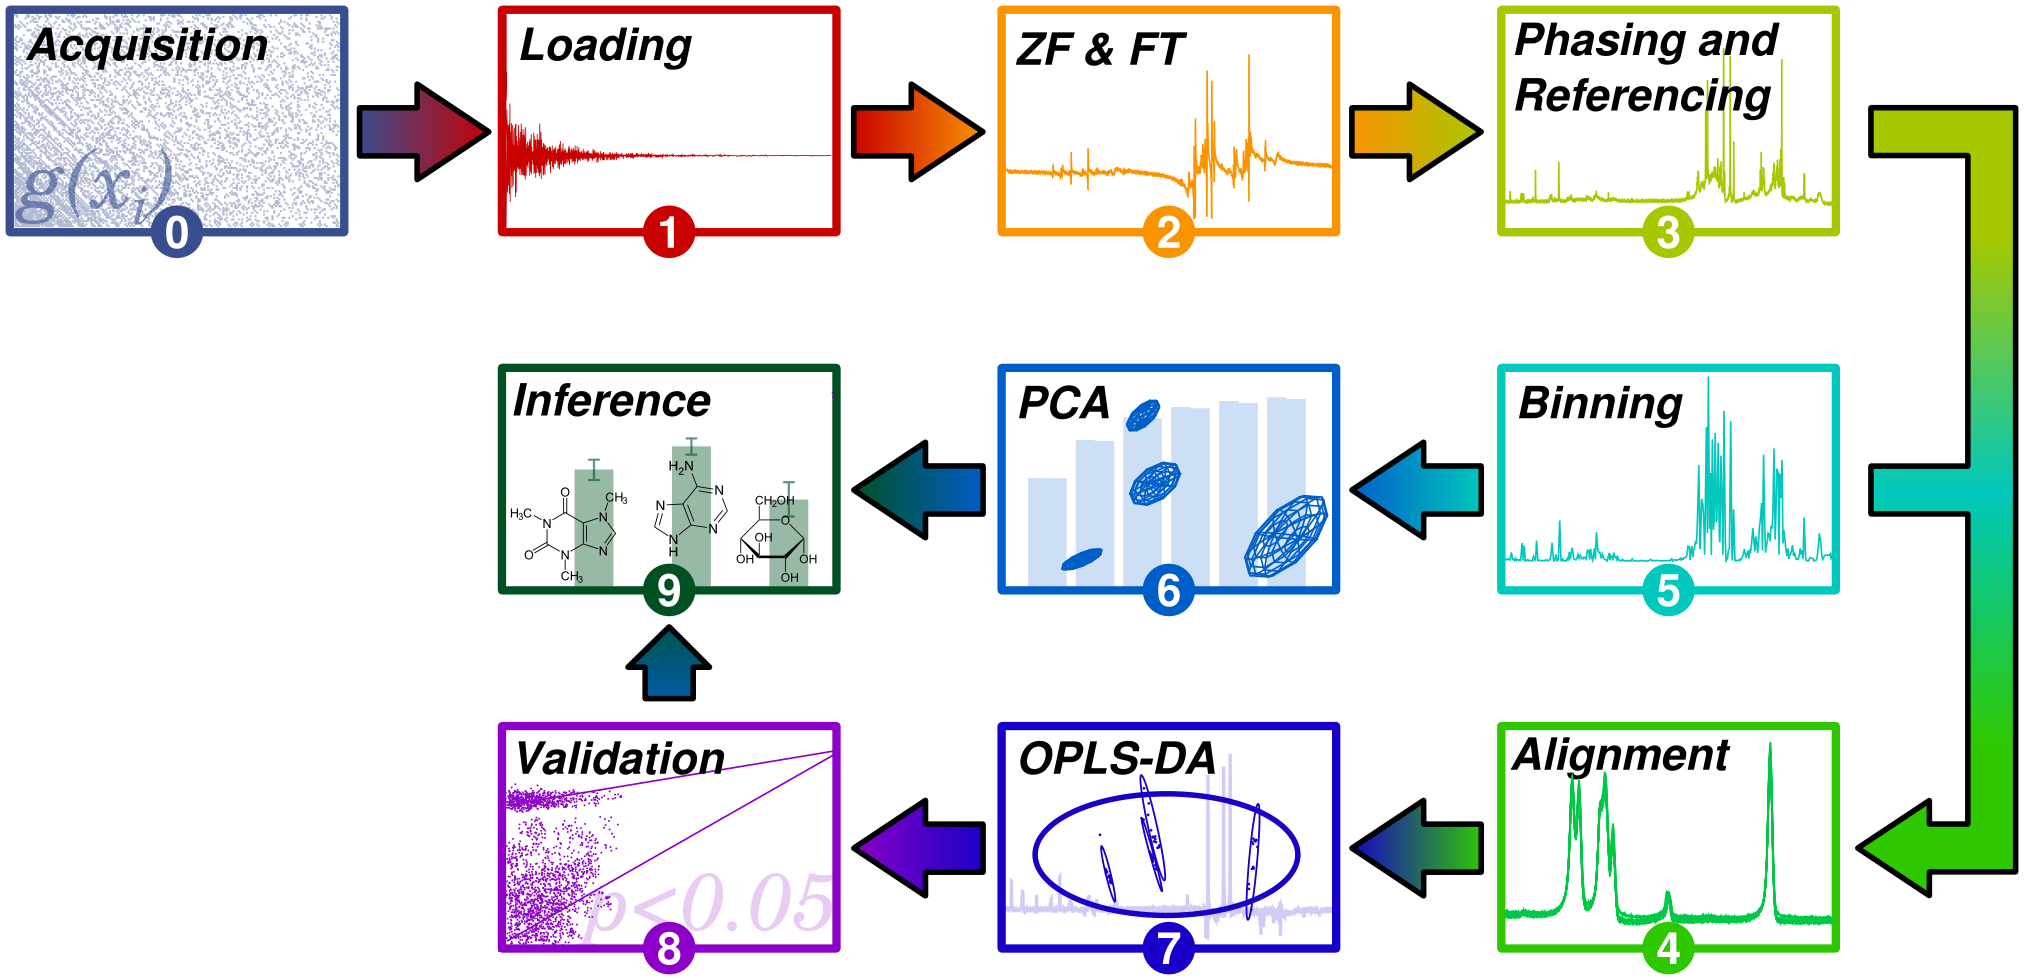
\includegraphics[width=5in]{figs/intro/01.png}
\end{center}
\caption
      [General Data Flow in Metabolomics.]{
  {\bf General Data Flow in Metabolomics.}
  \\
  Data in chemometric analyses of metabolism flows through this general graph,
  beginning at spectral data acquisition {\bf (0)}, through to loading and
  processing of instrumental data {\bf (1-3)}, further data treatment
  {\bf (4-5)}, mathematical modeling {\bf (6-7)} and model validation
  {\bf (8)}, and terminating on extraction of chemical information {\bf (9)}.
  In practice, this graph would be completely connected, and thus cyclic.
}
\end{figure}

\subsection{Acquisition}

\begin{doublespace}
Nuclear Magnetic Resonance (NMR) spectroscopy is a popular analytical platform
for chemometric analyses of protein structure and cellular metabolism, due to
its ability to simultaneously report atomic-level details of the chemical
environments and motional dynamics of \hnmr{}, \cnmr{} and \nnmr{} nuclei in
biomolecules \cite{abragam1961,levitt2008}. While the amount of
information contained within one-dimensional (1D) NMR spectra is high, it is
commonly held in a relatively narrow spectral width
(e.g. -2.0 -- 16 ppm for \hnmr{} spectra). As a result, 1D \hnmr{} NMR spectra
of complex metabolite mixtures or biomacromolecules suffer from severe signal
overlap that confounds analysis and interpretation.
\\\\
Ever since the introduction of two-dimensional NMR methods by Jeener and Ernst
\cite{ernst:chim1975,maudsley:cpl1977} and the popularization of
three-dimensional methods for studying proteins by Bax and colleagues
\cite{marion:jacs1989,kay:bioc1989}, NMR spectroscopists have been
leveraging \hcnmr{} and \hnnmr{} connectivities to spread biomolecular
information from 1D \hnmr{} spectra into two or more dimensions. While
multidimensional experiments alleviate signal overlap, they require
significantly more time to acquire than 1D spectra, as any $D$-dimensional
experiment is effectively a $(D-1)$-dimensional array of $2^{D-1}$
one-dimensional experiments. Time constraints imposed by throughput
requirements, sample stability and instrumental maintenance have historically
forced spectroscopists to harshly undersample their multidimensional datasets
in the time domain, resulting in frequency domain digital resolutions much
lower than the intrinsic linewidth of their samples
\cite{szyperski:pnas2002,rovnyak:jbnmr2004}.
\end{doublespace}

\begin{SCfigure}
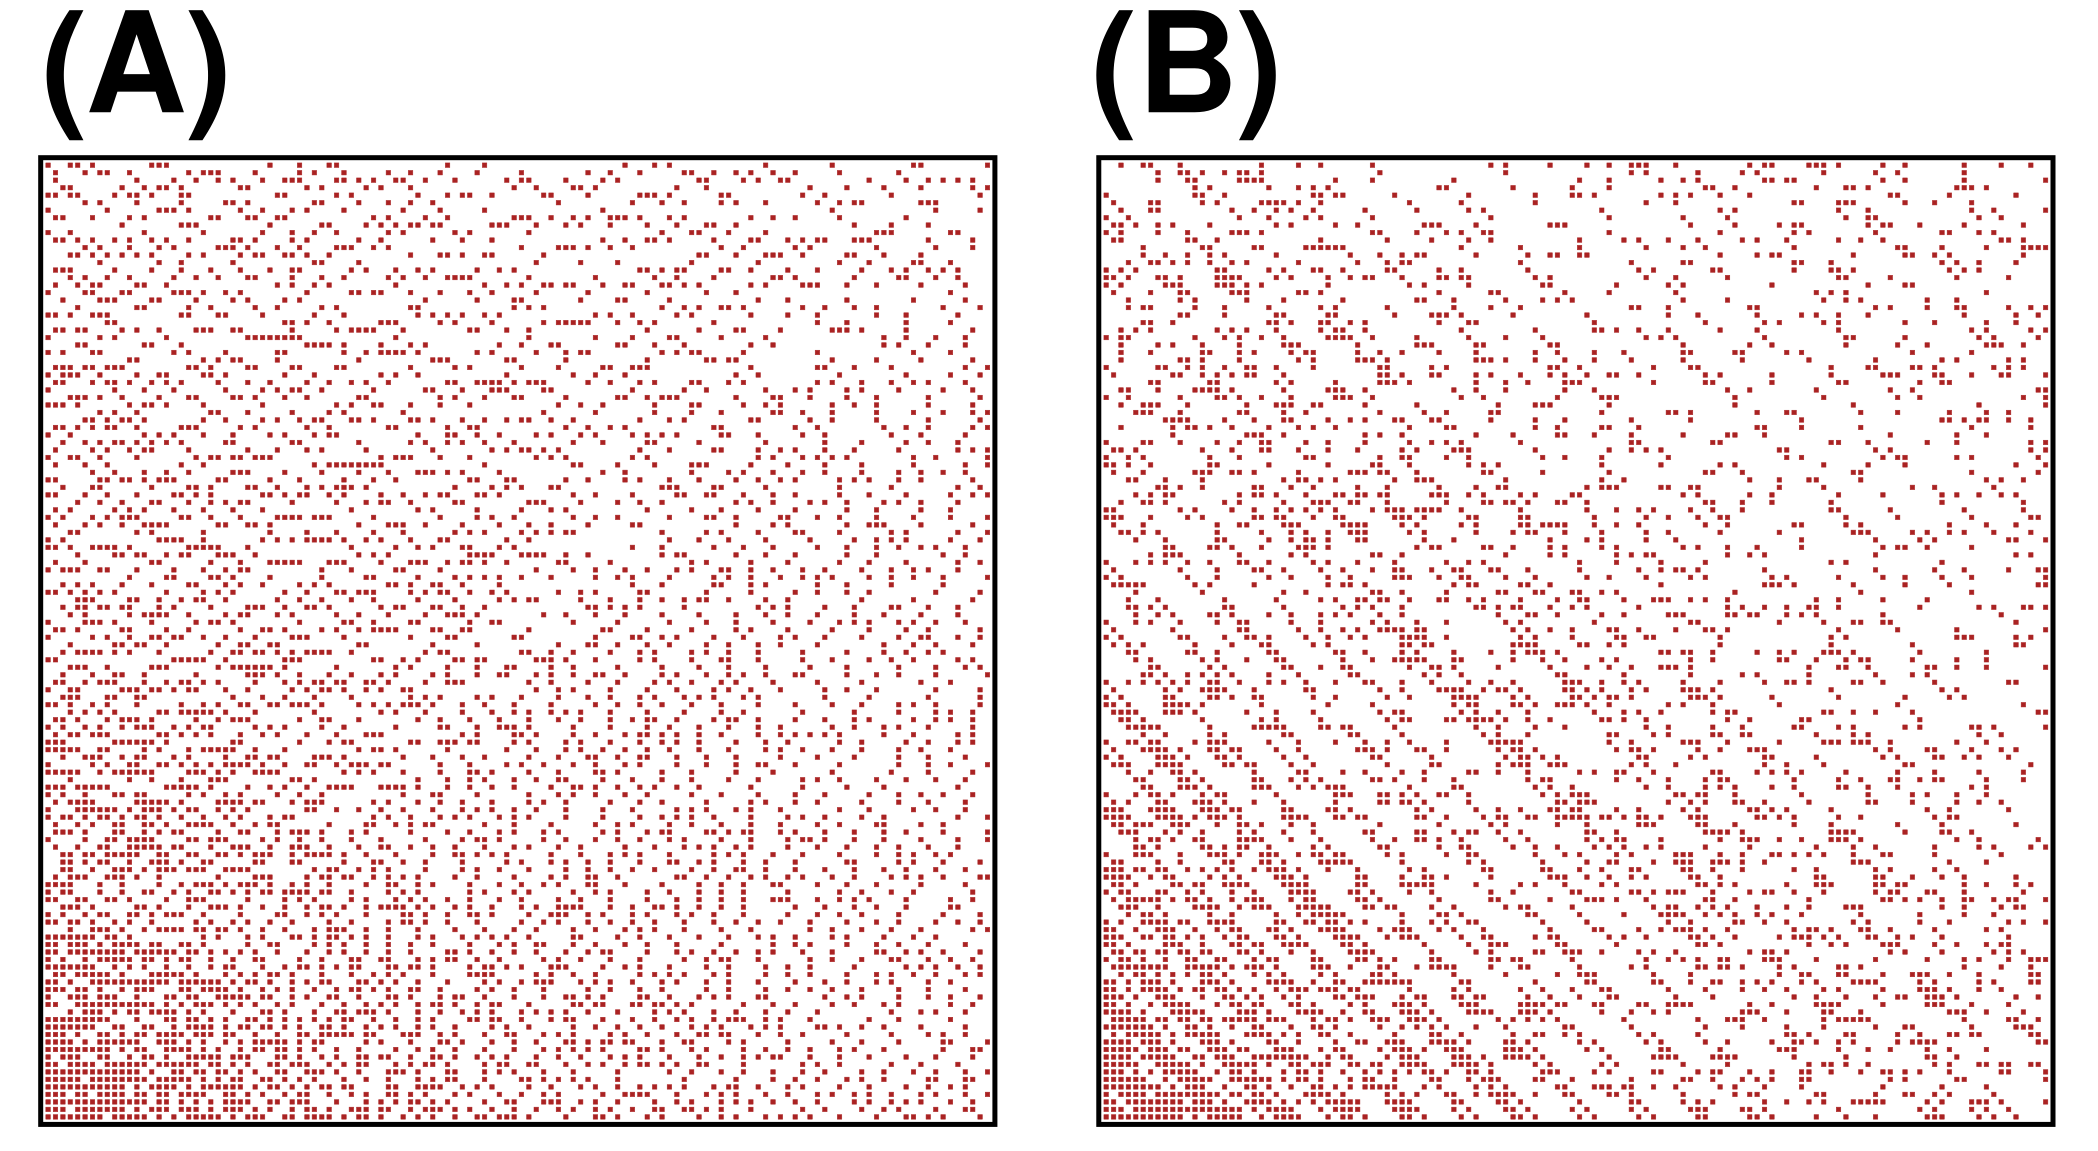
\includegraphics[width=3.5in]{figs/intro/02.png}
\caption
      [Example Nonuniform Sampling Schedules on a 2D Nyquist Grid.]{
  {\bf Example Nonuniform Sampling Schedules on a 2D Nyquist Grid.}
  \\
  Nonuniform sampling schedules produced by ({\bf A}) stochastic and
  ({\bf B}) deterministic subsampling of a two-dimensional Nyquist sampling
  grid. Comparisons of the performance of such schedules are made in
  Chapter 2.
}
\end{SCfigure}

\begin{doublespace}
In order to move from this ``sampling-limited'' regime of data acquisition,
the indirect dimensions of multidimensional NMR experiments may be nonuniformly
sparsely sampled (Figure 1.2), reducing the time required for data collection
while simultaneously enabling increased digital resolution
\cite{rovnyak:jmr2004}. When combined with non-Fourier reconstruction
algorithms such as Maximum Entropy, $L_1$-norm Minimization, and
Multidimensional Decomposition \cite{mobli:pnmrs2014}, this technique
of nonuniform sampling (NUS) is capable of producing high-quality,
high-resolution multidimensional spectra in a fraction of the time
required by traditional uniform sampling. However, the choice of which data
points to subsample from a uniform Nyquist grid is nontrivial and has typically
been made by random sampling methods
\cite{hoch:jmr2008,maciejewski:jmr2009}.
\end{doublespace}

\subsection{Processing and Treatment}

\begin{doublespace}
More often than not, effective chemometric modeling of raw experimental data
requires the data to be slightly modified from its original form. As an
example, two commonly utilized soft bilinear modeling algorithms, principal
component analysis (PCA, \cite{jolliffe2002}) and partial least squares
(PLS, \cite{wold1993}), analyze the eigenstructure of one or more data
matrices, and require subtraction of the sample mean and scaling by the sample
standard deviation in order to operate most effectively. When this modification
is instrumentation-specific, it is referred to as {\it processing}; otherwise,
it is considered a form of statistical {\it treatment}. The choice of which
processing and treatment methods to apply to a given dataset $\mathbf{D}$
varies, depending on how the data was collected, which model $f(\mathbf{D})$
is used, and what information is sought from the model by the analyst.
\\\\
Processing of NMR spectral datasets presents unique challenges to the analyst,
as each spectrum is collected in hypercomplex quadrature
\cite{schuyler:jmr2013} without absolute phase information. As a result,
NMR spectra must be phase-corrected to maximize the real spectral component
(cf. \hyperlink{chapter.3}{Chapter 3}). When multiple spectra are processed as
part of a statistical ensemble, any differences in phase {\it between} spectra
become a contributing factor to undesirable within-group variation that
inflates model errors. Thus, methods of phase-correcting multiple spectral
observations are required when those observations will become inputs into
multivariate modeling algorithms \cite{worley:cils2014}.
\\\\
Once instrument-specific processing has been performed on a dataset
$\mathbf{D}$, general statistical treatment operations may then be necessary,
depending on the model function $f(\mathbf{D})$ being utilized. One commonly
practiced method of preconditioning the eigenstructure of $\mathbf{D}$ for
PCA and PLS, known as binning or bucketing, involves partitioning $\mathbf{D}$
into smaller signal-containing spectral regions and integrating or vectorizing
those regions in order to achieve reduced data dimensionality. Multiple methods
of binning one-dimensional datasets have been developed, ranging from
na\"{\i}ve uniform subdivision algorithms
\cite{hedenstrom:cils2008,sousa:cils2013} to high-performance recursive
methods \cite{davis:cils2007,demeyer:anchem2008}. However, at the time
of this writing, no methods of intelligently (non-uniformly) binning
multidimensional datasets have been developed, essentially restricting bilinear
PCA and PLS modeling to using 1D \hnmr{} NMR spectral data in NMR chemometric
studies of metabolism.
\end{doublespace}

\begin{figure}[hb!]
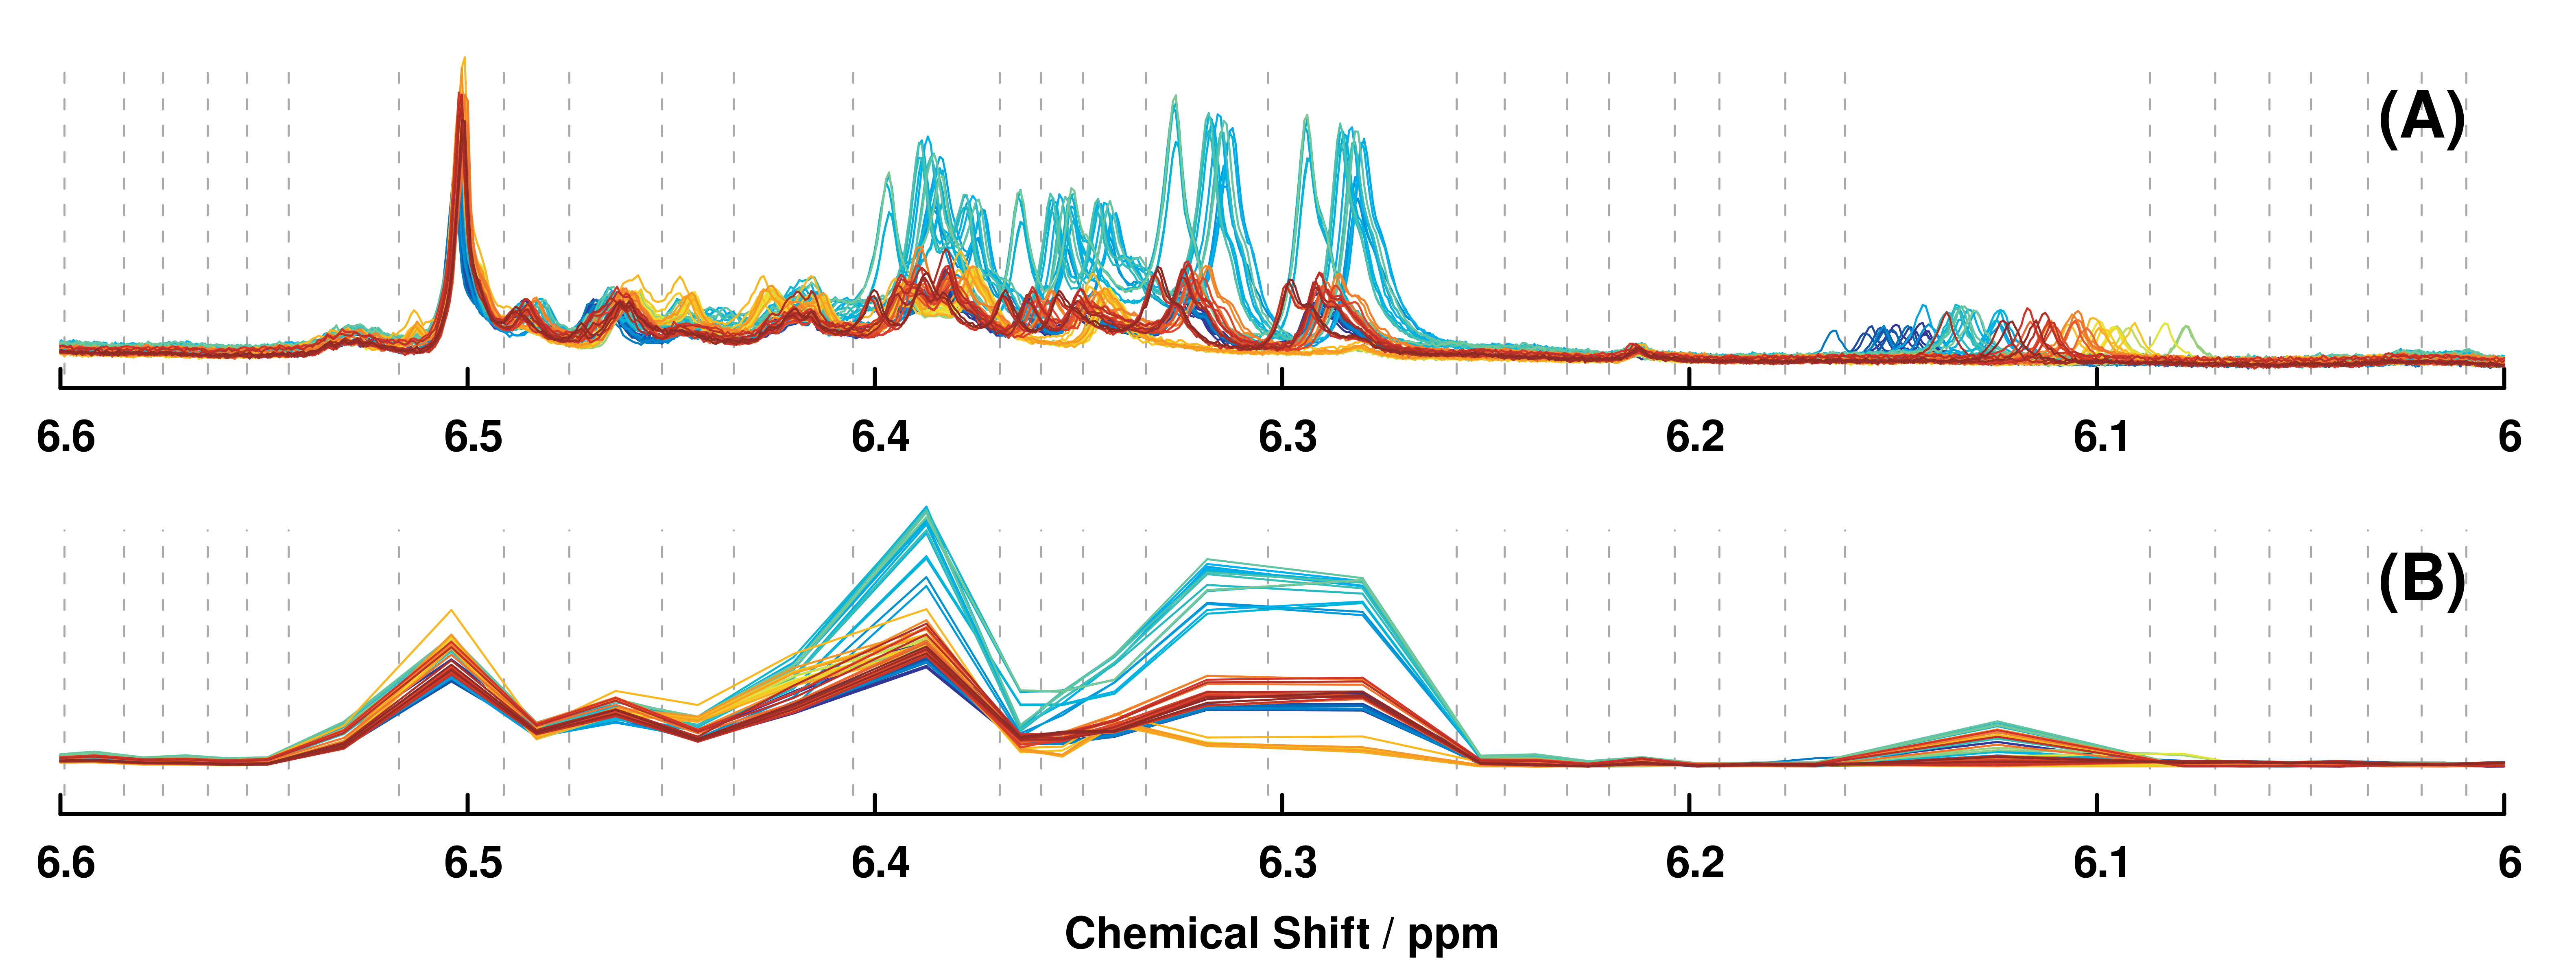
\includegraphics[width=6.5in]{figs/intro/03.png}
\caption
      [Example Binning Result from a 1D \hnmr{} NMR Dataset.]{
  {\bf Example Binning Result from a 1D \hnmr{} NMR Dataset.}
  \\
  Full-resolution ({\bf A}) and adaptively intelligently binned ({\bf B}) 1D
  \hnmr{} NMR spectra from a chemometric study of brewed coffee roasts.
  Spectral color indicates the observation index, and dashed lines indicate bin
  boundaries. Further discussion of binning may be found in Chapters 3 and 6.
}
\end{figure}

\subsection{Modeling and Validation}

\begin{doublespace}
Once a dataset $\mathbf{D}$ has been suitably processed and treated, a model
$f(\mathbf{D})$ may be trained on its contents. Within chemometrics, principal
component analysis (PCA) is undoubtedly the most routinely used modeling
algorithm for describing relationships between multivariate spectral
observations \cite{bro:anmeth2014}, because it provides an unbiased,
simplified picture of the data in a low-dimensional ``scores'' space. The
scores obtained from PCA models of spectral data are useful for determining
statistical distances between experimental groups
\cite{demaesschalck:cils2000,worley:abio2013}, which are effective predictors
of the reliability of any regression models that may be trained on the same
data.
\\\\
Another multivariate algorithm of equal popularity to PCA in chemometrics is
partial least squares (PLS), which is used for solving regression and class
discrimination problems on multivariate data \cite{wold1993}. While PLS
provides a similar low-dimensional scores-space view of spectral observations,
its true power in chemometrics lies in its ability to report ``loadings'',
which are spectral contributions that predict a set of chemical properties.
\\\\
The combination of PCA and PLS as a methodology for studying complex spectral
datasets has proven highly useful in chemometrics, most notably so in the
field of metabolomics \cite{lindon:cmr2000}. However, analysts must take care
when using models produced by these methods, as they have not been determined
using standard (over-determined) least-squares methods and may over-fit a
dataset at the expense of generality, which is required for broad inference
\cite{westerhuis:metab2008}. Rigorous application of cross-validation methods,
including internal and external cross-validation
\cite{xu:cils2001,eshghi:cils2014}, response permutation testing
\cite{golland:learn2005} and CV-ANOVA \cite{eriksson:jchemo2008}, is required
in order to ensure that trained multivariate models are reliable and
generalizable to later measurements.
\end{doublespace}

\subsection{Inference}

\begin{doublespace}
Once multivariate models have been trained and validated on a given dataset,
they may finally be utilized for the extraction of chemical information from
that dataset. Often, this process of inference revolves around the analysis of
separations between one or more experimental groups in PCA or PLS scores space.
Because scores-space separations are often used as justification for further
costly experimentation, it is important to quantitatively measure these
separations using proper statistical tools \cite{worley:abio2013}.
\end{doublespace}

\section{Summary of Work}

\begin{doublespace}
By and large, this dissertation follows the logical flow of a data analyst
in the field of NMR metabolomics, working from methods in compressive data
acquisition, through a description of multivariate analysis techniques, to
processing, treatment and validation of multivariate modeling results, and
ending with a solution to a bioinformatics data handling problem: the
correlation between high-resolution protein structure and backbone chemical
shifts.
\\\\
\hyperlink{chapter.2}{Chapter 2} begins by introducing a gap-based nonuniform
sampling framework that provides several attractive advantages over traditional
probability density-based nonuniform sampling methods. While most methods of
generating nonuniform sampling schedules rely on randomly sampling from a
specified weighting function that is defined over a Nyquist grid, this new
method of gap sampling builds up schedules based on the value of a `gap
equation' that specifies the spacing between sampled Nyquist grid points. The
gap sampling framework is first defined, and comparisons in performance are
made between specific forms of gap sampling and the stochastic Poisson-gap
sampling method from Hyberts and Wagner \cite{hyberts:jacs2010}.
\\\\
A comprehensive description of the required data handling tasks -- steps
{\bf (1-9)} in Figure 1.1 -- in metabolic fingerprinting and untargeted
metabolic profiling studies is provided within
\hyperlink{chapter.3}{Chapter 3}. Additional practical guidelines on the
relationship between class separations in PCA scores space and reliability
of OPLS-DA models on the same data are also presented.
\\\\
\hyperlink{chapter.4}{Chapter 4} introduces the MVAPACK toolbox for
chemometrics as a complete solution to the data handling problem in NMR-
and MS-based metabolomics studies. Beginning with a set of raw free induction
decays from an NMR spectrometer, analysts may now rapidly and easily generate
validated multivariate models using rigorously tested and peer-reviewed
routines in MVAPACK. As a result, both the turnaround time between data
collection and interpretation and the likelihood of analyst error are
dramatically reduced when using MVAPACK. The architecture and design rationale
of the MVAPACK toolbox are discussed in this chapter.
\\\\
\hyperlink{chapter.5}{Chapter 5} and \hyperlink{chapter.6}{Chapter 6} focus on
two novel methods of data processing (Phase-Scatter Correction) and treatment
(Generalized Adaptive Intelligent Binning) that were developed within the
MVAPACK toolbox specifically for efficient management of NMR spectral data.
\hyperlink{chapter.7}{Chapter 7} describes a small set of portable utilities
that generate statistically sound dendrograms of scores-space class
relationships using both bootstrap-based and parametric methods.
\\\\
\hyperlink{chapter.8}{Chapter 8} outlines the generation of a set of
bioinformatic tools to analyze the relationship between the geometry of
interacting pairs of carbonyls in protein backbones and their \cnmr{} chemical
shift values \cite{worley:pone2012}. These tools, combined with quantum
chemical computations, provide strong evidence for the nonexistence of
\npistar{} interactions between these carbonyl groups in native protein
structures.
\\\\
Finally, \hyperlink{chapter.9}{Chapter 9} summarizes the solutions provided
herein to a set of chemometrics and bioinformatics data handling problems and
discusses challenges and avenues of effort that will be required to solve
future problems of the same kind.
\end{doublespace}

\bibliographystyle{abbrv}
\bibliography{bworley}



\chapter{Multidimensional Nonuniform Gap Sampling}

\begin{quote}
{\it
  Anyone who considers arithmetical methods of producing random digits is,
  of course, in a state of sin.}
\\\\
 -- John von Neumann
\end{quote}

\section{Introduction}

FIXME \cite{mobli:jmr2015}.

\bibliographystyle{abbrv}
\bibliography{bworley}



\chapter{Multivariate Analysis in Metabolomics}

\begin{quote}
{\it Essentially, all models are wrong, but some are useful.}
\\\\
 -- George E. P. Box
\end{quote}

\section{Introduction}

\begin{doublespace}
The applications of chemometrics are as broad as the field of chemistry itself,
but one particularly challenging subdiscipline of bioanalytical chemistry --
known as ``metabolomics'' -- has recently renewed interest in the use of
chemometrics \cite{worley:cmb2013}. Indeed, the chemical complexity of
systems studied by metabolomics {\it necessitates} the use of chemometric
techniques: if metabolomics were a nail, chemometrics would surely be a hammer.
\\\\
Metabolomics is defined \cite{lindon:cmr2000} as ``the quantitative
measurement of the multiparametric metabolic response of living systems to
pathophysiological stimuli or genetic modification.'' Such a definition implies
that metabolomics studies offer the finest-grained detail available in the
nascent field of systems biology: a molecular-level convolution of all upstream
genomic, transcriptomic and proteomic responses of an organism to a given
stimulus or change
\cite{kell:opin2004,trethewey:opin2001,weckwerth:arpb2003}. Metabolites
are the end product of all cellular processes, and their in vivo
concentrations are a direct result of enzymatic activity. While a change in the
expression level of a protein or its coding gene may not necessarily correlate
directly with the activity of that protein, alterations in metabolite
concentrations {\it are} the consequence of altered activity
\cite{terkuile:febs2001}. Thus, metabolites are more proximal to a
phenotype or disease state than either genetic or proteomic information. The
richness of phenotypic information offered by metabolomics has been leveraged
to identify disease biomarkers
\cite{gebregiworgis:cchts2012,vinayavekhin:acscb2010}, to aid in
the drug discovery process \cite{powers:mrc2009,wilcoxen:eodd2010}, and to
study plants \cite{hall:pcell2002}, bacteria
\cite{zhang:jiomic2013,tang:cgen2011}, nutrition
\cite{mcniven:jnb2011}, and the environment
\cite{bundy:metab2009}, among numerous other applications
\cite{baker:nmeth2011}.
\\\\
The rich information promised by metabolomics does not come without a price,
and metabolomics experiments are plagued with difficulty. The number of
small-molecule metabolites in a biofluid, cell lysate, tissue or organ differs
wildly depending on the organism studied, ranging from several hundered to
hundreds of thousands \cite{dunn:trac2005}. While databases of commonly
encountered metabolites have been compiled
\cite{wishart:nar2007,cui:nbiot2008,kind:anchem2009}, they are by no
means complete. Therefore, it is common to encounter unknown signals during
data analysis, complicating the interpretation of metabolic changes between
experimental groups. Metabolite identification is further complicated by a
lack of NMR or mass spectral reference information for known metabolites.
Finally, the diversity of chemical and physical properties of metabolites
makes true simultaneous quantitation of all metabolites present in a system
unattainable with current instrumental capabilities
\cite{lindon:cmr2000,dunn:trac2005,dettmer:msr2007}. As an illustration,
due to the limited molecular mass distribution of the metabolome, comprehensive
metabolomic analyses by mass spectrometry generally require the prefixing of
one or more chromatographic separations prior to analyte ionization
\cite{kell:opin2004,viswanadhan:acsccc2011}.
\\\\
The extraction of information from data in metabolomics experiments is further
complicated by the inherent variability present within each sample. Every
single cell, tissue, organ or organism is fundamentally unique
\cite{rubakhin:nmeth2011}, despite any features (disease state, drug
treatment, {\it etc.}) it may have in common with others of its kind. Thus,
the differentiation between two experimental groups in a metabolomics
experiment requires the identification of relatively few defining or
discriminating chemical features against a large, complex background of
metabolites \cite{wishart:nar2007}. Ideally, these few chemical features
may be identified as a unique set of metabolites that are directly related to
the defining biochemical states of each experimental group. Unfortunately, all
biological systems are easily perturbed by experimental or environmental
factors, including age, gender, diet, cell growth phase, nutrient availability,
pH and temperature \cite{tyagi:ijpsrr2010,zhang:jiomic2013}. Variations in
sample handling procedures, including cell lysis, metabolic quenching,
metabolite extraction and sample storage can also introduce further variability
into the measured data. Finally, variations in signal position, intensity and
shape may manifest from instrumental instabilities on a per-sample basis.
Each of these numerous sources of sample variability increases the magnitude of
$\mathbf{E}$ in any chemometric model that may be applied to the data
(cf. \hyperlink{section.1.1}{Section 1.1}), which decreases the statistical
validity of $f(\mathbf{D})$. Therefore, the design of experiments and analysis
of data in metabolomics requires robust methodologies in order to expose
underlying chemical trends from highly complex systems in the form of
statistically valid mathematical models. This chapter describes the theory
and best practices of chemometric analyses of data produced by metabolomics
experiments, with a focus on 1D \hnmr{} and 2D \hcnmr{} NMR datasets.
\end{doublespace}

\begin{figure}[ht!]
\begin{center}
  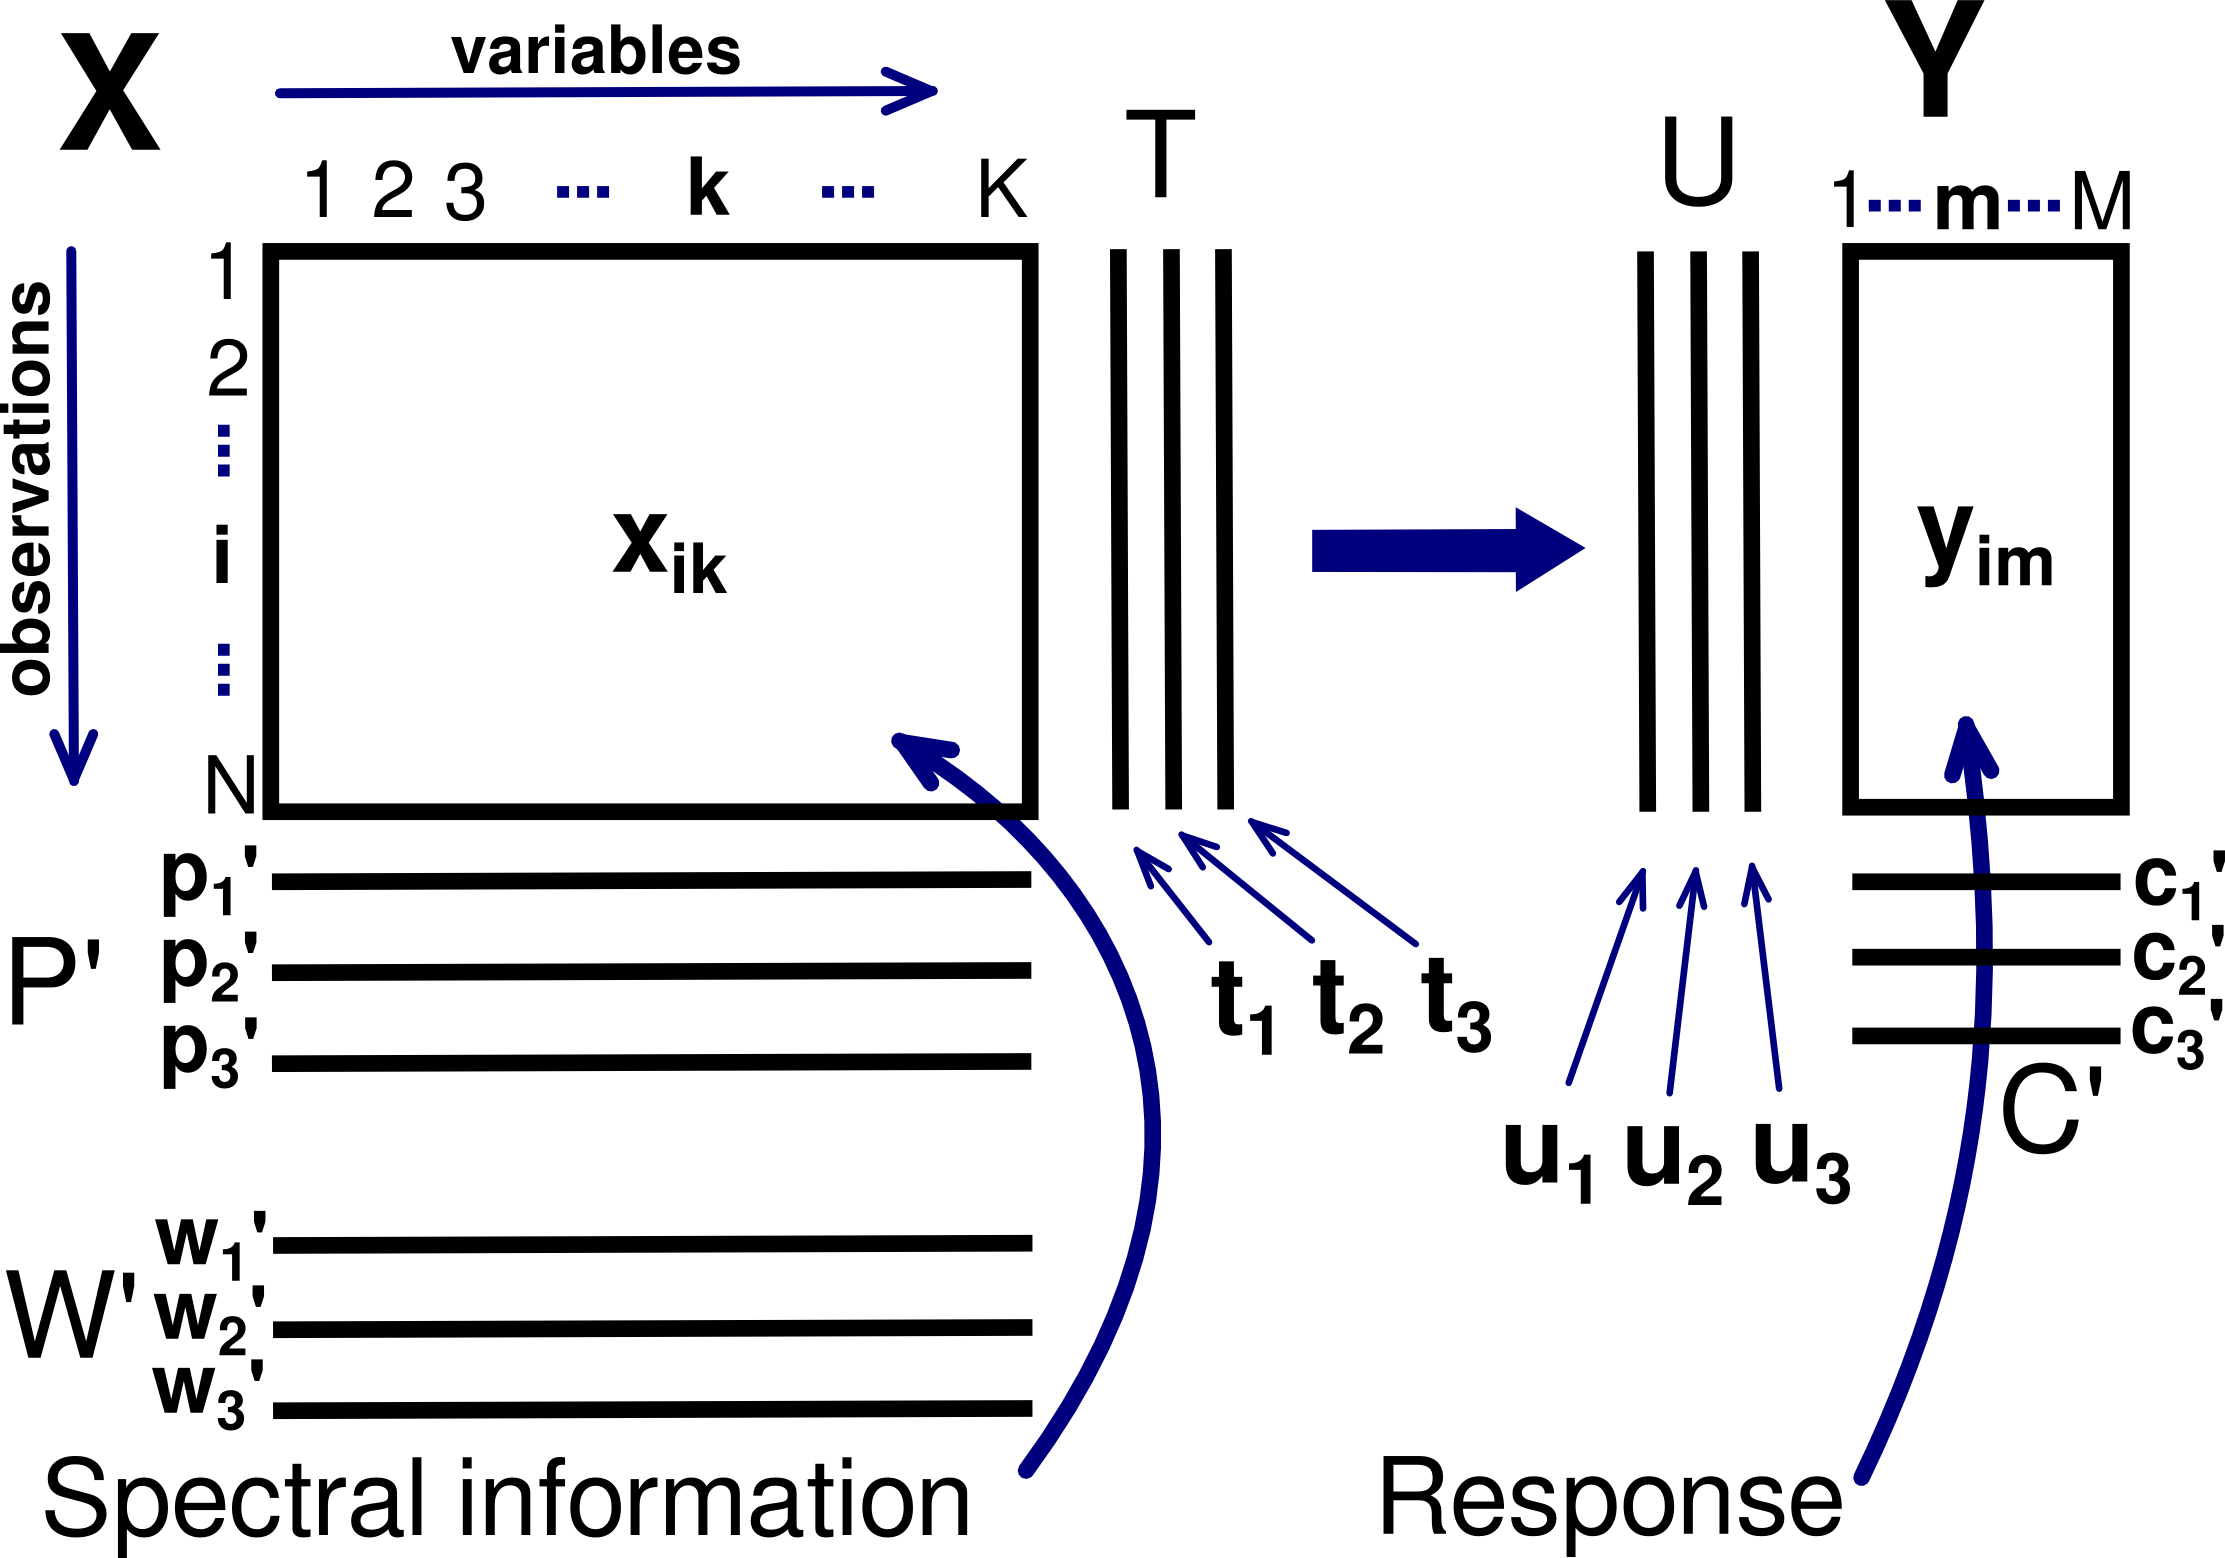
\includegraphics[width=4in]{figs/mva/01.png}
\end{center}
\caption
      [Canonical Example of a Bilinear Modeling Problem.]{
  {\bf Canonical Example of a Bilinear Modeling Problem.}
  \\
  Illustration of a data matrix $\mathbf{X}$ and a response matrix
  $\mathbf{Y}$, as they are typically used in partial least squares
  modeling problems. In metabolomics applications, the data matrix will
  contain a set of $N$ spectra, each having $K$ variables. For supervised
  modeling problems, each observation in the data matrix is paired with a
  corresponding row in the response matrix that holds either continuously
  varying outputs or binary class memberships. The data are then decomposed
  into a small number of score vectors ($\mathbf{t}$) and loading vectors
  ($\mathbf{p}$), with corresponding weight vectors ($\mathbf{w}$) used
  to transform the observations in $\mathbf{X}$ into scores-space. The
  responses in $\mathbf{Y}$ are similarly decomposed into scores
  ($\mathbf{u}$) and loadings ($\mathbf{c}$). Tick marks denote
  transposition.
}
\end{figure}

\section{Multivariate Datasets}

\begin{doublespace}
In the majority of cases, multivariate datasets used in metabolomics take the
form of second-order tensors in $\mathbb{R}^{N \times K}$. More simply, these
datasets are real matrices having $N$ rows and $K$ columns. By convention,
the data are arranged as $N$ observation row vectors of length $K$, where $K$
is referred to as the dimensionality of the dataset (Figure 3.1). Typical
examples of 1D datasets include sets of \hnmr{} or \cnmr{} NMR spectra
\cite{beckonert:nprot2007,koh:colon2009}, direct-injection mass spectra
(DI-MS, \cite{castrillo:phch2003,southam:anchem2007,zhou:asms2010}), infrared
(IR) and Raman spectra \cite{ellis:analyst2006,cherney:anchem2007}, or
capillary electrophoretograms (CE, \cite{ramautar:trac2006}). This remarkable
diversity of instrumental platforms used in metabolomics is traceable to the
ability of bilinear factorizations such as principal component analysis
(PCA, \cite{jolliffe2002}) and partial least squares (PLS, \cite{wold1993}) to
directly accept these second-order tensors for modeling (vide infra).
\\\\
The dimensionality of a multivariate dataset may be increased by adding another
``mode'', resulting in a third-order (or higher) tensor
($\mathbf{X} \in \mathbb{R}^{N \times K_1 \times K_2}$, Figure 3.2). In such
cases, the total dimensionality of the dataset is now the product of the
dimensionalities along each mode of the data tensor (e.g. $K_1 \times K_2$).
Third-order tensors are the natural data structures for sets of two-dimensional
observations, including \hhnmr{}, \hcnmr{} and \hnnmr{} NMR spectra, hyphenated
chromatography-mass spectra (LC-MS, GC-MS), hyphenated electrophoresis-mass
spectra (CE-MS), and hyphenated ion-mobility mass spectra (IM-MS). While
third-order data tensors may hold substantially more chemical information than
their second-order counterparts, they are not directly compatible with bilinear
factorization methods, and they require specialized processing,
treatment and modeling algorithms \cite{lu:ieee2009,lu:pr2011}. As an example,
tensors may be vectorized into matrices \cite{hedenstrom:cils2008} that are
suited for PCA and PLS, but at the cost of lost structural information. Methods
such as uncorrelated multilinear PCA (UMPCA, \cite{lu:ieee2009}), on the other
hand, provide a means of directly decomposing tensors into low-dimensional
spaces while maintaining structural information.
\end{doublespace}

\begin{SCfigure}
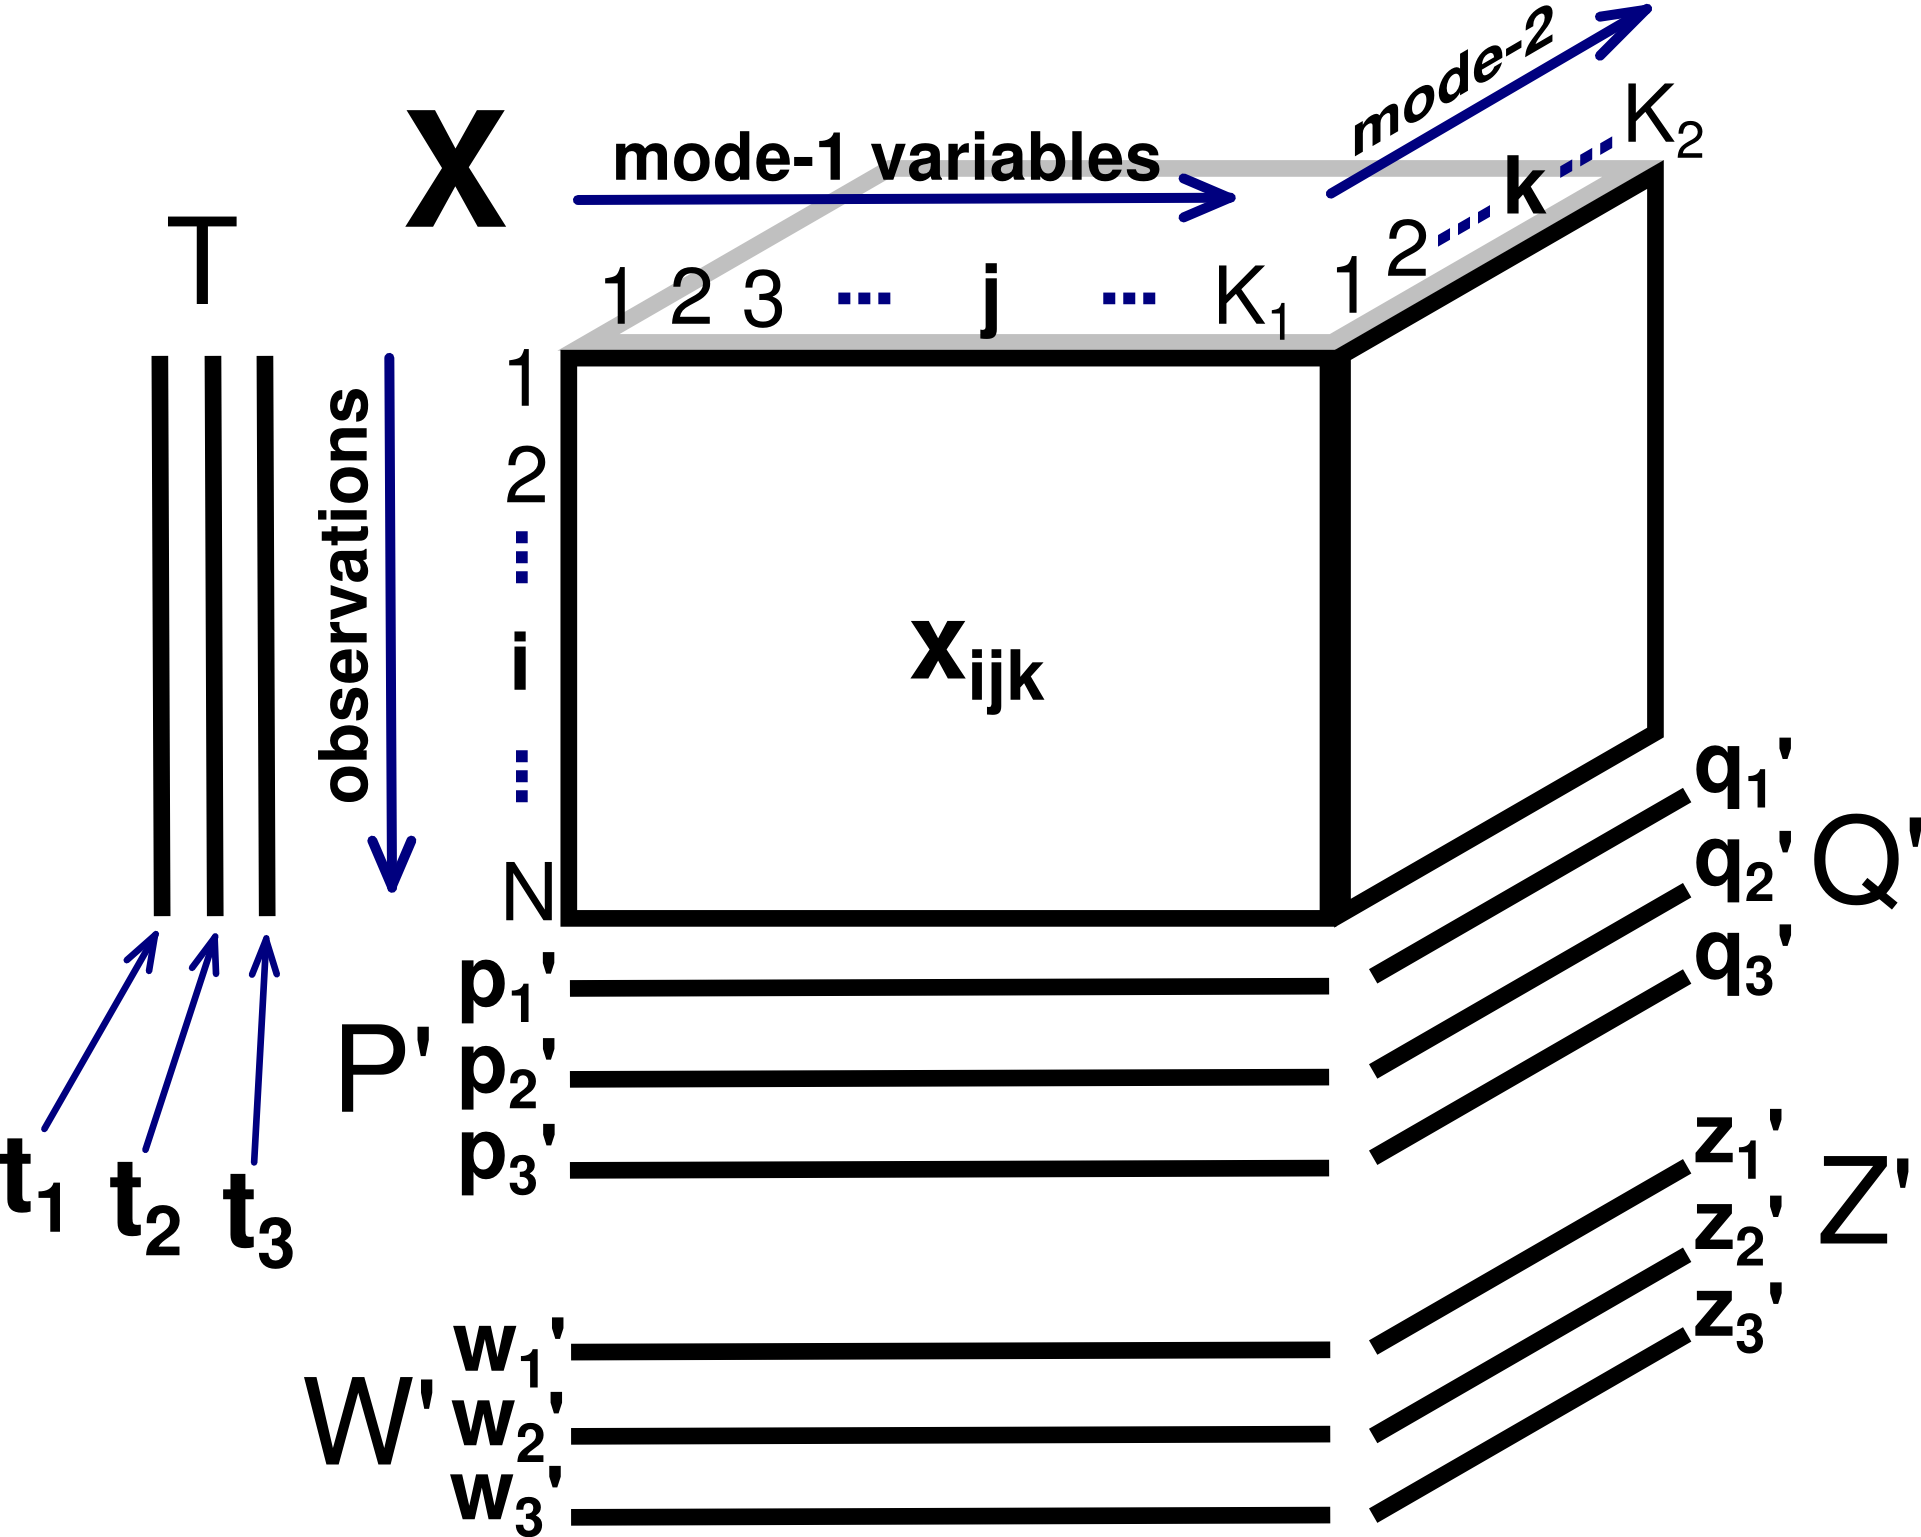
\includegraphics[width=3.5in]{figs/mva/02.png}
\caption
      [Canonical Example of an Unsupervised Trilinear Modeling Problem.]{
  {\bf Canonical Example of an Unsupervised Trilinear Modeling Problem.}
  \\
  Illustration of a third-order data tensor $\mathbf{X}$ as may be found in
  multilinear factorization problems. Such data tensors will contain a set
  of $N$ spectra, each having $K_1$ variables along their first mode and
  $K_2$ variables along their second. The data tensor is then decomposed
  into a small number of score vectors ($\mathbf{t}$) and loading vectors
  ($\mathbf{p}$, $\mathbf{q}$), with corresponding weight vectors
  ($\mathbf{w}$, $\mathbf{z}$) used to transform the observations in
  $\mathbf{X}$ into scores-space. Tick marks denote transposition.
}
\end{SCfigure}

\begin{figure}[hb!]
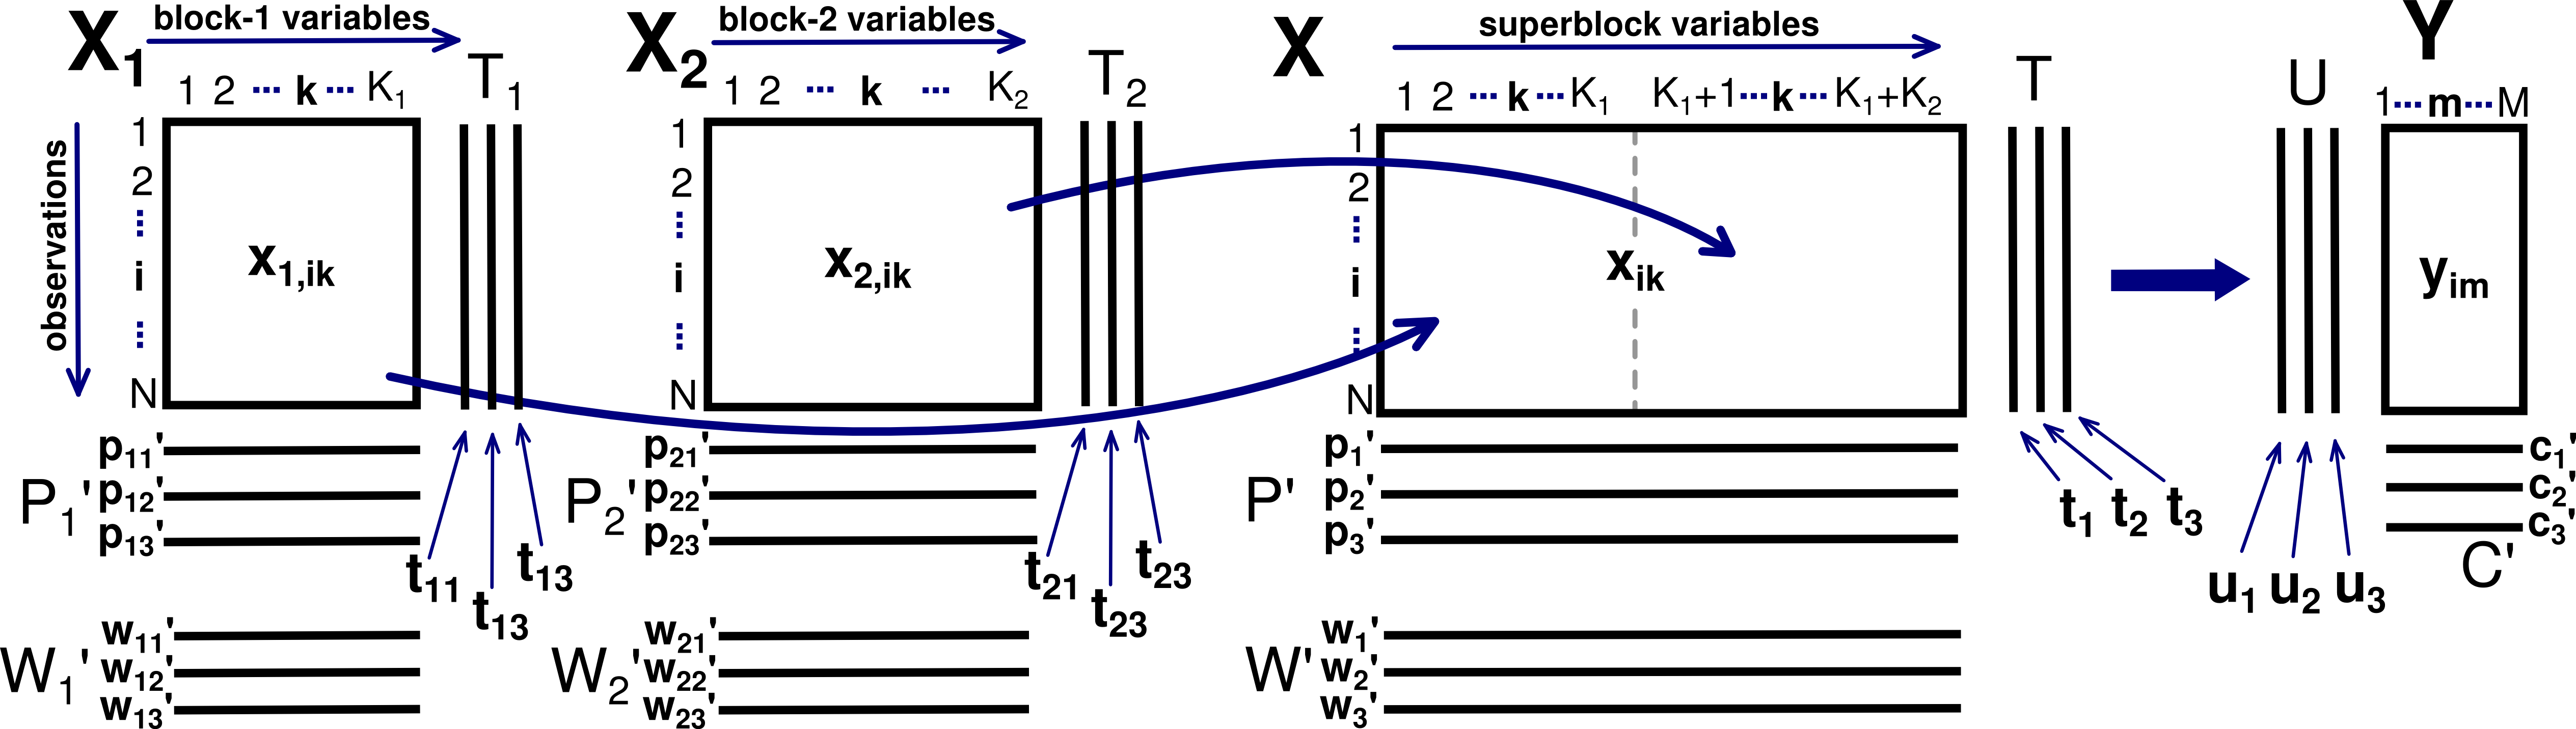
\includegraphics[width=6.5in]{figs/mva/03.png}
\caption
      [Canonical Example of a Multiblock Bilinear Modeling Problem.]{
  {\bf Canonical Example of a Multiblock Bilinear Modeling Problem.}
  \\
  Illustration of a pair of data matrices $\mathbf{X_1}$ and $\mathbf{X_2}$,
  their observation-wise concatenation $\mathbf{X}$, and a response matrix
  $\mathbf{Y}$, as they are typically used in multiblock partial least squares
  modeling problems. In metabolomics applications, each data matrix
  $\mathbf{X_b}$ in the set of $B$ matrices will contain a set of $N$ spectra,
  each having $K_b$ variables. The data are then decomposed into a small number
  of superblock score vectors ($\mathbf{t}$) and superblock loading vectors
  ($\mathbf{p}$), with corresponding superblock weight vectors ($\mathbf{w}$).
  Each individual data matrix is also decomposed into a set of block scores
  ($\mathbf{t_b}$), block loadings ($\mathbf{p_b}$) and block weights
  ($\mathbf{w_b}$). Tick marks denote transposition.
}
\end{figure}

\begin{doublespace}
Another mechanism of increasing the information content of datasets entering
into multivariate chemometric models is to collect spectral observations on
two or more complementary instrumental platforms for each sample. In such a
``multiblock'' modeling approach, each data block $\mathbf{X_b}$ contains $N$
$K_b$-variate observations \cite{westerhuis:jchemo1998,smilde:jchemo2003}.
Bilinear methods such as consensus PCA (CPCA), hierarchical PCA and PLS, and
multiblock PLS may then be used to provide information about data variation
that is correlated between data blocks. Recent examples of multiblock modeling
in metabolomics include fusions of near-IR and mid-IR spectra
\cite{bras:cils2005}, \hnmr{} NMR and direct injection electrospray mass
spectra (DI-ESI-MS, \cite{marshall:metab2015}), and observations from multiple
sensors in process control applications \cite{ferreira:jchemo2010}.
\end{doublespace}

\section{Spectral Processing}

\begin{doublespace}
Following the acquisition of experimental data, instrumentation-specific
processing must be applied to transform the data into a suitable set of
real matrices for bilinear modeling, or tensors for multilinear modeling.
Because the majority of data presented herein originated from an NMR
spectrometer, and because NMR spectra present unique challenges to the
analyst during data handling, the following discussions will center around
processing of 1D and 2D NMR datasets.
\end{doublespace}

\subsection{NMR Signals}

\begin{doublespace}
Modern NMR spectrometers effectively acquire a rotating-frame free induction
decay (FID) through the use of quadrature phase detection of the incoming
signal \cite{levitt2008}. This detection method imparts relative phase
information to the time-domain decays by creating an ``in-phase'' signal
component $i(t)$ and a ``quadrature'' component $q(t)$ phased ninety degrees
from $i(t)$. Indirect dimensions of multidimensional NMR experiments are also
collected in quadrature through interleaved acquisition of one-dimensional
decays that have been cosine- and sine-modulated by the indirect-dimension
signals \cite{states:jmr1982}. As a result, each data point in a
$D$-dimensional NMR signal collected in complete quadrature exists in a
hypercomplex space $\mathbb{H}_D$ \cite{schuyler:jmr2013}, which is defined by
a real basis element and $D$ complex basis elements:

\begin{equation}
\Phi_D \equiv \{ 1 \cdot u_1 \cdots u_D \}
\end{equation}

where multiplication by any complex element $u_d$ results in a ninety degree
phase shift in dimension $d$, and the basis elements combine commutatively
under multiplication, as follows:
\begin{align}
u_i u_j =& u_j u_i \\
u_i^2 =& -1
\end{align}

The basis elements in $\Phi_D$ are a generating set for the complete set of
components of the hypercomplex space $\mathbb{H}_D$. For example, in three
dimensions:

\begin{equation}
\Phi_3 = \{ 1, u_1, u_2, u_1 u_2, u_3, u_1 u_3, u_2 u_3, u_1 u_2 u_3 \}
\end{equation}

A scalar in $\mathbb{H}_D$ is then expressed as a linear combination of this
component set. For the three-dimensional example:

\begin{equation}
x = a + b u_1 + c u_2 + d u_1 u_2
  + e u_3 + f u_1 u_3 + g u_2 u_3 + h u_1 u_2 u_3
\end{equation}

or, more generally and succinctly:

\begin{equation}
x = \sum_{\phi \in \Phi_D} x \{ \phi \} \cdot \phi
\end{equation}

where $x\{\phi\}$ denotes the real coefficient of $x$ that scales the basis
component $\phi$ in $x$. For the above three-dimensional example, the
expression $x\{u_1 u_3\}$ would evaluate to $f$. Finally, the expression of
hypercomplex tensors is formally accomplished by defining each coefficient
as a real tensor of appropriate size, like so:

\begin{equation}
x \{ \phi \} \in \mathbb{R}^{k_1 \cdots k_K} \quad \forall \phi \in \Phi_D
\end{equation}

where $K$ is the number of modes of the tensor. The above equation may be
compactly written as $\mathbb{H}_D^{k_1 \cdots k_K}$. Any scalar
in $\mathbb{H}_D$ -- and therefore any data point in a $D$-dimensional
quadrature-complete NMR dataset -- shall require $2^D$ real coefficients
in order to be completely determined. While the hypercomplex
algebras $\mathbb{H}_0$ and $\mathbb{H}_1$ are isomorphic to the real 
($\mathbb{R}$) and complex ($\mathbb{C}$) numbers, respectively, $\mathbb{H}_2$
and $\mathbb{H}_3$ are {\it not} isomorphic to the quaternions and octonions,
as the latter are noncommutative under multiplication. This hypercomplex
algebra, introduced for partial-component nonuniform subsampling by Schuyler
et al. \cite{schuyler:jmr2013}, provides an elegant formalism for expressing
and handling NMR data.
\\\\
Mathematically, 1D NMR free induction decays are described by the following
commonly used parametric signal model:

\begin{equation}
f(t) = \sum_{m=1}^M \alpha_m \exp\left\{
  u_1 (\omega_m t + \theta_m) - \rho_m t
  \right\}
\end{equation}

where $\alpha_m$, $\omega_m$, $\theta_m$ and $\rho_m$ represent the amplitude,
frequency, phase error and decay rate of the $m$-th damped complex exponential
in the model $f(t)$. Using the above formalism for hypercomplex tensors, this
signal model is trivially extended to any number of dimensions by multiplying
in a modulation term for each dimension:

\begin{equation}
f(\mathbf{t}) = \sum_{m=1}^M \alpha_m \prod_{d=1}^D \exp\left\{
  u_d (\omega_{m,d} t_d + \theta_{m,d}) - \rho_{m,d} t_d
  \right\}
\end{equation}

For example, a 2D FID may be modeled as follows:

\begin{equation}
f(t_1, t_2) = \sum_{m=1}^M \alpha_m \exp\left\{
  u_1 (\omega_{m,1} t_1 + \theta_{m,1}) +
  u_2 (\omega_{m,1} t_2 + \theta_{m,2}) -
  \rho_{m,1} t_1 - \rho_{m,2} t_2
  \right\}
\end{equation}

In short, NMR free induction decays may be treated as sums of damped
hypercomplex exponentials. While it is possible to directly parameterize
$f(\mathbf{t})$ using either maximum likelihood estimation
\cite{chylla:jbnmr1995,chylla:jbnmr1998,chylla:anchem2011} or Bayesian
model selection and estimation
\cite{bretthorst:jmr1990a,
      bretthorst:jmr1990b,
      bretthorst:jmr1990c,
      chylla:jbnmr1993}, this chapter will focus on the soft modeling of
multiple NMR free induction decays using bilinear matrix factorizations.
However, such a description of NMR data is useful in understanding various
processing tasks required by these hypercomplex tensors.
\end{doublespace}

\subsection{Time-domain Processing}

\begin{doublespace}
FIXME. Apodization and first-point scaling, digital filtering, zero-filling.
\end{doublespace}

\subsection{Frequency-domain Processing}

\begin{doublespace}
FIXME. DFT, MEM, phasing, referencing.
\end{doublespace}

\section{Statistical Treatment}

\begin{doublespace}
The properties of the bilinear factorizations commonly applied in metabolomics
dictate that processed data tensors be treated by one or more operations before
they are suitable for modeling. These statistical treatments generally aim to
either reduce the dimensionality of the data tensor (i.e. binning and variable
selection) or increase the self-consistency of observations and variables
(i.e. alignment, normalization and scaling). Treatment operations are usually
instrumentation-agnostic, as the data at this stage of handling almost always
fall into one of the general structures outlined in
\hyperlink{section.3.2}{Section 3.2}.
\end{doublespace}

\subsection{Binning}

\begin{doublespace}
FIXME. Uniform, Optimized, and Intelligent.
\end{doublespace}

\subsection{Alignment}

\begin{doublespace}
FIXME. Warping, global shifting, local shifting. Region selection.
\end{doublespace}

\subsection{Normalization}

\begin{doublespace}
FIXME. CS, PQ, HM, SNV, MSC, (cf. PSC).
\end{doublespace}

\subsection{Scaling}

\begin{doublespace}
FIXME. Centering, UV, Pareto, Range, Level, VAST, MALS.
\end{doublespace}

\subsection{Variable Selection}

\begin{doublespace}
FIXME. Domain knowledge. SVM, GA, RF.
\end{doublespace}

\section{Modeling}

\begin{doublespace}
The most widely applied modeling methods in metabolomics -- namely principal
component analysis, partial least squares and orthogonal projections to latent
structures (OPLS, \cite{trygg:jchemo2002}) -- fall within a class of methods
known as bilinear matrix factorizations. The general form of a bilinear matrix
factorization is:

\begin{equation}
\mathbf{X} = \mathbf{T} \mathbf{P}^T + \mathbf{E}
\end{equation}

where the data matrix $\mathbf{X} \in \mathbb{R}^{N \times K}$ is approximated
by the product of two matrices, $\mathbf{T} \in \mathbb{R}^{N \times A}$ and
$\mathbf{P} \in \mathbb{R}^{K \times A}$, which are referred to as ``scores''
and ``loadings'', respectively. The matrix
$\mathbf{E} \in \mathbb{R}^{N \times K}$ holds any variation in $\mathbf{X}$
that is not captured by the scores and loadings. To understand how such a
factorization may be used to approximate a data matrix, it is instructive to
consider the product of scores and loadings in vector form:

\begin{equation}
\mathbf{X} = \sum_{a=1}^A \mathbf{t_a} \mathbf{p_a}^T + \mathbf{E}
\end{equation}

where $\mathbf{t_a}$ and $\mathbf{p_a}$ are the $a$-th columns of the score
and loading matrices, respectively. In other words, the data matrix is
approximated by a set of $A$ rank-1 matrices that are constructed by the
outer products of each pair of scores and loadings. Because $A$ is commonly
much less than either $N$ or $K$, these bilinear factorizations are also
referred to as low-rank approximations of their data matrices.
\\\\
It is important to note that nearly every data matrix modeled by equation (3.x)
in metabolomics contains far fewer observations than variables
(i.e. $N \ll K$) \cite{worley:cmb2013}. In this situation, there are infinitely
many solutions to the equation that yield the same error $\mathbf{E}$. This is
easily demonstrated by multiplying the scores and loadings by an orthonormal
matrix $\mathbf{R} \in \mathbb{R}^{A \times A}$:

\begin{align}
\mathbf{X}
 =& \: \hat{\mathbf{T}} \hat{\mathbf{P}}^T + \mathbf{E}
\nonumber \\
 =& \: \mathbf{T} \mathbf{R} \mathbf{R}^T \mathbf{P}^T + \mathbf{E}
\nonumber \\
 =& \: \mathbf{T} \mathbf{P}^T + \mathbf{E}
\end{align}

where $\hat{\mathbf{T}} = \mathbf{T} \mathbf{R}$ and
$\hat{\mathbf{P}} = \mathbf{P} \mathbf{R}$. A similar expansion of the solution
set may be accomplished by multiplying the scores by a diagonal $A \times A$
matrix, and multiplying the loadings by the inverse of the same diagonal
matrix. This equivalence of an infinite number of solutions to equation (3.x),
known as the problems of rotational and scale ambiguity, is solved by placing
constraints on the values that scores and loadings may take
\cite{dejuan:aca1997,jolliffe2002}. The choice of constraints defines a
particular bilinear factorization method as unique, and determines what
kind of information is sought from a data matrix using that method.
\end{doublespace}

\subsection{Principal Component Analysis}

\begin{doublespace}
FIXME.
\end{doublespace}

\subsection{Principal Component Regression}

\begin{doublespace}
FIXME.
\end{doublespace}

\subsection{Partial Least Squares}

\begin{doublespace}
FIXME.
\end{doublespace}

\subsection{Orthogonal Projections to Latent Structures}

\begin{doublespace}
FIXME.
\end{doublespace}

\subsection{Multiblock PCA and PLS}

\begin{doublespace}
FIXME.
\end{doublespace}

\section{\hnmr{} NMR Fingerprinting of Brewed Coffees}

\begin{doublespace}
FIXME.
\end{doublespace}

\subsection{Materials and Methods}

\begin{doublespace}
FIXME.
\end{doublespace}

\subsection{Results and Discussion}

\begin{doublespace}
FIXME.
\end{doublespace}

\section{Profiling of Joint \hnmr{} NMR and DI-ESI-MS Data}

\begin{doublespace}
FIXME.
\end{doublespace}

\subsection{Materials and Methods}

\begin{doublespace}
FIXME.
\end{doublespace}

\subsection{Results and Discussion}

\begin{doublespace}
FIXME.
\end{doublespace}

\section{Monte Carlo Analysis of Scores-space Separations}

\begin{doublespace}
FIXME.
\end{doublespace}

\subsection{Materials and Methods}

\begin{doublespace}
FIXME.
\end{doublespace}

\subsection{Results and Discussion}

\begin{doublespace}
FIXME.
\end{doublespace}

\section{Conclusions}

\begin{doublespace}
FIXME.
\end{doublespace}

\bibliographystyle{abbrv}
\bibliography{bworley}



\chapter{The MVAPACK Suite for NMR Chemometrics}

\section{Introduction}

\begin{doublespace}
The biochemical laboratory procedures involved in metabolomics experiments
are potentially straightforward and inexpensive, depending on the biological
systems and pathways under study \cite{zhang:jiomic2013}. The minimal sample
handling requirements of 1D \hnmr{} NMR spectroscopy and the immense
sensitivity of multivariate bilinear factorizations such as principal component
analysis (PCA) and partial least squares (PLS) make NMR metabolic
fingerprinting especially attainable. This low barrier to entry has no doubt
contributed to the rapid recent growth of the field. Unfortunately, the data
handling tasks of NMR metabolomics are far more difficult to properly execute.
Commercial software packages available for multivariate analysis (e.g. SIMCA,
PLS Toolbox, The Unscrambler, {\it etc.}) tend to be expensive and require more
software for upstream processing and treatment of spectral data. Analysts are
thus required to first open and process NMR data in packages such as ACD/1D NMR
Manager (Advanced Chemistry Development), Mnova NMR (Mestrelabs Research) and
perform further statistical treatment in MATLAB (The Mathworks, Natick, MA), R,
or Microsoft Excel. This results in an unnecessarily cumbersome and
time-consuming data handling pipeline by forcing the analyst to pass data
between multiple software packages. As a result, the field of metabolomics
research is littered with unpublished ``in-house'' software solutions created
for processing, treating or modeling NMR datasets
\cite{viant:bbrc2003,
      verhoeckx:immpc2004,
      cloarec:anchem2005a,
      cloarec:anchem2005b,
      dieterle:anchem2006,
      kang:food2008,
      wiklund:anchem2008}. This continued reinvention of the wheel impedes
progress in the field and complicates the tasks of standardization and
communication of protocols that the metabolomics community is desperately
attempting to achieve \cite{lindon:nbiot2005,goodacre:metab2007}. Insult is
then added to injury, as these in-house solutions are far less likely than
their commercial counterparts to include proper means of validating trained
multivariate models, further contributing to the general lack of model
validation already present in the field \cite{westerhuis:metab2008}. While
the community has released several official software packages targeted at
metabolomics
\cite{jarvis:binf2006,
      daszykowski:cils2007,
      wang:bmcb2009,
      izquierdo:bmcb2009,
      xia:nar2012,
      gaude:cmb2013,
      alonso:anchem2014}, none provide a complete, well-validated data path.
At the time of this writing, no single software package existed to bring raw
NMR data along its complete journey to validated, interpretable multivariate
models.
\\\\
These issues motivated the development of a free and open-source software
package, MVAPACK, that provides a complete pipeline of functions for NMR
chemometrics and metabolomics. MVAPACK is written in the GNU Octave
mathematical programming language \cite{eaton2008}, which is also open-source
and nearly syntactically identical to MATLAB. Thus, the installation of
GNU/Linux, Octave and MVAPACK onto a commodity workstation provides a uniform
environment in which a data analyst may truly work ``from FIDs to models'' in
a few minutes using a set of well-documented, open-source, high-level data
handling functions.
\end{doublespace}

\begin{figure}[ht!]
\begin{center}
  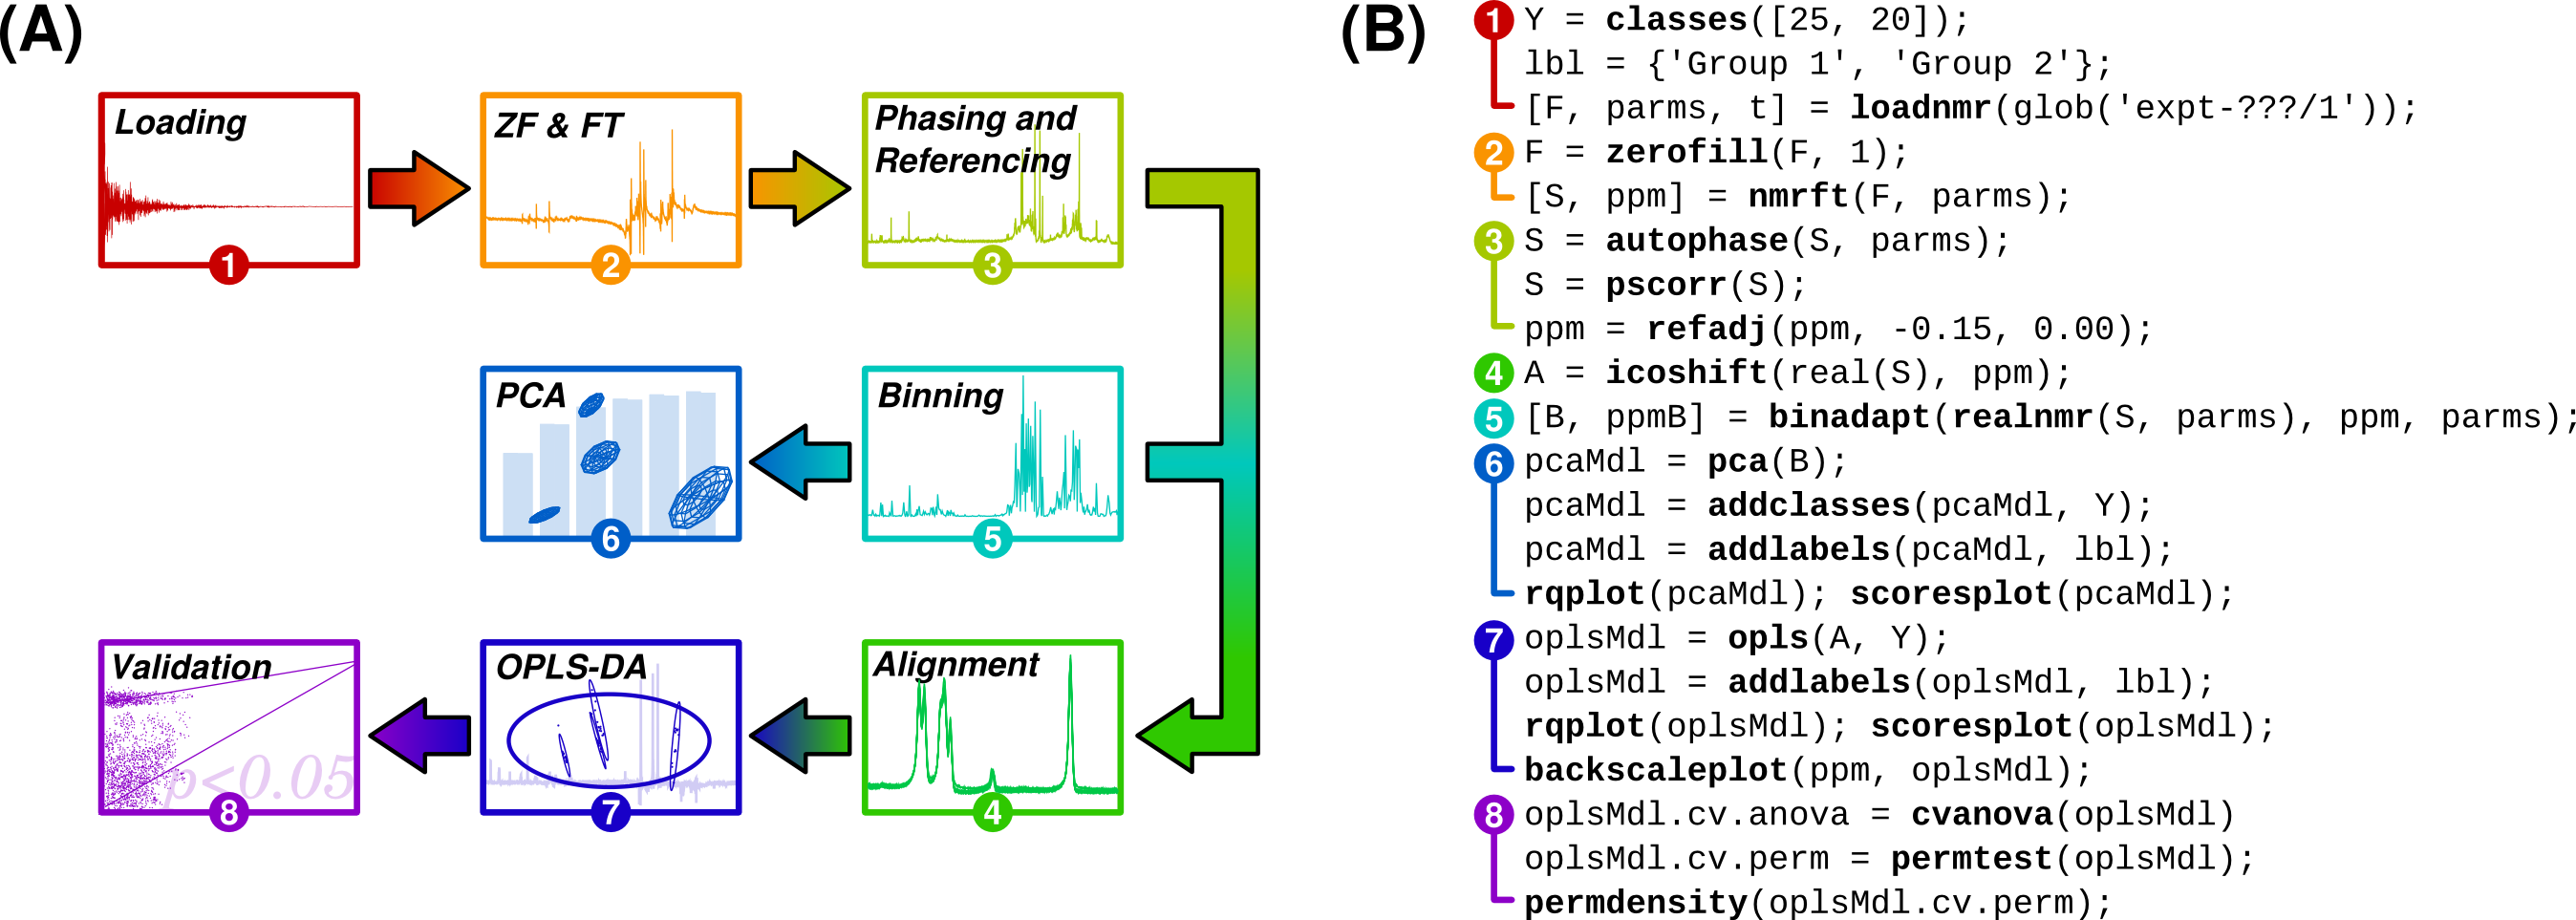
\includegraphics[width=6.5in]{figs/mvapack/01.png}
\end{center}
\caption
      [Example Data Handling Flow in MVAPACK.]{
  {\bf Example Data Handling Flow in MVAPACK.}
  \\
  A general NMR metabolic fingerprinting data handling flow diagram ({\bf A})
  and its associated minimum working example MVAPACK scripts ({\bf B}). This
  minimalistic data handling script is a simple starting point for using
  MVAPACK; much greater flexibility and functionality are present in the
  software than may be shown here. All functions in bold typeface are provided
  in MVAPACK.
}
\end{figure}

\section{Materials and Methods}

\subsection{Software Implementation}

\begin{doublespace}
The MVAPACK software package is written in GNU Octave, an open-source
mathematical programming language that uses MATLAB syntax \cite{eaton2008}.
Every function available in MVAPACK is realized as a single Octave function
file that may be examined or changed using any text editor. Most functions in
MVAPACK follow a similar input-to-output template, where an input data matrix
$\mathbf{A}$ is modified and returned as an output data matrix $\mathbf{B}$.
Other input arguments, required or optional, may accompany $\mathbf{A}$, and
extra output values may accompany $\mathbf{B}$, depending on the specific
needs of the analyst. Models produced by PCA, PLS, OPLS, LDA, MB-PCA and
MB-PLS are all similarly organized into Octave structures (i.e. ``structs'')
that all follow scalar, vector, and matrix notations of Wold et al.
\cite{wold:cils2001}. Thus, functions in MVAPACK are highly modular, often
allowing drop-in replacement of one processing, treatment or modeling method
for another by a simple change of function name and arguments. For instance,
all modeling algorithms allow the specification of a scaling method at the
time they are trained, so all available scaling functions conform to the
same interface: for any input data matrix, a scaled data matrix is returned
alongside the centering and scaling vectors used to compute the matrix.
\\\\
Data may be handled in MVAPACK in either interactive mode, in which the user
types commands into the Octave interpreter one at a time, or in batch mode,
where a complete processing scheme has been laid out in an Octave script to
be executed non-interactively. Once an ideal set of data handling steps is
determined by interactive manipulation of any given dataset, it may be
immortalized in an Octave script, thus providing documentation of procedures
and allowing for rapid recalculation of all associated results.
\\\\
Figure 4.1 illustrates a simple MVAPACK script capable of taking 1D \hnmr{} NMR
data from raw free induction decays to validated PCA and OPLS-DA models. In
section 1, a binary class matrix $\mathbf{Y}$ and an accompanying set of class
labels are built, and the time-domain raw data is loaded into the complex data
matrix $\mathbf{F}$. In section 2, the time-domain data matrix $\mathbf{F}$ is
zero-filled once and Fourier-transformed to produce the complex spectral data
matrix $\mathbf{S}$. Section 3 automatically phase corrects each spectrum in
$\mathbf{S}$, normalizes and corrects for between-spectrum phase differences,
and corrects the chemical shift abscissa to center the reference peak at $0.0$
ppm. In sections 4 and 5, data handling splits into two pathways, where
icoshift alignment \cite{savorani:jmr2010} is used to generate a data matrix
$\mathbf{A}$ fit for full-resolution OPLS-DA and AI-binning
\cite{demeyer:anchem2008} is used to generate a data matrix $\mathbf{B}$ for
PCA. In section 6, a PCA model is built and assigned classes and labels, and
a model quality plot and a scores plot are produced. In section 7, similar
functions are used to train an OPLS-DA model and produce summary plots.
Finally, section 8 performs CV-ANOVA \cite{eriksson:jchemo2008} and response
permutation \cite{westerhuis:metab2008} significance tests to fully validate
the supervised OPLS-DA model. While Figure 4.1 is completely functional, it is
still an extremely bare-bones approach to metabolic fingerprinting. MVAPACK
provides countless other functions and schemes for handling data.
\end{doublespace}

\subsection{Feature Set}

\begin{doublespace}
The functions available in MVAPACK span the following general categories:
data loading and processing (Figure 4.1), treatment (Figure 4.2),
modeling (Figure 4.3), and validation (Figure 4.4) \cite{goodacre:metab2007}.
Specific features in each category are discussed in the following sections.
\end{doublespace}

\begin{table}[h!]
\caption{MVAPACK Processing Feature Matrix.}
\begin{center}
\begin{tabular}{l l | l l l l l l l l l l l l l l l l}
  \hline
  & &
  \rot{Topspin} &
  \rot{VnmrJ} &
  \rot{nmrPipe} &
  \rot{NMRViewJ} &
  \rot{MNova} &
  \rot{ACD/NMR} &
  \rot{Automics} &
  \rot{Chenomx} &
  \rot{KnowItAll} &
  \rot{Metabonomic} &
  \rot{MetaboAnalyst} &
  \rot{AMIX} &
  \rot{SIMCA} &
  \rot{PLS Toolbox} &
  \rot{PyChem} &
  \rot{\bf MVAPACK} \\
  \hline
  \multicolumn{2}{l|}{{\bf Loading}} & & & & & & & & & & & & & & & & \\
  & Bruker, 1D
  & * &   & * & * & * & * & * & * & * & * &   & * &   &   &   & * \\
  & Bruker, 2D
  & * &   & * & * & * & * &   &   &   &   &   &   &   &   &   & * \\
  & Varian, 1D
  &   & * & * & * & * & * & * & * & * &   &   & * &   &   &   & * \\
  \multicolumn{2}{l|}{{\bf Apodization}} & & & & & & & & & & & & & & & & \\
  & Exponential, 1D
  & * & * & * &   & * & * &   & * & * &   &   &   &   &   &   & * \\
  & Exponential, 2D
  & * & * & * &   & * & * &   &   &   &   &   &   &   &   &   & * \\
  & Gaussian, 1D
  & * & * & * &   & * & * &   &   & * &   &   &   &   &   &   & * \\
  & Gaussian, 2D
  & * & * & * &   & * & * &   &   &   &   &   &   &   &   &   & * \\
  & Sine, 1D
  & * & * & * &   & * & * &   &   &   &   &   &   &   &   &   & * \\
  & Sine, 2D
  & * & * & * &   & * & * &   &   &   &   &   &   &   &   &   & * \\
  \multicolumn{2}{l|}{{\bf Zero-filling}} & & & & & & & & & & & & & & & & \\
  & ZF, 1D
  & * & * & * &   & * & * & * & * & * &   &   &   &   &   &   & * \\
  & ZF, 2D
  & * & * & * &   & * & * &   &   &   &   &   &   &   &   &   & * \\
  \multicolumn{2}{l|}{{\bf Transforms}} & & & & & & & & & & & & & & & & \\
  & DFT, 1D
  & * & * & * &   & * & * & * & * & * & * &   &   &   &   &   & * \\
  & DFT, 2D
  & * & * & * &   & * & * &   &   &   &   &   &   &   &   &   & * \\
  & CWT, 1D
  &   &   &   &   & * &   &   &   &   &   &   &   & * &   &   & * \\
  & IST, 2D
  & * & * &   &   & * &   &   &   &   &   &   &   &   &   &   & * \\
  \multicolumn{2}{l|}{{\bf Phase correction}} & & & & & & & & & & & & & & & & \\
  & Manual, 1D
  & * & * & * &   & * & * & * & * & * & * &   & * &   &   &   & * \\
  & Manual, 2D
  & * & * & * &   & * & * &   &   &   &   &   & * &   &   &   & * \\
  & Automatic, 1D
  & * & * &   &   & * & * & * & * & * &   &   & * &   &   &   & * \\
  & Automatic, 2D
  & * & * &   &   & * & * &   &   &   &   &   &   &   &   &   & *
\end{tabular}
\end{center}
\end{table}

\subsubsection{Processing}

\begin{doublespace}
Loading of Bruker raw data is available using either a high-performance
DMX-format loading routine or nmrPipe \cite{delaglio:jbnmr1995} as a backend,
and loading of Varian data is available using an nmrPipe backend. Additionally,
data in a variety of structured text formats may be read into MVAPACK using
standard GNU Octave routines. The NMR spectral processing functions in MVAPACK
follow the traditional paradigms of NMR processing \cite{hoch1996} and include
methods for apodization, zero-filling, Fourier transformation, Iterative Soft
Thresholding (IST) reconstruction \cite{hyberts:jacs2007}, manual and automatic
phase correction
\cite{siegel:aca1981,chen:jmr2002,balacco:mrc2009}, region of interest
selection and manipulation, peak picking \cite{du:binf2006}, integration and
referencing.
\end{doublespace}

\begin{table}[h!]
\caption{MVAPACK Treatment Feature Matrix.}
\begin{center}
\begin{tabular}{l l | l l l l l l l l l l l l l l l l}
  \hline
  & &
  \rot{Topspin} &
  \rot{VnmrJ} &
  \rot{nmrPipe} &
  \rot{NMRViewJ} &
  \rot{MNova} &
  \rot{ACD/NMR} &
  \rot{Automics} &
  \rot{Chenomx} &
  \rot{KnowItAll} &
  \rot{Metabonomic} &
  \rot{MetaboAnalyst} &
  \rot{AMIX} &
  \rot{SIMCA} &
  \rot{PLS Toolbox} &
  \rot{PyChem} &
  \rot{\bf MVAPACK} \\
  \hline
  \multicolumn{2}{l|}{{\bf Binning}} & & & & & & & & & & & & & & & & \\
  & Uniform, 1D
  &   &   &   &   & * & * & * &   & * & * &   & * &   &   &   & * \\
  & Uniform, 2D
  &   &   &   &   &   & * & * &   & * &   &   & * &   &   &   & * \\
  & Optimized, 1D
  &   &   &   &   &   &   &   &   &   &   &   & * &   &   &   & * \\
  & Adaptive, 1D
  &   &   &   &   &   &   &   &   &   &   &   & * &   &   &   & * \\
  & Adaptive, 2D
  &   &   &   &   &   &   &   &   &   &   &   &   &   &   &   & * \\
  \multicolumn{2}{l|}{{\bf Alignment}} & & & & & & & & & & & & & & & & \\
  & Global
  &   &   &   &   &   &   & * &   &   &   &   &   &   &   &   & * \\
  & Interval
  &   &   &   &   &   &   & * &   &   &   &   &   &   &   &   & * \\
  \multicolumn{2}{l|}{{\bf Normalization}} & & & & & & & & & & & & & & & & \\
  & CS
  &   &   &   &   &   &   &   &   &   &   & * & * &   & * & * & * \\
  & PQ
  &   &   &   &   &   &   &   &   &   &   & * &   &   &   &   & * \\
  & HM
  &   &   &   &   &   &   &   &   &   &   &   &   &   &   &   & * \\
  & SNV
  &   &   &   &   &   &   & * &   & * & * &   & * &   & * & * & * \\
  & MSC
  &   &   &   &   &   &   & * &   & * &   &   &   &   & * & * & * \\
  & PSC
  &   &   &   &   &   &   &   &   &   &   &   &   &   &   &   & * \\
  \multicolumn{2}{l|}{{\bf Scaling}} & & & & & & & & & & & & & & & & \\
  & UV
  &   &   & * &   &   &   & * &   & * & * & * & * & * & * & * & * \\
  & Pareto
  &   &   &   &   & * &   & * &   & * & * & * &   & * &   &   & * \\
  & Range
  &   &   &   &   & * &   &   &   & * & * & * &   & * &   &   & * \\
  & Level
  &   &   &   &   & * &   &   &   &   &   &   &   & * &   &   & * \\
  & VAST
  &   &   &   &   & * &   &   &   & * &   &   &   & * &   &   & *
\end{tabular}
\end{center}
\end{table}

\subsubsection{Treatment}

\begin{doublespace}
Functions for statistical data treatment in MVAPACK include binning
\cite{sousa:cils2013,demeyer:anchem2008}, alignment \cite{savorani:jmr2010},
normalization \cite{barnes:aspec1989,dieterle:anchem2006,torgrip:metab2008},
scaling \cite{vandenberg:bmcg2006}, and direct orthogonal signal correction
\cite{westerhuis:cils2001}. In addition, MVAPACK supports uniform binning
and AI-binning (cf. Chapter 6) of third-order data tensors stored as arrays
of real matrices in Octave.
\end{doublespace}

\begin{table}[h!]
\caption{MVAPACK Modeling Feature Matrix.}
\begin{center}
\begin{tabular}{l l | l l l l l l l l l l l l l l l l}
  \hline
  & &
  \rot{Topspin} &
  \rot{VnmrJ} &
  \rot{nmrPipe} &
  \rot{NMRViewJ} &
  \rot{MNova} &
  \rot{ACD/NMR} &
  \rot{Automics} &
  \rot{Chenomx} &
  \rot{KnowItAll} &
  \rot{Metabonomic} &
  \rot{MetaboAnalyst} &
  \rot{AMIX} &
  \rot{SIMCA} &
  \rot{PLS Toolbox} &
  \rot{PyChem} &
  \rot{\bf MVAPACK} \\
  \hline
  \multicolumn{2}{l|}{{\bf Bilinear}} & & & & & & & & & & & & & & & & \\
  & PCA
  &   &   & * &   & * &   & * &   & * & * & * & * & * & * & * & * \\
  & LDA
  &   &   &   &   &   &   & * &   &   &   &   & * &   &   &   & * \\
  & PLS
  &   &   &   &   &   &   & * &   &   & * & * & * & * & * &   & * \\
  & OPLS
  &   &   &   &   &   &   &   &   &   &   &   &   & * & * &   & * \\
  \multicolumn{2}{l|}{{\bf Multiblock}} & & & & & & & & & & & & & & & & \\
  & MB-PCA
  &   &   &   &   &   &   &   &   &   &   &   &   &   & * &   & * \\
  & MB-PLS
  &   &   &   &   &   &   &   &   &   &   &   &   &   & * &   & *
\end{tabular}
\end{center}
\end{table}

\subsubsection{Modeling}

\begin{doublespace}
MVAPACK provides complete support for building PCA \cite{jolliffe2002},
LDA \cite{hardle2012}, PLS \cite{wold1993,geladi:aca1986,wold:cils2001},
OPLS \cite{trygg:jchemo2002,bylesjo:jchemo2006}, MB-PCA and MB-PLS
\cite{westerhuis:jchemo1998,smilde:jchemo2003} models from processed
and treated datasets. At the current time, only bilinear factorizations
are supported within MVAPACK.
\end{doublespace}

\begin{table}[h!]
\caption{MVAPACK Validation Feature Matrix.}
\begin{center}
\begin{tabular}{l l | l l l l l l l l l l l l l l l l}
  \hline
  & &
  \rot{Topspin} &
  \rot{VnmrJ} &
  \rot{nmrPipe} &
  \rot{NMRViewJ} &
  \rot{MNova} &
  \rot{ACD/NMR} &
  \rot{Automics} &
  \rot{Chenomx} &
  \rot{KnowItAll} &
  \rot{Metabonomic} &
  \rot{MetaboAnalyst} &
  \rot{AMIX} &
  \rot{SIMCA} &
  \rot{PLS Toolbox} &
  \rot{PyChem} &
  \rot{\bf MVAPACK} \\
  \hline
  \multicolumn{2}{l|}{{\bf Validation}} & & & & & & & & & & & & & & & & \\
  & \rsq{}, \qsq{}
  &   &   &   &   &   &   & * &   & * & * & * & * & * & * & * & * \\
  & Permutation
  &   &   &   &   &   &   &   &   &   &   & * &   & * & * &   & * \\
  & CV-ANOVA
  &   &   &   &   &   &   &   &   &   &   &   &   & * &   &   & * \\
  \multicolumn{2}{l|}{{\bf Visualization}} & & & & & & & & & & & & & & & & \\
  & 2D Scores
  &   &   &   &   & * &   & * &   & * & * & * & * & * & * & * & * \\
  & 3D Scores
  &   &   &   &   &   &   &   &   & * & * & * &   & * & * &   & * \\
  & Loadings
  &   &   &   &   & * &   & * &   & * & * & * & * & * & * & * & * \\
  & Backscaling
  &   &   &   &   &   &   &   &   &   &   &   &   &   &   &   & * \\
  & S-plot
  &   &   &   &   &   &   &   &   &   &   &   &   & * &   &   & * \\
  & SUS-plot
  &   &   &   &   &   &   &   &   &   &   &   &   & * &   &   & * \\
  & Data Ellipsoid
  &   &   &   &   &   &   &   &   &   & * & * & * & * & * &   & * \\
  & Class Ellipsoid
  &   &   &   &   &   &   &   &   &   &   &   &   &   &   &   & *
\end{tabular}
\end{center}
\end{table}

\subsubsection{Validation}

\begin{doublespace}
All PCA and MB-PCA models are validated as they are built based on the results
of a leave-one-out internal cross-validation
\cite{eastment:tech1982,eshghi:cils2014}, and all PLS, OPLS and MB-PLS models
are validated during training based on results of a Monte Carlo leave-$n$-out
internal cross-validation \cite{xu:cils2001,xu:jchemo2004}. In all cases, a
set of \rsq{} (i.e. \rsqx{} and \rsqy{}) statistics are generated to assess
how well each data and response matrix is approximated by the models, and
\qsq{} statistics are generated to describe self-consistency and predictive
ability of each data matrix in PCA and PLS models, respectively. Per-component
\rsq{} and \qsq{} statistics are utilized by MVAPACK to estimate the optimal
number of model components. Further validation of supervised models is
available in the form of CV-ANOVA \cite{eriksson:jchemo2008} and response
permutation \cite{westerhuis:metab2008} significance testing, both of which
report $p$ values that indicate model validity.
\end{doublespace}

\section{Discussion and Conclusions}

\begin{doublespace}
This chapter presents MVAPACK, a completely free and open-source data handling
environment tailor-suited to NMR chemometrics and \hnmr{} NMR and MS metabolic
fingerprinting applications. Unlike data handling chains composed of multiple
commercial software packages, MVAPACK is free to use, modify and distribute
according to the GNU General Public License \cite{gpl3} and provides a single
consistent data handling environment. Because MVAPACK is written for GNU
Octave, researchers already familiar with MATLAB syntax will also be familiar
with MVAPACK without a considerable learning curve. Datasets and results
obtained using MVAPACK are readily saved and exhanged using GNU Octave built-in
support for the MATLAB {\it mat}-file format.
\\\\
A recent review \cite{izquierdo:pnmrs2011} of software packages targeted at
metabolomics highlights the piecemeal nature of 1D \hnmr{} NMR data handling
in the field, where no single package is capable of performing all the tasks
required by the analyst. MVAPACK addresses this need by providing a complete
pipeline that is tuned for metabolic fingerprinting. Use of MVAPACK reduces
data analysis time in metabolic fingerprinting from days to minutes, simply
by collecting all the required functions into a single scriptable environment.
In fact, the example script in Figure 4.1 would execute in under five minutes
on a modern GNU/Linux or Mac OS X computer system.
\\\\
The routine processing of {\it any} 1D and 2D NMR spectral data may be readily
done with MVAPACK, and processing routines are easily batched. The MVAPACK
scripts written to analyze the datasets in \hyperlink{chapter.3}{Chapter 3}
are composed of intuitive, modular commands that logically subdivide the script
into recognizable tasks like automatic phase correction, spectral alignment,
normalization, {\it etc}. Furthermore, aside from physical memory limitations
of the host computer, MVAPACK does not impose any limit on the number of NMR
observations that may be simultaneously handled.
\\\\
A major advantage of MVAPACK is the seamless transfer of the processed, treated
NMR data to multivariate statistical analyses. The PCA, PLS, OPLS and LDA
bilinear modeling algorithms, now ubiquitous in the metabolomics community,
are all implemented in MVAPACK using a consistent under-the-hood framework.
Model results may be visualized and interpreted using MVAPACK routines that
provide scatter, line and bar plots of model scores, loadings and validation
statistics. Critically, MVAPACK automatically ensures that {\it all} trained
models are valid using leave-one-out and Monte Carlo leave-$n$-out internal
cross-validation routines and provides further means of validating supervised
models in the form of CV-ANOVA and response permutation significance testing.
Several powerful examples of MVAPACK applied to real datasets are presented in
\hyperlink{chapter.3}{Chapter 3}. Because it implements well-established
algorithms available from peer-reviewed chemometrics literature, MVAPACK
generates identical results when compared to expensive software packages
like Umetrics SIMCA-P+.
\\\\
In short, MVAPACK provides a complete platform for NMR chemometric data
handling that is ideal for both routine handling of metabolomics datasets and
development of novel algorithms. Unlike its closed-source predecessors, the
modular, open-source design of MVAPACK readily accepts new functionality,
allowing it to grow and maintain pace with the state-of-the-art in the
chemometrics literature. MVAPACK is freely available for download at
\url{http://bionmr.unl.edu/mvapack.php}. Detailed documentation of MVAPACK,
all datasets presented in \hyperlink{chapter.3}{Chapter 3}, and the scripts
used to handle them are also available for download.
\end{doublespace}

\bibliographystyle{abbrv}
\bibliography{bworley}



\chapter{Phase-Scatter Correction of NMR Datasets}

\section{Introduction}

\begin{doublespace}
Normalization applied directly to hypercomplex NMR data (or its real component)
is sub-optimal, as even small phase differences between observations can
frustrate the estimation of normalization factors
(See \hyperlink{section.3.3}{Section 3.3}). Possibly worse, blind
normalization of poorly phased spectral data can accentuate experimentally
irrelevant spectral features in a data tensor during multivariate modeling,
leading the analyst to erroneous conclusions. These difficulties motivated
the development of phase-scatter correction (PSC, \cite{worley:abio2013}) as
a means of simultaneously correcting the coupled phase errors and dilution
errors that are present in hypercomplex NMR data tensors.
\end{doublespace}

\subsection{Metabolomics}

\begin{doublespace}
FIXME.
\end{doublespace}

\subsection{High-throughput Screening}

\begin{doublespace}
FIXME.
\end{doublespace}

\section{Theory}

\subsection{Multiplicative Scatter Correction}

\begin{doublespace}
Phase-scatter correction (PSC) is effectively an extension of multiplicative
scatter correction (MSC) to handle phase errors during normalization. In MSC,
each real spectrum is scaled around its mean intensity and shifted to match a
reference spectrum, typically the mean of the dataset \cite{fearn:cils2009}.
Optimal normalization factors ($\mathbf{b}$) of a data matrix $\mathbf{X}$ are
determined by a linear regression of the mean-centered reference vector onto
the mean-centered matrix:

\begin{equation}
\big( \mathbf{X} - \langle \mathbf{X} \rangle \big)^T \mathbf{b}
 = \big( \mathbf{r} - \langle \mathbf{r} \rangle \big)^T
\end{equation}

where observations are stored as row vectors in $\mathbf{X}$, and $\mathbf{r}$
is the reference observation row vector. The equation above represents an
overdetermined system of linear equations, therefore the least-squares estimate
of $\mathbf{b}$ may be computed rapidly, and MSC is rather computationally
efficient.
\end{doublespace}

\subsection{Phase-scatter Correction}

\begin{doublespace}
PSC additionally corrects zero- and first-order phase errors during
normalization, requiring a nonlinear optimization of the following objective:

\begin{equation}
Q(\mathbf{X} \mid \mathbf{p})
 = \sum_{n=1}^N \| \mathbf{z}_n \circ \mathbf{x}_n - \mathbf{r} \|_2^2
\end{equation}

where $\circ$ denotes the element-wise product, the mean-centered matrix
$\mathbf{X}$ lies in $\mathbb{H}_1^{N \times K}$, the mean-centered reference
$\mathbf{r}$ lies in $\mathbb{H}_1^K$, and the set of parameters $\mathbf{p}$
includes a normalization factor and two phase errors per observation
in $\mathbf{X}$:

\begin{equation}
\mathbf{p} = \{
  b_1, \dots b_N,
  \theta_{0,1}, \dots \theta_{0,N},
  \theta_{1,1}, \dots \theta_{1,N} \}
\end{equation}

and each vector $\mathbf{z}_n$ contains the normalization and phase corrections
for the $n$-th observation $\mathbf{x}_n$:

\begin{equation}
z_{n,k} = b_n e^{u_1 (\theta_{0,n} + \theta_{1,n} k)}
\end{equation}

Because the reference observation $\mathbf{r}$ is fixed during optimization,
minimization of $Q(\mathbf{X} \mid \mathbf{p})$ may be achieved by
independently minimizing each observation's contributions. Minimization is
carried out for every observation in the data matrix using Levenberg-Marquardt
nonlinear least squares \cite{marquardt:jsiam1963} as implemented by the
{\it leasqr} function in GNU Octave, a function similar to MATLAB's
{\it nlinfit}. Each corrected spectrum $\hat{\mathbf{x}}_n$ is then returned
from optimization as follows:

\begin{equation}
\hat{\mathbf{x}}_n
 = \mathbf{z}_n \circ \mathbf{x}_n
 + \langle \mathbf{r} \rangle
\end{equation}

Phase-scatter correction of 50 1D \hnmr{} NMR spectra having 32$k$ complex
points each requires approximately 30 seconds on a single-core 3.2 GHz Intel
workstation running GNU Octave 3.6.
\end{doublespace}

\subsection{Ensemble Phase Correction}

\begin{doublespace}
It is important recognize that the phase-scatter correction objective function
$Q(\mathbf{X} \mid \mathbf{p})$ provides no measure of ideal phase values,
meaning that PSC requires an additional phase correction step prior to its
execution in order to ensure adequate initial conditions. Even when
$\mathbf{X}$ has been suitably phase-corrected, PSC may still attempt to
minimize scatter between spectra by re-introducing phase errors. This
undesirable behavior of PSC may be observed when large disparities in
spectral intensities are present between observations. To correct this,
a standard phase correction objective
$f : \mathbb{H}_D^{K} \to \mathbb{R}$ may be combined with
the PSC objective using a Lagrange multiplier, like so:

\begin{equation}
\Lambda(\mathbf{X} \mid \mathbf{p}) =
 -\sum_{n=1}^N f(\boldsymbol{\theta}_n \circ \mathbf{x}_n) +
 \lambda \sum_{n=1}^N \| \mathbf{z}_n \circ \mathbf{x}_n -
            \langle \mathbf{Z} \circ \mathbf{X} \rangle \|_2^2
\end{equation}

where the correction matrix $\mathbf{Z}$ has the same form as in PSC, expressed
as a real diagonal matrix of normalization factors $\mathbf{B}$ and a
hypercomplex matrix of phase factors $\mathbf{\Theta}$:

\begin{equation}
\mathbf{Z} = \mathbf{B} \mathbf{\Theta}
\end{equation}

and $\boldsymbol{\theta}_n$ is the $n$-th row of $\mathbf{\Theta}$. The new
ensemble phase correction (EPC) objective function
$\Lambda(\mathbf{X} \mid \mathbf{p})$ balances the potentially opposing goals
of phase correction and scatter correction through the Lagrange multiplier
$\lambda$, and does not require the specification of a reference observation
$\mathbf{r}$. In effect, EPC allows its scatter correction reference to float
as the current mean of the data, $\langle \mathbf{Z} \circ \mathbf{X} \rangle$.
This floating reference requires the simultaneous optimization of all the
parameters in $\mathbf{p}$, unlike phase-scatter correction. Efficient
minimization of $\Lambda(\mathbf{X} \mid \mathbf{p})$ may be accomplished by
a modified Nelder-Mead simplex optimization procedure \cite{nelder:compj1964},
which serially updates the simplices of all observations at each global
iteration and maintains the current mean vector
$\langle \mathbf{Z} \circ \mathbf{X} \rangle$ at each update.
\\\\
In contrast to phase-scatter correction, which seeks to minimize the scatter
of data matrix observations around a fixed reference, ensemble phase correction
approaches the dilemma of entwined phase and normalization errors from an
opposing direction by introducing a scatter term into a standard automatic
phase correction procedure. The amount of normalization achieved by EPC is
directly controlled by the magnitude of $\lambda$: in the opposite limits of
$\lambda = 0$ and $\lambda \to \infty$, EPC becomes equivalent to standard
phase correction and phase-scatter correction with a floating reference,
respectively.
\end{doublespace}

\section{Materials and Methods}

\begin{doublespace}
FIXME.
\end{doublespace}

\section{Results}

\begin{doublespace}
FIXME.
\end{doublespace}

\section{Discussion}

\begin{doublespace}
FIXME.
\end{doublespace}

\section{Conclusions}

\begin{doublespace}
FIXME.
\end{doublespace}

\bibliographystyle{abbrv}
\bibliography{bworley}



\chapter{Generalized Adaptive Intelligent Binning of Multiway Data}

\begin{quote}
{\it
  The art of doing mathematics consists in finding that special case which
  contains all the germs of generality.}
\\\\
 -- David Hilbert
\end{quote}

\section{Introduction}

\begin{figure}[hb!]
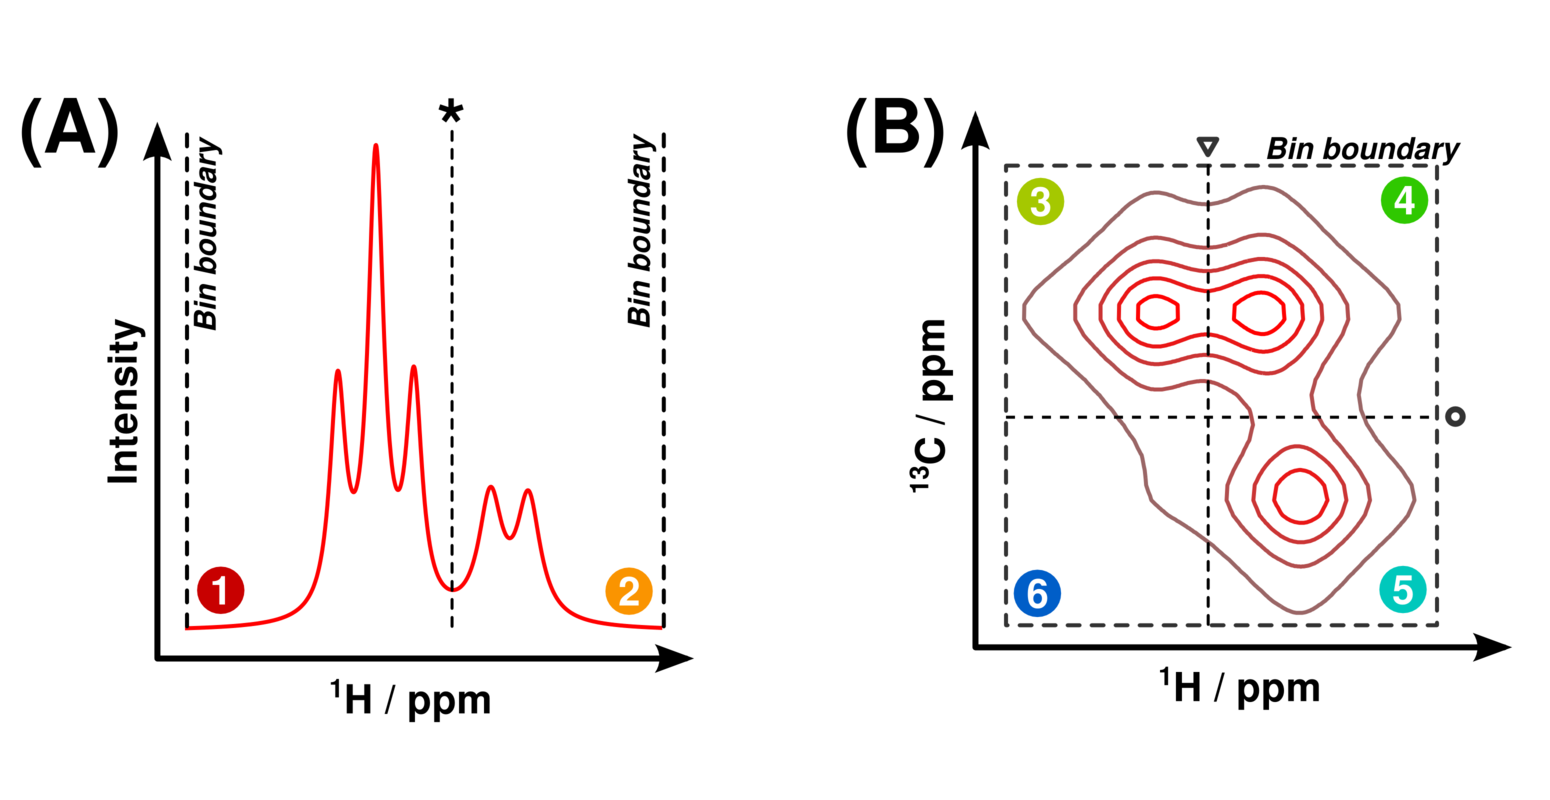
\includegraphics[width=6.5in]{figs/gaibin/01.png}
\caption
      [Generalization of Adaptive Intelligent Binning.]{
  {\bf Generalization of Adaptive Intelligent Binning.}
  \\
  ({\bf A}) In the one-dimensional case, the bin containing regions 1 and 2
  is optimally subdivided ({\it asterisk}) when the sum of the objective values
  in regions 1 and 2 is maximal and greater than the original bin's objective
  value. ({\bf B}) In the $D$-dimensional case, there are now $D$ possible
  dimensions along which an optimal subdivision may exist. The optimal
  subdivision along the \hnmr{} dimension ({\it triangle}) occurs when the sum
  of the objective values in regions 3+6 and 4+5 is maximal and greater than
  that of the original bin. Similarly, the optimal subdivision along the
  \cnmr{} dimension ({\it circle}) occurs when the sum of the objective values
  in regions 3+4 and 5+6 is maximal and above the original bin objective. A
  comparison between all possible optimal subdivisions along all dimensions
  yields the best possible subdivision (\cnmr{}, {\it circle}).
}
\end{figure}

\begin{doublespace}
By and large, the phase ``NMR metabolic fingerprinting'' implies the use of
one-dimensional (1D) \hnmr{} NMR spectroscopic methods, due in no small part
to the ease and speed of 1D data collection and the large natural abundance
of NMR-active protons found in metabolomics samples
\cite{lindon:cmr2000,worley:cmb2013}. Before processed spectra are
submitted to PCA or PLS for modeling, they are often subdivided into bins
to simplify multivariate analyses. Spectral binning, introduced and described
in detail in \hyperlink{chapter.3}{Chapter 3}, reduces the dimensionality of
a data matrix and masks chemical shift variability between samples at the
expense of decreased model interpretability: any given bin in a 1D \hnmr{} NMR
spectral dataset may contain several overlapped signals from multiple distinct
metabolites \cite{aberg:abc2009}. Thus, without utilizing
computationally intensive methods of deconvolution to tease apart signal
contributions from individual metabolites
\cite{astle:jasa2012,zheng:binf2011}, the resulting fingerprint from a
binned 1D dataset is usually limited to high-level inference about metabolic
trends.
\\\\
By leveraging the connectivities between \hnmr{} and \cnmr{} nuclei in
metabolites, two-dimensional (2D) heteronuclear NMR methods reduce spectral
overlap by spreading \hnmr{} information over a second (\cnmr) chemical shift
dimension \cite{mandal:cmr2004}. Heteronuclear single quantum coherence (HSQC)
experiments are commonly performed in NMR metabolic profiling studies, and
provide an NMR singlet or multiplet for each directly bonded \hcnmr{} pair
in the sample. Developments in NMR hardware and acquisition techniques have
brought natural abundance \hcnmr{} HSQC experiment times down to values
compatible with high-throughput metabolic fingerprinting studies
\cite{motta:anchem2010,rai:anchem2012}. However, multivariate analysis
of 2D NMR datasets is still a nontrivial undertaking that requires either
vectorization \cite{hedenstrom:cils2008}, which breaks the inherent
structure of the data, or the use of multilinear factorizations
\cite{lu:ieee2009,lu:pr2011}, which are more computationally intensive
and difficult to cross-validate.
\\\\
Spectral binning is another potential means of preparing 2D NMR datasets for
multivariate analysis that holds several advantages over binning 1D spectra.
First, multiple integration of bins maps each spectrum to an observation
vector regardless of its original dimensionality, allowing bilinear PCA and
PLS algorithms to be used without concern for loss of the inherent structure
of the data. Second, binning of 2D spectral data yields more well-conditioned
data matrices than simple vectorization. Finally, because signals are better
resolved in 2D spectra, each bin contains substantially fewer signals from
distinct metabolites. Multiple different algorithms have been developed to
bin 1D NMR data \cite{
  anderson:metab2008,
  anderson:metab2011,
  davis:cils2007,
  demeyer:anchem2008,
  sousa:cils2013}, and the use of uniform binning on 2D NMR data has also been
reported \cite{van:jpr2008}. However, to our knowledge, no methods
exist to {\it intelligently} bin multidimensional data for use in multivariate
analyses. This motivated the development of a generalization of Adaptive
Intelligent (AI) binning \cite{demeyer:anchem2008} to spectral data
of any dimensionality, called Generalized Adaptive Intelligent (GAI) binning
(Figure 6.1).
\end{doublespace}

\section{Theory}

\subsection{AI-binning}

\begin{doublespace}
Generalized AI-binning (GAI-binning) is a logical extension of AI-binning to
two or more dimensions. In the AI algorithm (Figure 6.1A), bins are recursively
subdivided until a stopping criterion or minimum bin width is reached
\cite{demeyer:anchem2008}. For a 1D dataset containing $N$ spectra,
the following objective function is used to assess the quality of each bin:

\begin{equation}
V_b = \frac{1}{N}
  \sum_{n=1}^N \left[
    (max_{n,b} - I_{n,b,1})
    (max_{n,b} - I_{n,b,end}) \right]^\frac{R}{2}
\end{equation}

where $max_{n,b}$ is the maximum intensity inside the bin $b$ in spectrum $n$,
and $I_{n,b,1}$ and $I_{n,b,end}$ are the bin edge intensities. The exponent
$R$ in the AI objective function is referred to as a `resolution parameter',
which offers a means of tuning the binning result based on signal-to-noise and
peak resolution of a dataset. The replacement of $R$ with $\frac{R}{2}$ in the
exponent of equation 6.1, enables a slightly modified interpretation of each
summed term in the AI objective function as a relaxed form of a geometric mean
of the differences between the bin edge intensities and the maximum bin
intensity. At each subdivision step, new bin edges are chosen to maximize the
combined (summed) objective values of the two resulting bins over the objective
value of the original bin. If no bin subdivision exists with a combined
objective value greater than that of the original bin, recursive subdivision
within that bin is terminated, and the AI algorithm terminates once all bins
may no longer be subdivided.
\end{doublespace}

\subsection{GAI-binning}

\begin{doublespace}
In two or more dimensions, the set of bin boundary points expands to include
all points that lie on the edges (or faces, hyperfaces, {\it etc.}) of the bin.
By denoting the set of all edge points in bin $b$ as $E_b$, a new objective
function may be constructed:

\begin{equation}
V_b = \frac{1}{N}
  \sum_{n=1}^N \left[
    \prod_{e \in E_b} (max_{n,b} - I_e)
  \right]^\frac{R}{||E_b||}
\end{equation}

Thus, the GAI algorithm computes the `relaxed' geometric mean of the
differences between the bin maximum and all points on the boundary. In the
case of one-dimensional data, it is apparent that equation 6.2 reduces to
equation 6.1, and GAI-binning operates identically to AI-binning. As
dimensionality increases, the risk of floating-point overflow or underflow
increases due to the larger bin edge set $E_b$. To avoid this, the following
`log-objective' may be used in lieu of equation 6.2:

\begin{equation}
V_{b,ln} = \frac{R}{N ||E_b||}
  \sum_{n=1}^N \sum_{e \in E_b}
    \ln(max_{n,b} - I_e)
\end{equation}

Like AI-binning, GAI-binning initializes a bin around the entire dataset and
proceeds to recursively subdivide each bin until a minimum bin size is reached
or no bin may be divided to yield an increase in the objective value. Because
the number of ways to subdivide each bin increases with dimensionality, all
possible dimensions are tested, and the new bin boundary that maximizes the
objective over all possible subdivision dimensions is selected (Figure 6.1B).
Therefore, the GAI algorithm may be considered a form of binary space
partitioning (BSP) which limits its partition hyperplanes to lying orthogonally
to the basis vectors of the coordinate system \cite{deberg2000}.
\end{doublespace}

\subsection{Noise Bin Elimination}

\begin{doublespace}
It is important that noise bins be removed from the data matrix prior to
multivariate analysis, as their presence is known to negatively impact the
interpretability and reliability of multivariate models
\cite{halouska:jmr2006,bro:anmeth2014}. Because the integration of a
noisy space of increasing dimensionality ({\it i.e.} double or triple
integration) results in a random variable having a similarly increasing
variance, the importance of noise removal is compounded in multidimensional
binning. Therefore, a noise bin removal step based on spectral intensity was
added to the GAI algorithm. A running mean and variance calculation was
performed to estimate the noise floor of each spectrum. The initial mean
$\mu_n$ and standard deviation $\sigma_n$ of the noise were computed using the
first 32 points on one edge of the spectrum, which were assumed to contain only
baseline noise. Every other data point was then classified as signal or noise
based on whether its intensity exceeded the current running noise floor,
$\mu_n + 3 \sigma_n$. Upon inclusion of a new noise data point, the mean and
standard deviation of the noise were appropriately updated. Once the estimated
noise floor was determined for each spectrum in the dataset, a threshold for
bin removal was computed as the median noise floor of all the spectra:

\begin{equation}
I_{th} = \mathrm{med}_n (\mu_n + k \sigma_n)
\end{equation}

where $k$ is a user-selectable parameter to adjust the noise threshold. Only
bins whose maximum intensity fell above $I_{th}$ were retained in the final
data matrix.
\end{doublespace}

\section{Materials and Methods}

\subsection{Human Liver Dataset}

\begin{doublespace}
Two independently collected \hcnmr{} HSQC NMR datasets from ongoing
metabolomics studies were used as test cases for the GAI-binning algorithm.
For the first dataset, twenty-four 1.0 mL samples of SK-Hep1 human liver cells
were provided for metabolic fingerprinting, half of which were treated with
50 $\mu$M tetrathiomolybdate (TTM). The cells were extracted into 80:20
methanol:water to collect the water-soluble metabolites, spun in a rotary
evaporator for two hours, lyophilized at -50 $^\circ$C and 0.02 mBar for 24
hours, and finally redissolved in 600 $\mu$L of 50.0 mM phosphate buffer in
99.8\% D$_2$O (Isotec, St. Louis, MO) adjusted to pH 7.4. The redissolved,
pH-adjusted samples were then collected into NMR tubes.
\\\\
Experiments were collected on a Bruker Avance III HD 700 MHz spectrometer
equipped with a 5 mm inverse quadruple-resonance (\hnmr{}, \cnmr{}, \nnmr{},
\pnmr{}) cryoprobe with cooled \hnmr{} and \cnmr{} channels and a {\it z}-axis
gradient. A Bruker SampleJet and ICON-NMR were used to automate NMR data
collection. A 2D gradient-enhanced \hcnmr{} HSQC with improved sensitivity
\cite{palmer:jmr1991,kay:jacs1992} ({\it hsqcetgpsi}) was collected for
each sample. Spectra were collected with 4 scans and 16 dummy scans over a
uniform Nyquist grid of 512 and 64 complex points along the \hnmr{} and \cnmr{}
dimensions, respectively. Spectral windows were set to 3,285 $\pm$ 4,545 Hz
along \hnmr{} and 12,677 $\pm$ 14,620 Hz along \cnmr{}. All spectra were
collected at a sample temperature of 298.0 K.
\end{doublespace}

\begin{figure}[hb!]
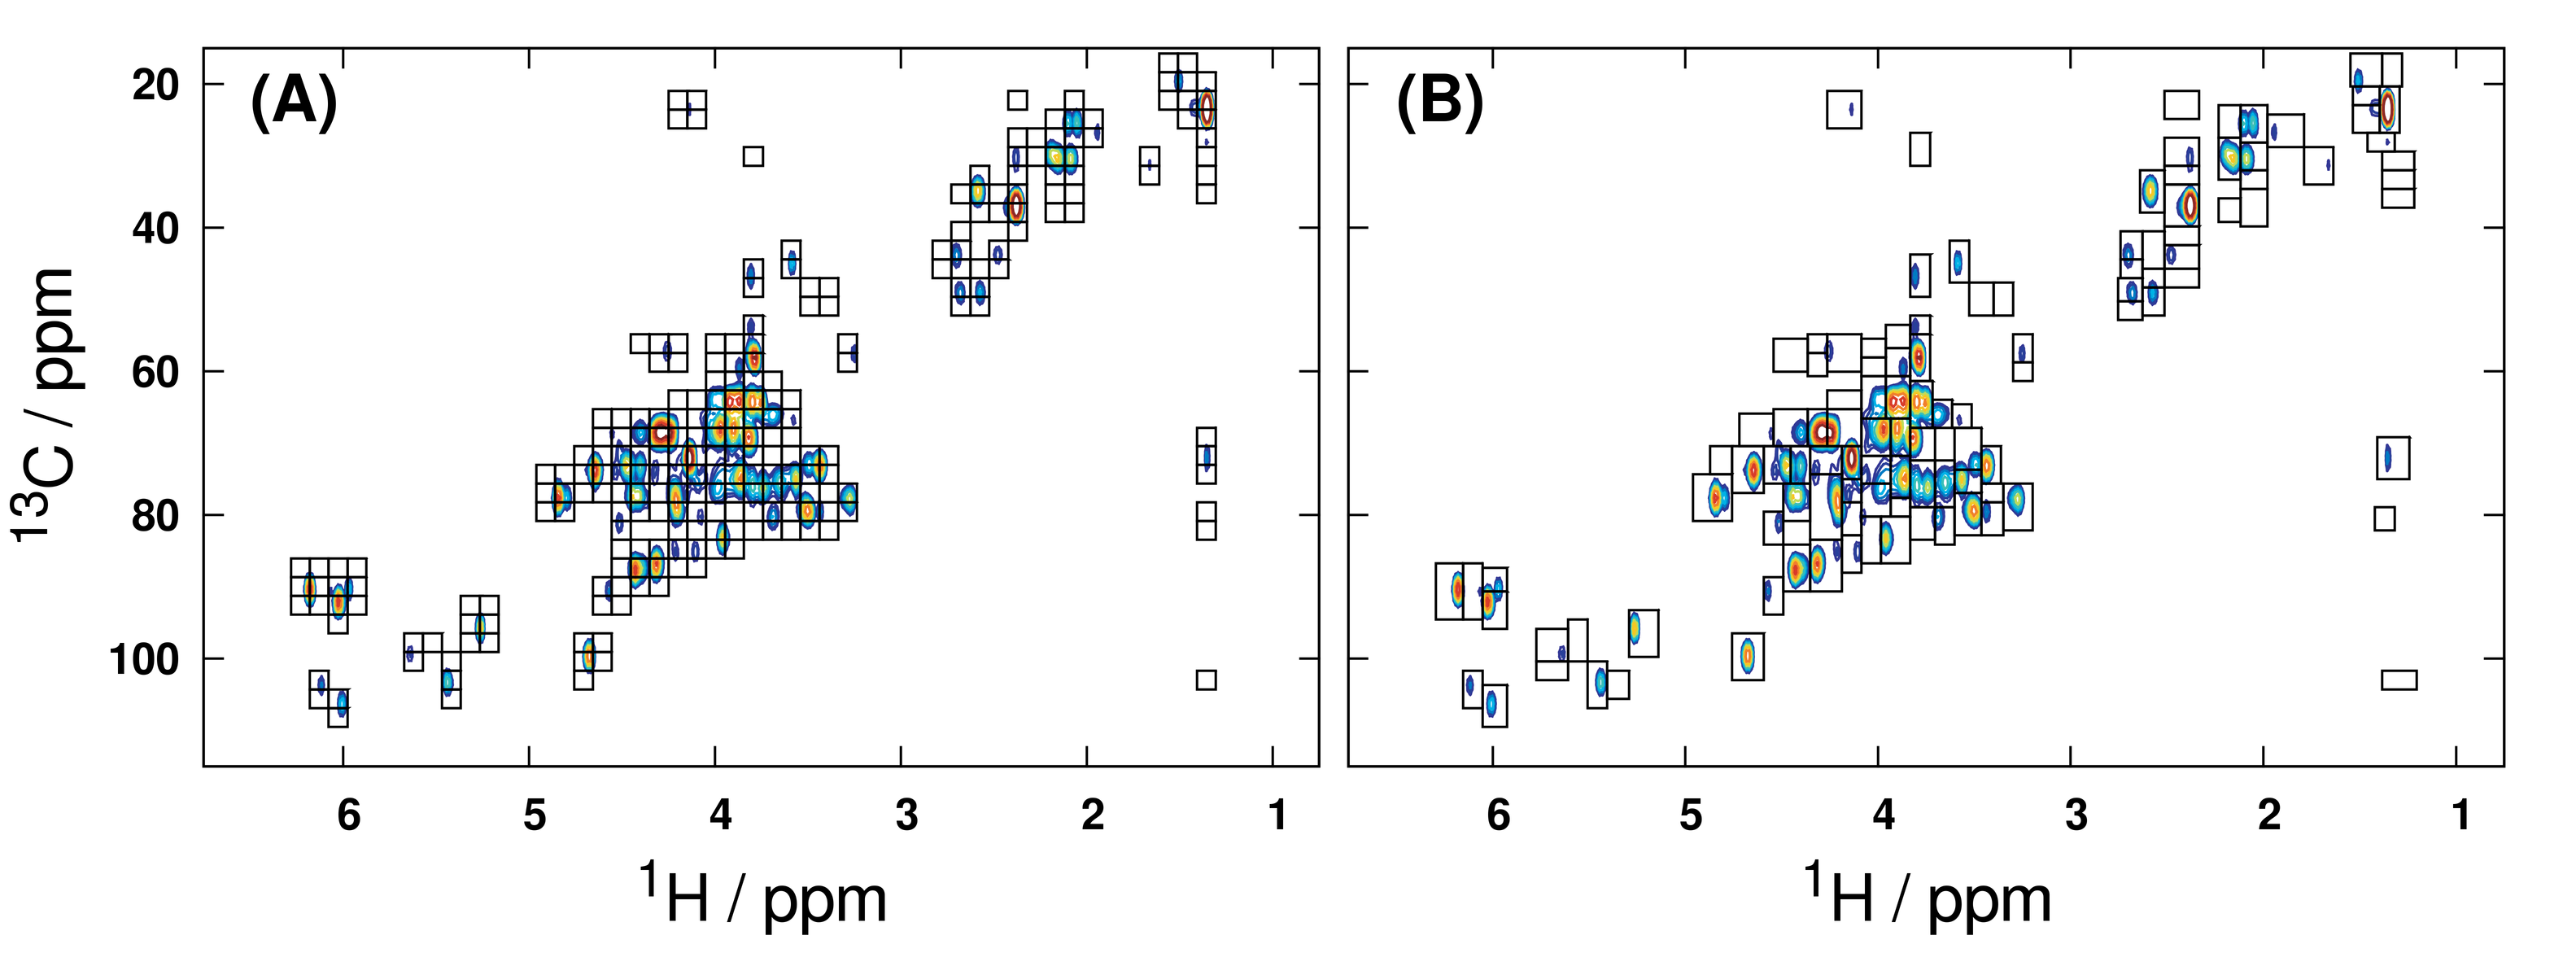
\includegraphics[width=6.5in]{figs/gaibin/02.png}
\caption
      [Binned Liver Dataset.]{
  {\bf Binned Liver Dataset.}
  \\
  Processed \hcnmr{} HSQC mean spectrum of the liver data tensor, with
  overlaid uniform ({\bf A}) and GAI ({\bf B}) bin boundaries.
}
\end{figure}

\subsection{Mouse Embryonic Fibroblast Dataset}

\begin{doublespace}
A second set of samples from kinase suppressor of Ras 1 (KSR1) knockout mouse
embryonic fibroblast (MEF) cells was also provided to generate a test
\hcnmr{} HSQC dataset for GAI-binning. For this second dataset, ten cell
samples from $ksr^{-/-}$ MEFs and ten samples from KSR1-rescued $ksr^{-/-}$
MEFs were used to produce metabolite extracts. The cells were washed, extracted
into 80:20 methanol:water, spun in a rotary evaporator, lyophilized and
redissolved according to the procedures used to extract metabolites from the
liver cell samples.
\\\\
Experiments were collected on a Bruker Avance DRX 500 MHz spectrometer equipped
with a 5 mm inverse triple-resonance (\hnmr{}, \cnmr{}, \nnmr{}) cryoprobe with
a {\it z}-axis gradient. A Bruker BACS-120 sample changer and ICON-NMR software
were used to automate data collection. A 2D gradient-enhanced \hcnmr{}
HSQC ({\it hsqcetgp}) was collected for each sample. Spectra were collected
with 128 scans and 16 dummy scans over a uniform grid of 1024 and 32 complex
points along the \hnmr{} and \cnmr{} dimensions, respectively. Spectral windows
were set to 2,359 $\pm$ 2,367 Hz along \hnmr{} and 8,174 $\pm$ 8,803 Hz along
\cnmr{}. All spectra were collected at a sample temperature of 293 K.
\end{doublespace}

\begin{figure}[ht!]
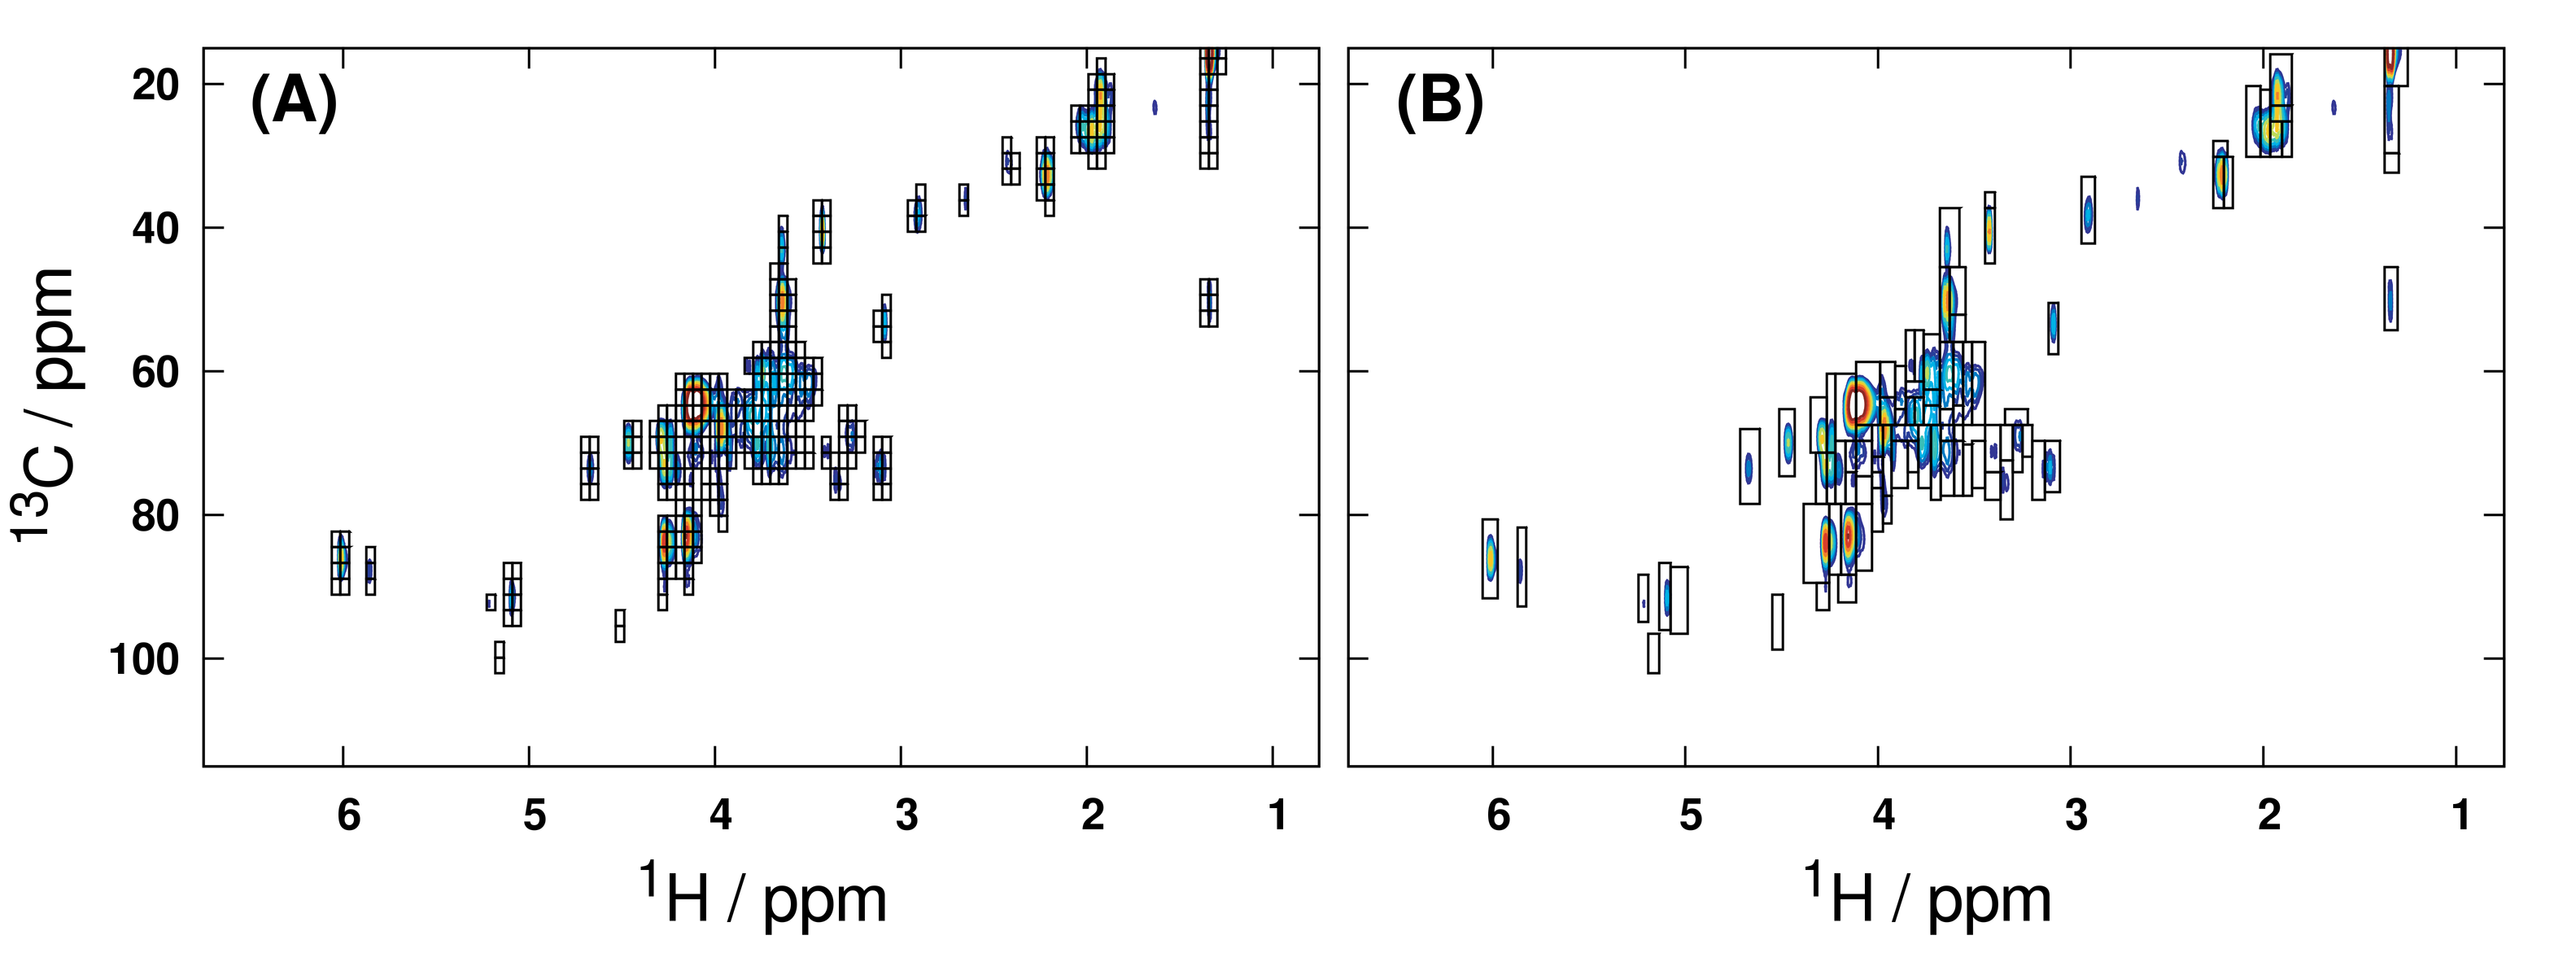
\includegraphics[width=6.5in]{figs/gaibin/03.png}
\caption
      [Binned Fibroblast Dataset.]{
  {\bf Binned Fibroblast Dataset.}
  \\
  Processed \hcnmr{} HSQC mean spectrum of the MEF data tensor, with
  overlaid uniform ({\bf A}) and GAI ({\bf B}) bin boundaries.
}
\end{figure}

\subsection{NMR Processing and Multivariate Analysis}

\begin{doublespace}
All processing, treatment and statistical modeling was performed in GNU Octave
3.6 \cite{eaton2008} using routines currently available in the MVAPACK
toolbox for NMR chemometrics \cite{worley:acscb2014}, discussed in
\hyperlink{chapter.4}{Chapter 4}. The 2D raw serial files were loaded
\cite{delaglio:jbnmr1995}, apodized with a squared-sine window,
zero-filled once along \hnmr{} and twice along \cnmr{}, and
Fourier-transformed. Spectra from the liver cell extracts were manuall
phase-corrected and cropped (1.0 -- 6.6 ppm along \hnmr{}; 16 -- 112 ppm
along \cnmr{}), and spectra from the MEF extracts were similarly phase
corrected and cropped (1.25 -- 6.2 ppm along \hnmr{}; 8 -- 102 ppm
along \cnmr{}). Both uniform and GAI-binning were performed on each data tensor
using minimum \hnmr{} and \cnmr{} bin widths of 0.025 and 2.5
ppm, respectively, and a GAI resolution parameter of 0.1. Binned regions
identified to be less intense than three times the standard deviation of the
spectral noise ($k = 3$) were removed after binning. The mean spectra of the
entire processed liver and MEF datasets, superimposed with bins identified by
both uniform and GAI-binning, are shown in Figure 6.2 and Figure 6.3.
\\\\
The applicability of GAI-binning to bilinear factorizations was demonstrated
by modeling the data tensors using both PCA and OPLS-DA. For PCA modeling of
the data, the spectral regions identified by each binning method were doubly
integrated. Scores and loadings were then calculated using the Nonlinear
Iterative Partial Least Squares (NIPALS) algorithm
\cite{jolliffe2002}. Internal leave-one-out cross-validation (LOOCV)
of each computed PCA model was performed to yield model fit (\rsqx{}) and
predictive ability (\qsq{}) statistics
\cite{krzanowski:biom1987,eshghi:cils2014}. For OPLS-DA, spectral data
points within the identified bins were vectorized row-wise into a data matrix
as previously described \cite{hedenstrom:cils2008}. During
vectorization, all data points within each binned region are stacked into an
observation vector, and data points not within bins are excluded. The use of
vectorization prior to supervised modeling facilitates the creation of
backscaled pseudospectral OPLS loadings, which hold greater ease of
interpretation over binned loadings \cite{wiklund:anchem2008}.
Modeling by an OSC-filtered NIPALS algorithm
\cite{trygg:jchemo2002} and 100 rounds of seven-fold Monte Carlo
cross-validation (MCCV) \cite{xu:jchemo2004} were performed to
compute data fit (\rsqx{}), response fit (\rsqy{}) and model predictive ability
(\qsq{}) statistics. The binned data matrices produced via double integration
were also subjected to OPLS-DA modeling in the same manner as the vectorized
data. All OPLS-DA models were further validated using CV-ANOVA
\cite{eriksson:jchemo2008} and 1,000 iterations of response
permutation testing \cite{westerhuis:metab2008} to rigorously ensure
model reliability. Backscaled predictive OPLS loadings were computed from the
vectorized bins according to previously published works
\cite{cloarec:anchem2005a,hedenstrom:cils2008}. During backscaling,
OPLS loading vectors were scaled by the inverse of their original Pareto
scaling coefficients and then unstacked into a two-dimensional pseudospectrum
using bin information. Data points not included in the vectorized loadings were
set to zero in the backscaled pseudospectrum. All data matrices were normalized
using Probabilistic Quotients (PQ) \cite{dieterle:anchem2006} and then
Pareto scaled \cite{vandenberg:bmcg2006} prior to modeling.
\end{doublespace}

\section{Results and Discussion}

\begin{doublespace}
Processing of the liver extract spectra yielded a real data tensor of 24
\hcnmr{} HSQC spectra having 442$\times$149 points each, and processing of the
fibroblast spectra yielded a tensor of 17 spectra having 1,071$\times$172
real data points each. The observation counts ($N$), variable counts ($K$)
and PCA/OPLS cross-validation statistics (\rsq{}, \qsq{}) for each dataset and
variable reduction method are summarized in Table 6.1. Further validation
results from the OPLS models, all of which indicate varying degrees of high
model reliability, are also summarized in Table 6.2. Through examination of the
variable counts within Table 6.1, it is readily apparent that GAI-binning is
dramatically more effective than uniform binning at discriminating between
signal and noise regions within spectral data. On average, GAI-binning
segmented each data tensor into less than half the number of bins produced by
uniform binning, and produced PCA models with markedly higher \rsqx{} and
\qsq{} statistics. Moreover, even with the greatly reduced variable counts
produced by GAI-binning relative to uniform binning, the OPLS \qsq{} statistics
between the two methods are statistically indistinguishable. In fact, the
variable counts resulting from GAI-binning these third-order tensors are
substantially lower than the few hundred variables typically produced by
binning {\it one}-dimensional spectra. Resulting scores from PCA modeling
of the GAI-binned liver data tensor are shown in Figure 6.4.
\end{doublespace}

\begin{table}[h!]
\caption{Data Matrices and PCA/OPLS Model Statistics.}
\begin{center}
\begin{tabular}{l l | l l l l l | l l l}
  \hline
              &         &
    \multicolumn{5}{c|}{{\bf Integration}} &
    \multicolumn{3}{c}{{\bf Vectorization}} \\
              &         &
    \multicolumn{3}{c}{PCA} &
    \multicolumn{2}{c|}{OPLS} & &
    \multicolumn{2}{c}{OPLS} \\
  \hline
              &         &
    $K$       & \rsqx{} & \qsq{} & \rsqy{} & \qsq{} &
    $K$                          & \rsqy{} & \qsq{} \\
  \hline
  {\bf Liver} & Unif.   &
    248       & 0.82    & 0.71   & 0.993   & 0.938 $\pm$ 0.002 &
    11,160                       & 0.993   & 0.929 $\pm$ 0.003 \\
  $N = 24$    & GAI     &
    113       & 0.89    & 0.75   & 0.991   & 0.928 $\pm$ 0.003 &
    10,474                       & 0.994   & 0.933 $\pm$ 0.003 \\
  \hline
  {\bf MEF}   & Unif.   &
    334       & 0.48    & 0.40   & 0.994   & 0.974 $\pm$ 0.004 &
    18,348                       & 0.994   & 0.963 $\pm$ 0.005 \\
  $N = 17$    & GAI     &
    93        & 0.71    & 0.56   & 0.994   & 0.973 $\pm$ 0.005 &
    18,789                       & 0.996   & 0.962 $\pm$ 0.006
\end{tabular}
\end{center}
\end{table}

\begin{table}[h!]
\caption{OPLS-DA Cross Validation $p$-values.}
\begin{center}
\begin{tabular}{l l | l l | l l}
  \hline
              &       &
    \multicolumn{2}{c|}{{\bf Integration}} &
    \multicolumn{2}{c}{{\bf Vectorization}} \\
              &       & Permutation & CV-ANOVA & Permutation & CV-ANOVA \\
  \hline
  {\bf Liver} & Unif. &
    $< 0.001$ & $3.24 \times 10^{-11}$ & $< 0.001$ & $4.70 \times 10^{-11}$ \\
  $N = 24$    & GAI   &
    $< 0.001$ & $3.34 \times 10^{-10}$ & $< 0.001$ & $9.74 \times 10^{-11}$ \\
  \hline
  {\bf MEF}   & Unif. &
    $< 0.001$ & $3.56 \times 10^{-10}$ & $< 0.001$ & $1.73 \times 10^{-9}$ \\
  $N = 24$    & GAI   &
    $< 0.001$ & $1.37 \times 10^{-9}$  & $< 0.001$ & $2.34 \times 10^{-9}$
\end{tabular}
\end{center}
\end{table}

\begin{SCfigure}
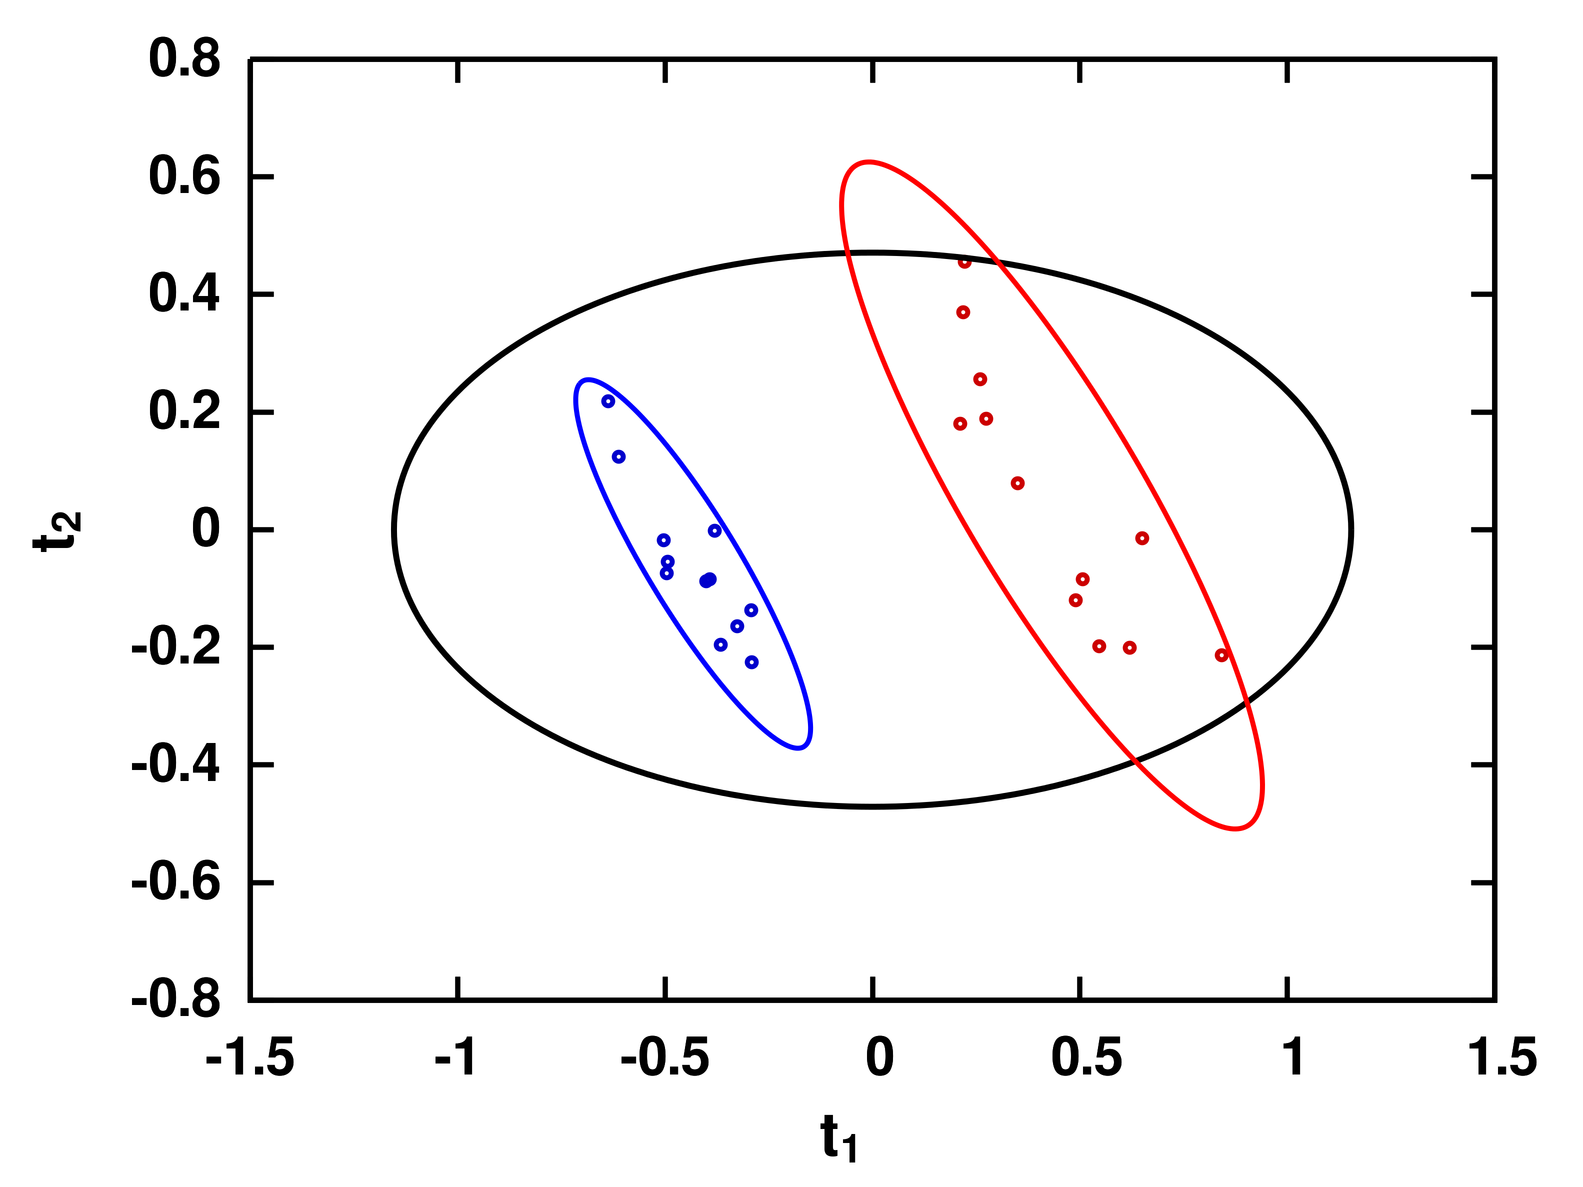
\includegraphics[width=3.5in]{figs/gaibin/04.png}
\caption
      [PCA Scores of a GAI-binned Tensor.]{
  {\bf PCA Scores of a GAI-binned Tensor.}
  \\
  Principal component analysis scores resulting from modeling the GAI-binned
  \hcnmr{} HSQC liver data matrix, indicating a high degree of separation
  between experimental groups. Model \rsqx{} and \qsq{} were 0.68 and 0.64 for
  the first principal component ($t_1$) and 0.12 and 0.09 for the second
  ($t_2$). Class separations of this magnitude are readily achievable using
  data matrices generated by GAI-binning, due in large part to the low variable
  counts it generally produces.
}
\end{SCfigure}

\begin{doublespace}
Backscaled predictive OPLS-DA loadings of the vectorized \hcnmr{} HSQC spectral
data tensors (Figure 6.5) lend further support for the use of multidimensional
binning in metabolic fingerprinting studies. Even when vectorization is
performed in place of integration to produce a data matrix, binning offers an
effective means of variable selection: only 10,474 of 65,858 variables (16\%)
were retained when GAI-binning was used as a pre-filter prior to modeling the
liver data. A similar reduction was observed in the fibroblast dataset, where
GAI-binning retained 18,789 of 184,212 total variables for a 90\% reduction in
dimensionality. These substantially reduced variable counts offered by binning
translate to more well-conditioned bilinear modeling problems. As the
dimensionality of the input dataset is increased further, the reductions in
variable count afforded by multidimensional binning are expected to become even
more dramatic. While the variable counts produced by vectorization of uniformly
binned data tensors are comparable to those from GAI-binning, it is critical to
recognize that the uniformly binned regions contain more noise data points than
their GAI-binned counterparts, and thus offer a less efficient dimensionality
reduction.
\\\\
Spectral regions produced by GAI-binning (Figure 6.2) demonstrate several
important properties of the combined binning and noise removal processes.
Because $t_1$ noise and truncation artifacts yield phase-incoherent negative
spectral excursions after Fourier transformation, `unrelaxed' GAI-binning
($R = 1$) tends to preferentially subdivide near such regions, producing
elongated bins along the $F_1$ dimension. Decreasing the resolution parameter
from its maximum value shrinks these bins to contain only true signals. Thus,
an objective rule for determining an optimal resolution parameter during
binning is to decrease $R$ until all bins shrink to contain a minimal amount
of noise. Once an optimal resolution parameter has been identified, a suitable
noise threshold ($k$) must be determined such that all noise bins are removed
without loss of bins containing weak signals. However, once $R$ and $k$ have
been determined for a given set of experimental conditions, they may be applied
during GAI-binning to any data collected at later times under the same
conditions to achieve ideal results. The selections of resolution parameter
($R = 0.1$) and noise threshold ($k = 3$) made in this work were identified
according to the above criteria through a manual visual examination of the
binning results, but it is conceivable that objective metrics of these criteria
could be constructed that facilitate automated determination of these
parameters.
\\\\
Finally, like AI-binning, the execution time of GAI-binning scales
quadratically with the number of spectral data points, and scales approximately
linearly with both the number of spectral dimensions and the number of
observations. Typical runtimes for binning two-dimensional datasets range from
seconds to a few minutes, depending mostly on the data point count. Thus,
while zero-filling may be used to increase the digital resolution of data
being input into GAI-binning, it should be applied sparingly to avoid
unnecessarily long computation times during bin region determination.
\end{doublespace}

\begin{figure}[hb!]
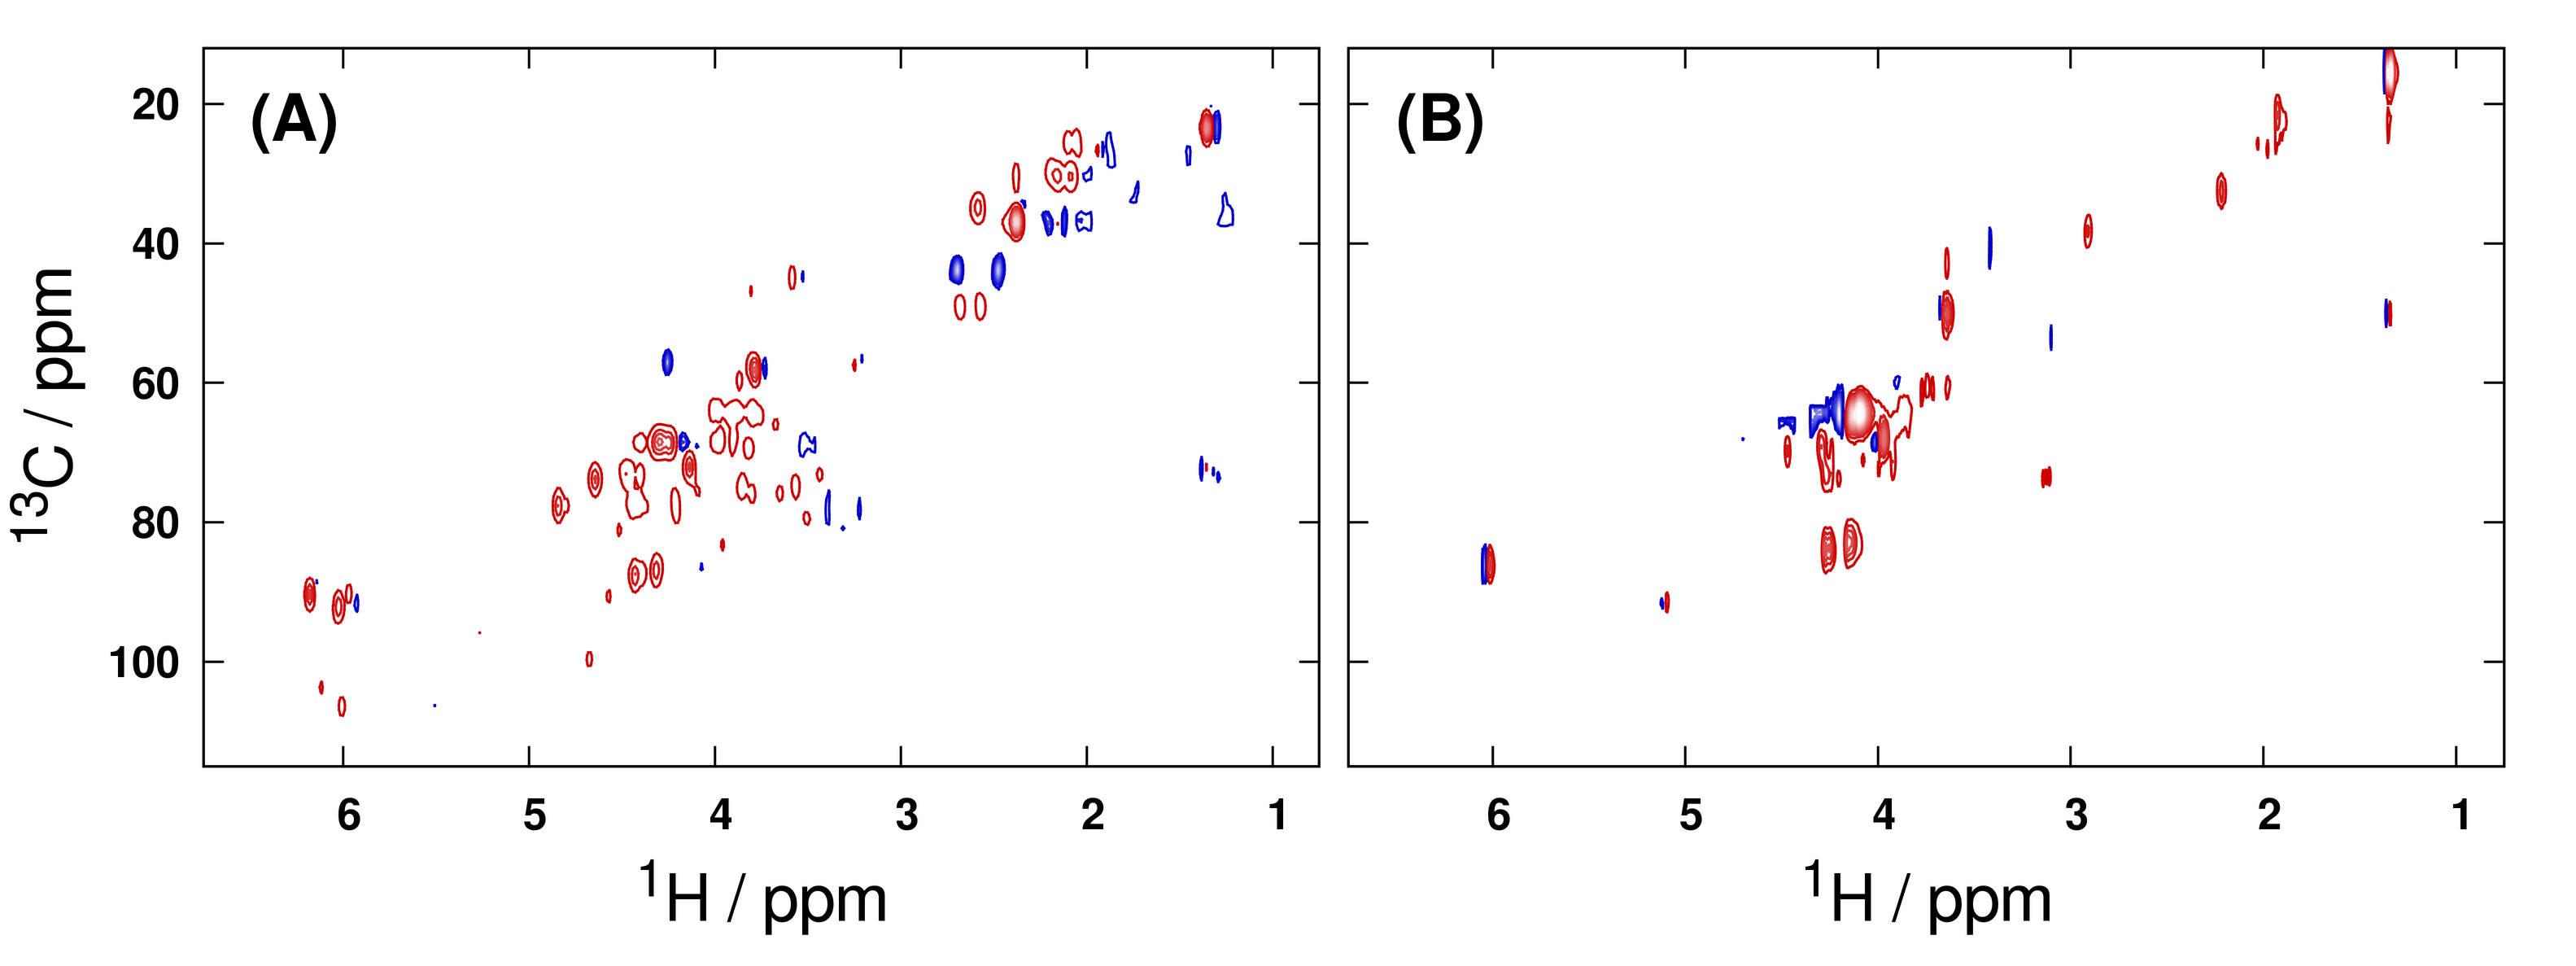
\includegraphics[width=6.5in]{figs/gaibin/05.png}
\caption
      [Pseudospectral HSQC Loadings.]{
  {\bf Pseudospectral HSQC Loadings.}
  \\
  Backscaled full-resolution pseudospectral loadings from OPLS-DA modeling of
  the GAI-reduced ({\bf A}) liver and ({\bf B}) fibroblast \hcnmr{} HSQC data
  tensors. Positive and negative loadings are represented by red and blue
  contours, respectively.
}
\end{figure}

\section{Conclusions}

\begin{doublespace}
Generalized Adaptive Intelligent binning is a logical extension of the
previously described Adaptive Intelligent binning algorithm
\cite{demeyer:anchem2008} to multidimensional datasets, and provides a
model-free alternative to peak-fitting and peak-picking as a means of variable
selection in multivariate analyses. Furthermore, GAI-binning is a more
intelligent method to extract signal regions from multidimensional spectral
data tensors than uniform binning, and may be used to generate very
low-dimensionality data matrices via multiple integration or efficiently
noise-filtered data matrices via vectorization. The C++ implementations of
1D and 2D GAI-binning used in this work are freely available as part of the
MVAPACK software package \cite{worley:acscb2014} introduced in
\hyperlink{chapter.4}{Chapter 4}.
\end{doublespace}

\section{Permutation Test Results}

\begin{figure}[ht!]
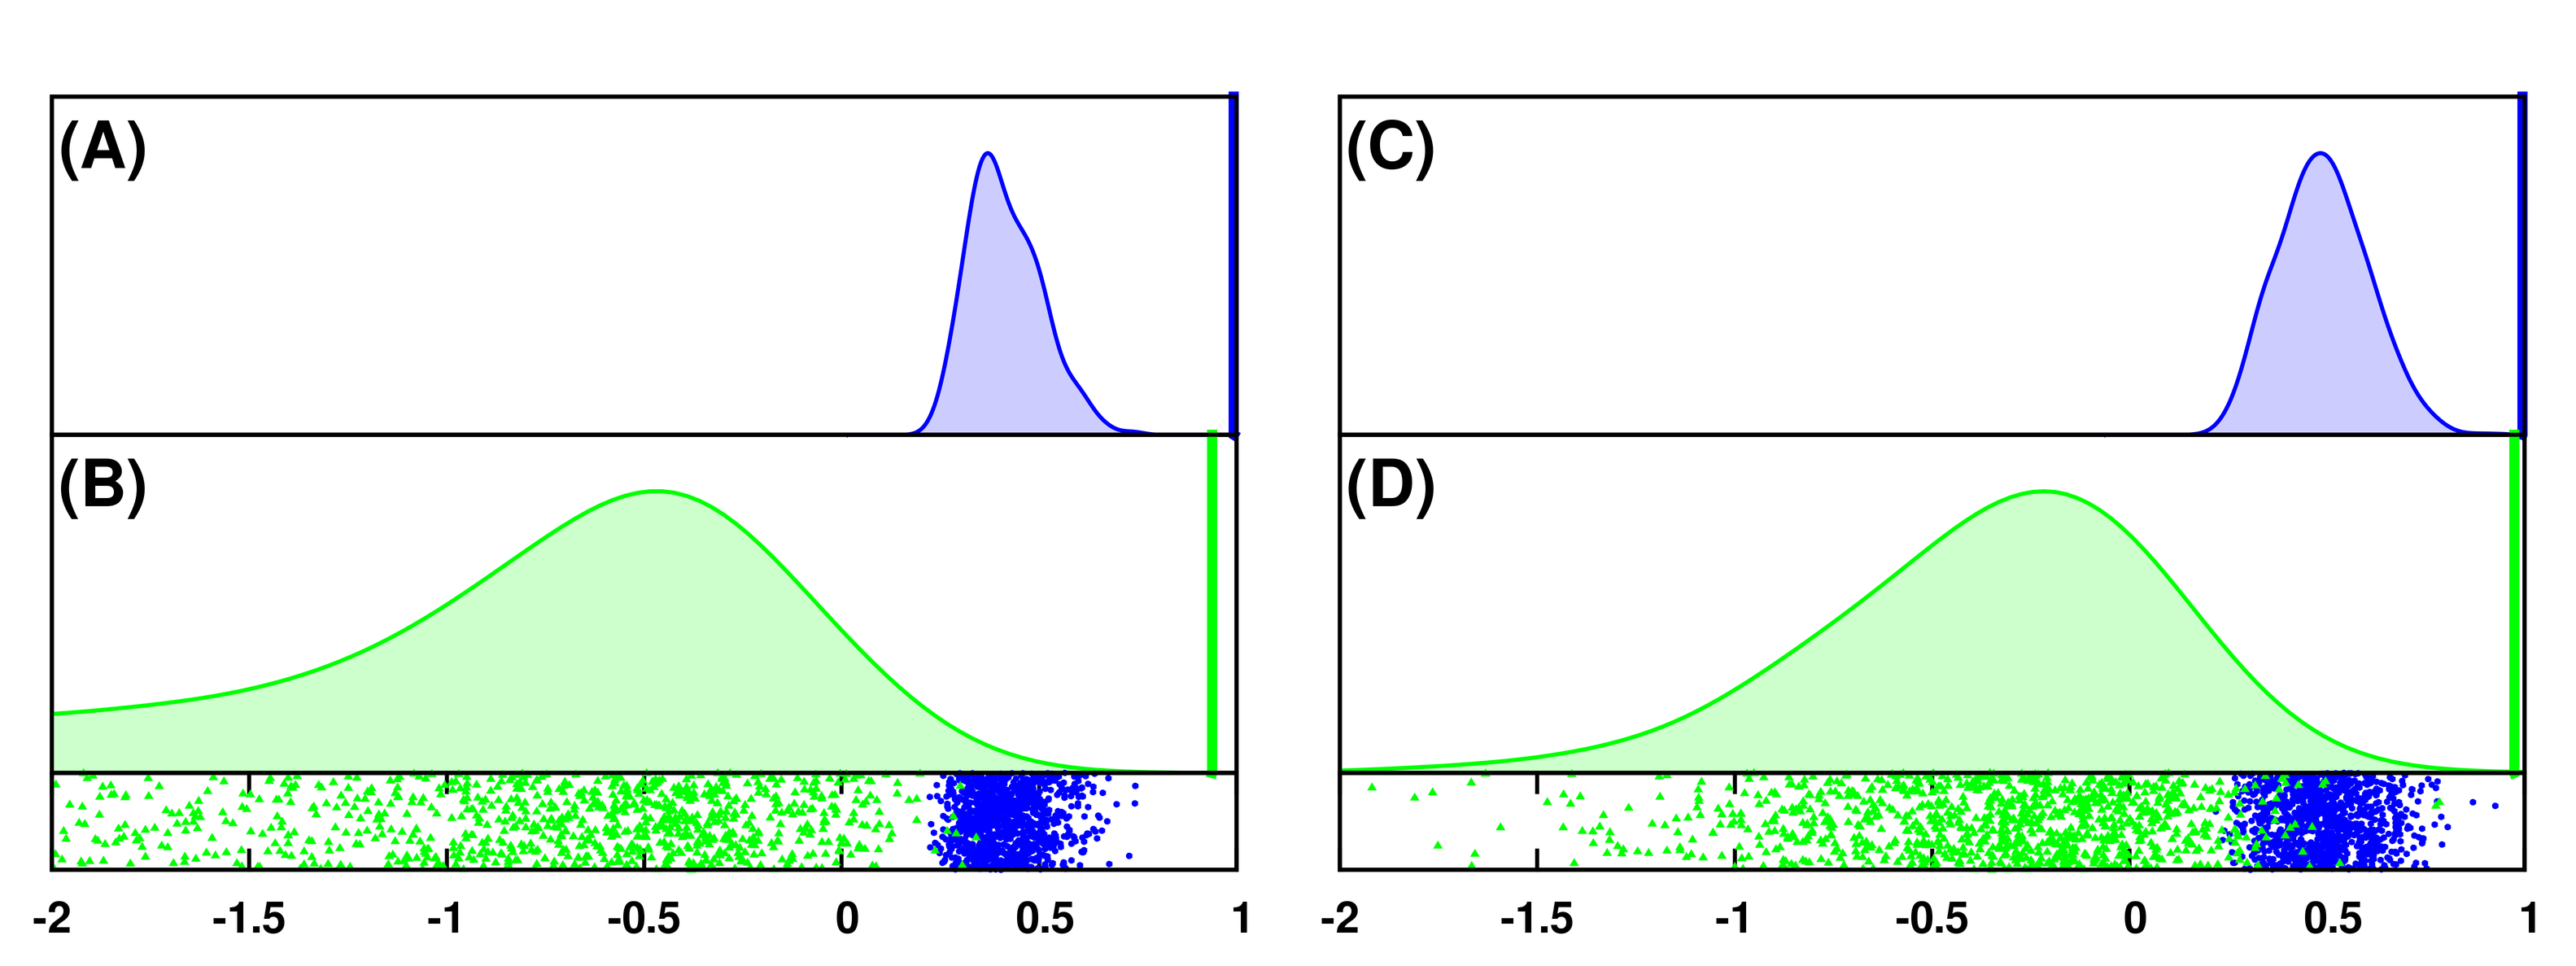
\includegraphics[width=6.5in]{figs/gaibin/06.png}
\caption
      [Response Permutation Test: Uniform integration.]{
  {\bf Response Permutation Test: Uniform integration.}
  \\
  Response permutation test results for OPLS-DA models from the uniformly
  binned (integrated) liver ({\bf A}, {\bf B}) and fibroblast
  ({\bf C}, {\bf D}) data tensors. Model fit (\rsqy{}) statistics
  ({\bf A}, {\bf C}) are shown in blue, and model predictive ability (\qsq{})
  statistics ({\bf B}, {\bf D}) are shown in green. True values of \rsqy{} and
  \qsq{} are represented by vertical bars, and null distributions are computed
  through kernel density estimation of the values from permutation. Scatter
  plots of the permutation (null) \rsqy{} and \qsq{} statistics are shown in
  the lower panes.
}
\end{figure}

\begin{figure}[ht!]
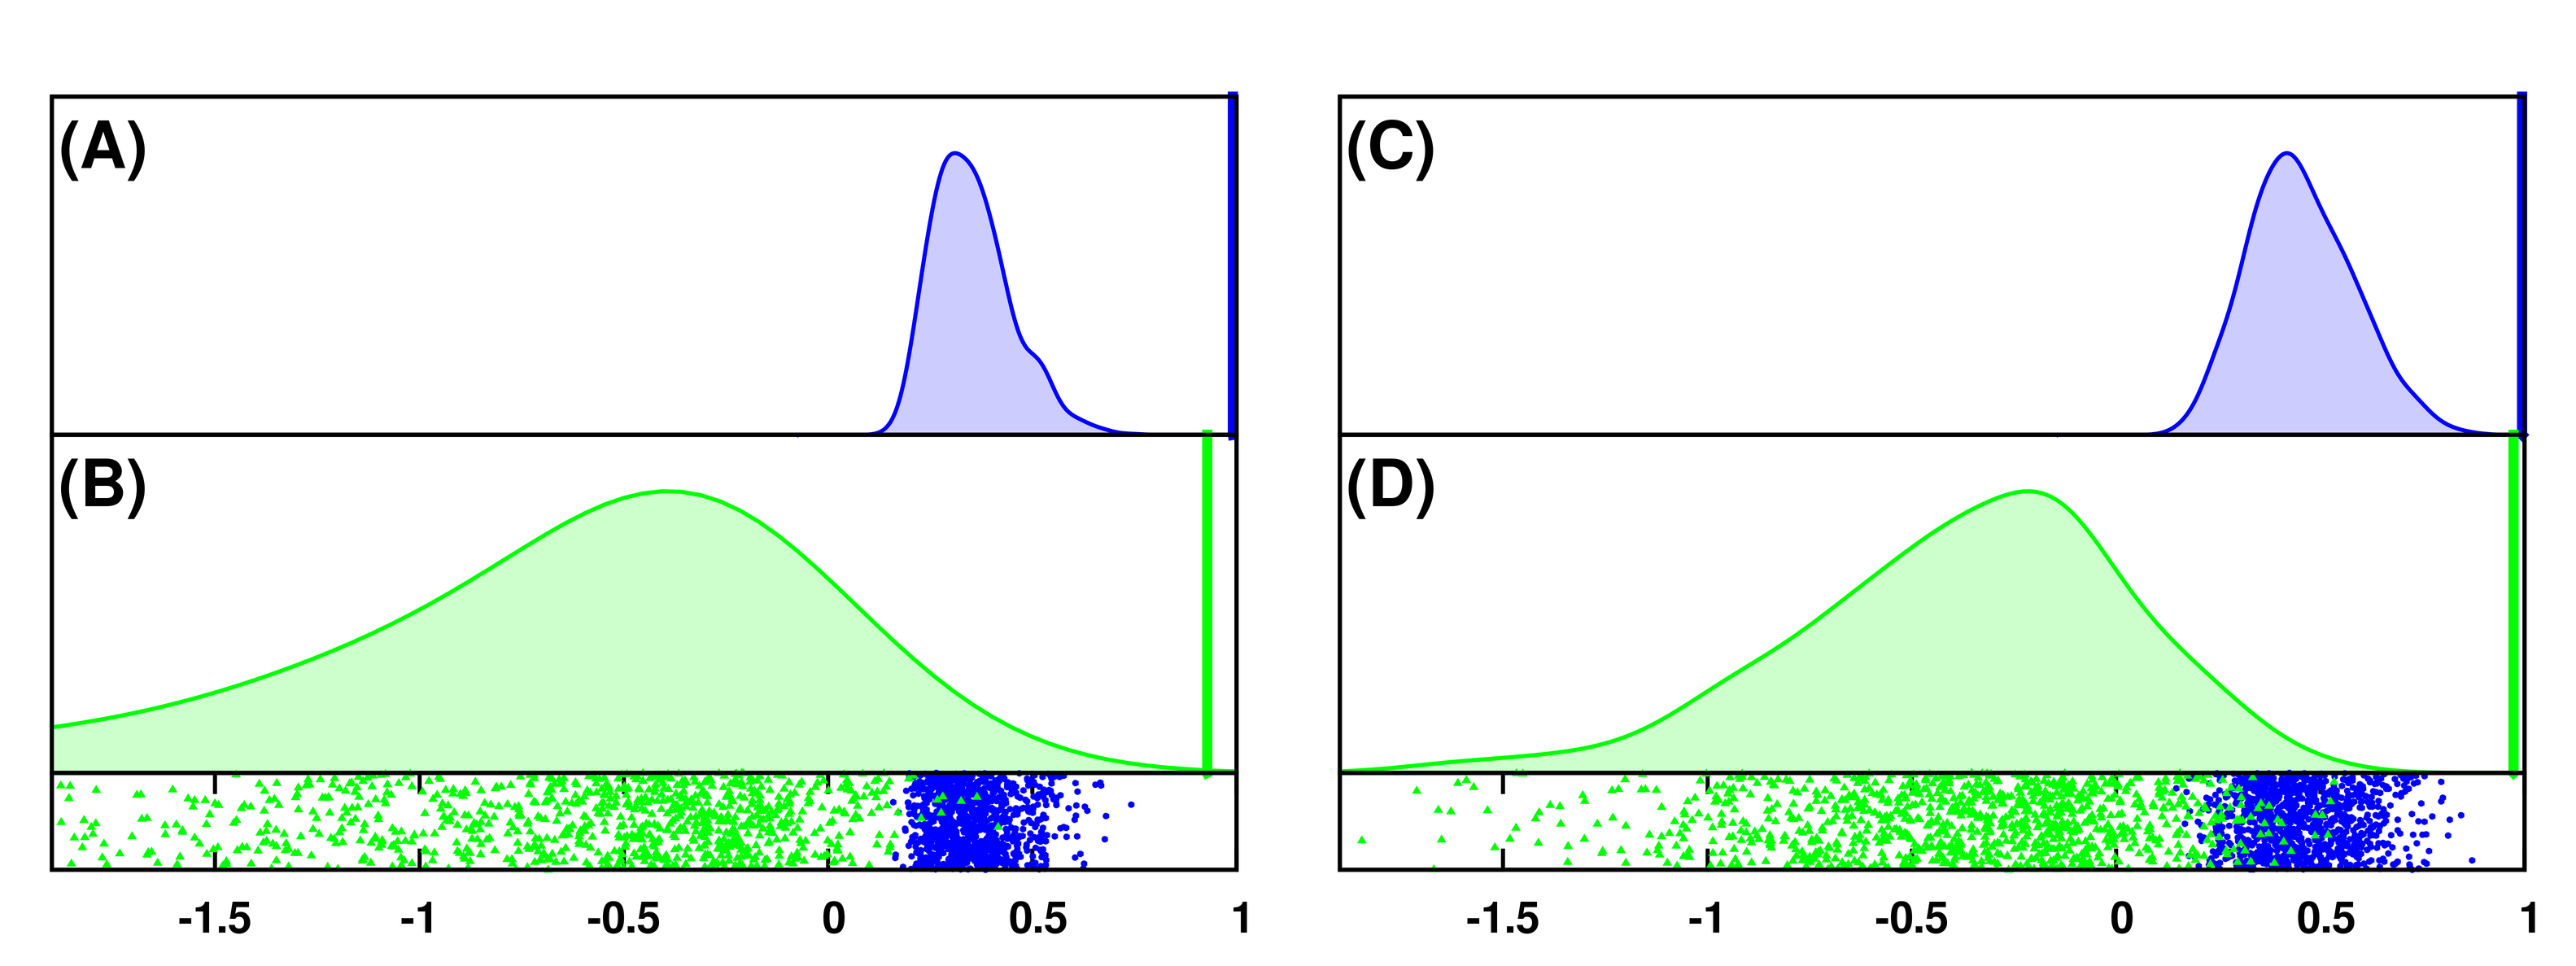
\includegraphics[width=6.5in]{figs/gaibin/07.png}
\caption
      [Response Permutation Test: GAI-integration.]{
  {\bf Response Permutation Test: GAI-integration.}
  \\
  Response permutation test results for OPLS-DA models from the GAI-binned
  (integrated) liver ({\bf A}, {\bf B}) and fibroblast
  ({\bf C}, {\bf D}) data tensors. See the caption of Figure 6.6 for a
  complete description of the figure contents.
}
\end{figure}

\begin{figure}[ht!]
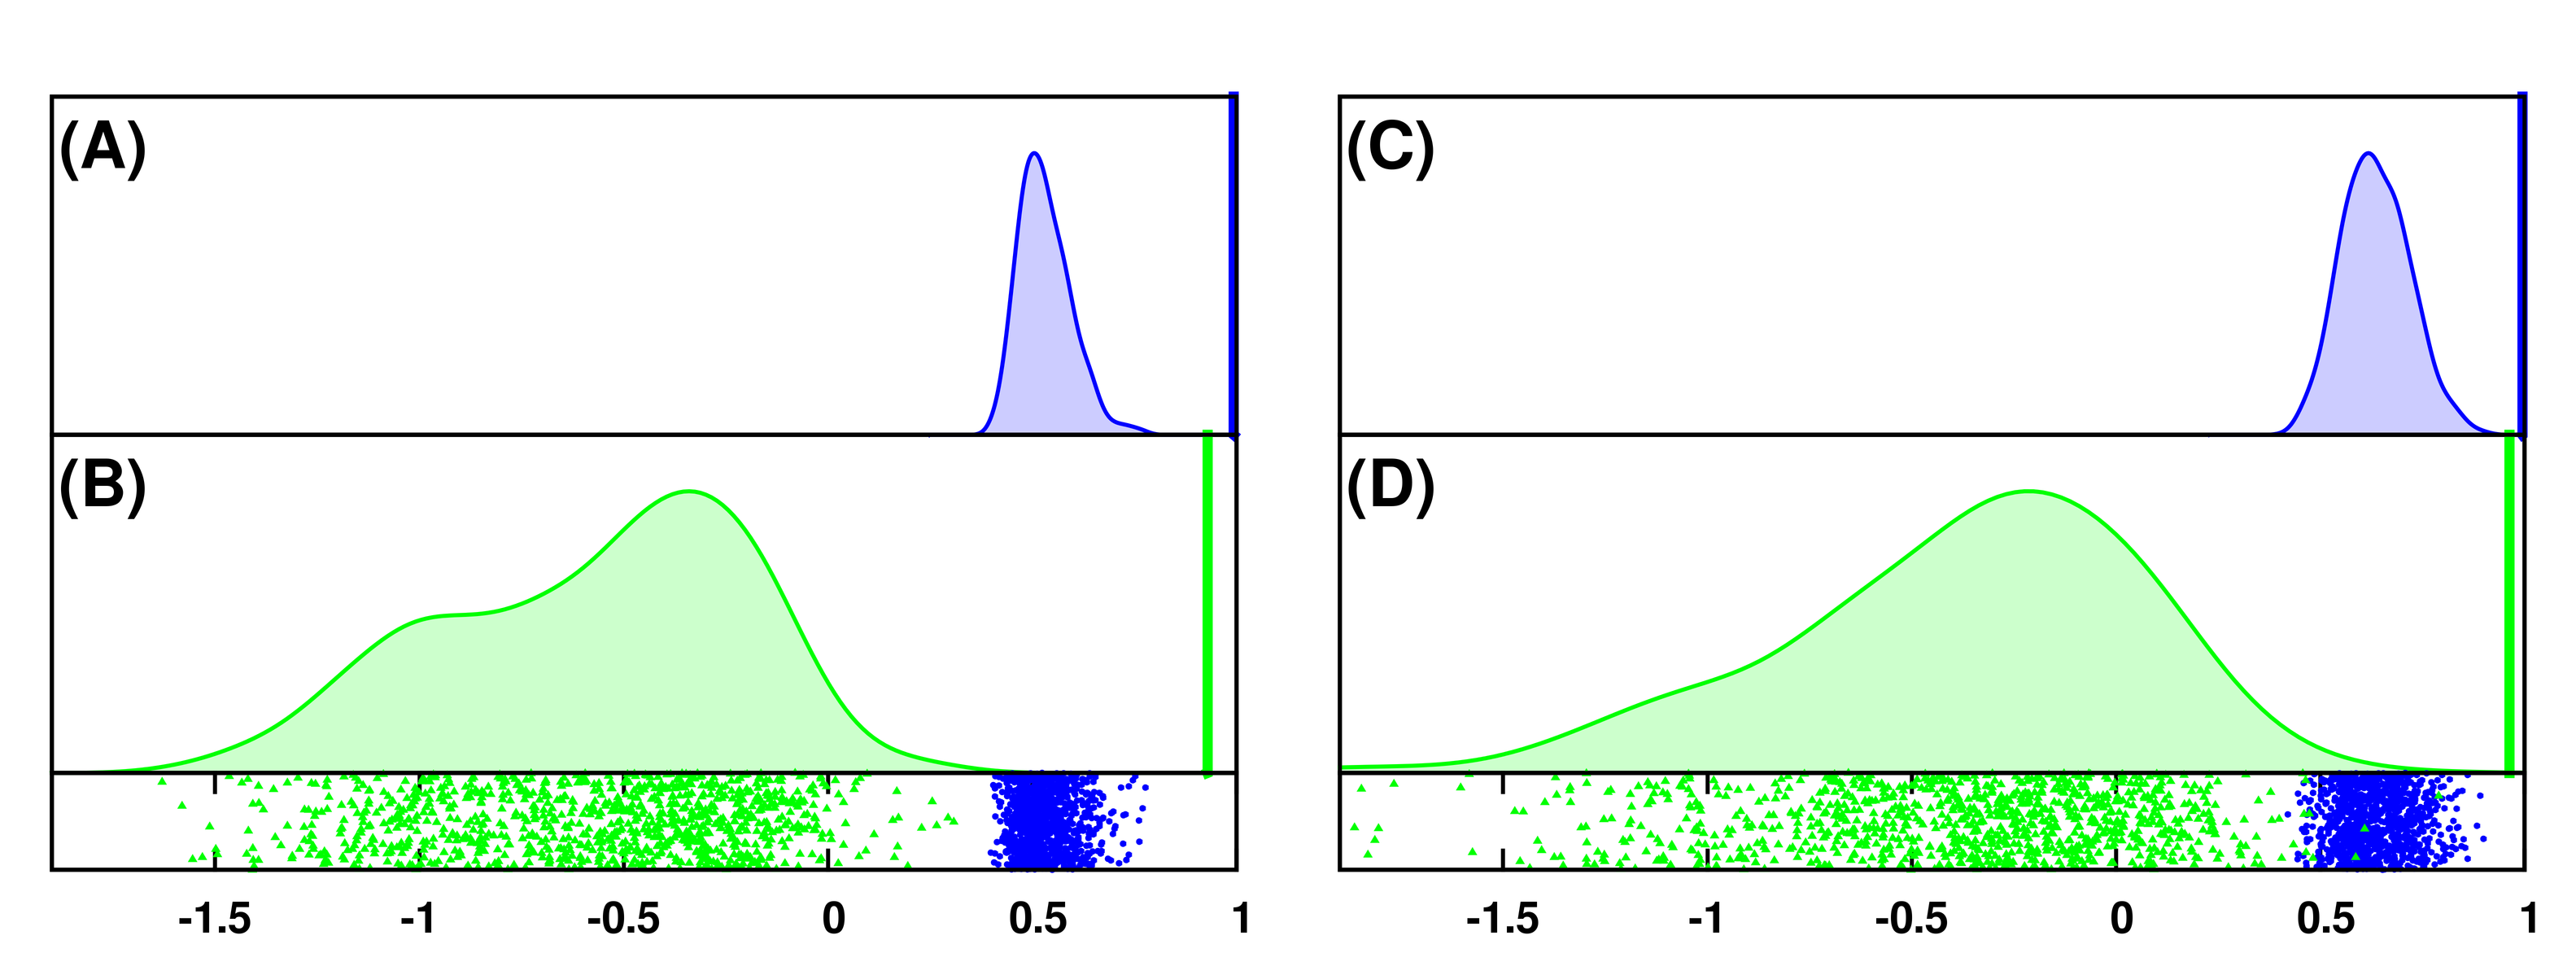
\includegraphics[width=6.5in]{figs/gaibin/08.png}
\caption
      [Response Permutation Test: Uniform vectorization.]{
  {\bf Response Permutation Test: Uniform vectorization.}
  \\
  Response permutation test results for OPLS-DA models from the uniformly
  binned (vectorized) liver ({\bf A}, {\bf B}) and fibroblast
  ({\bf C}, {\bf D}) data tensors. See the caption of Figure 6.6 for a
  complete description of the figure contents.
}
\end{figure}

\begin{figure}[ht!]
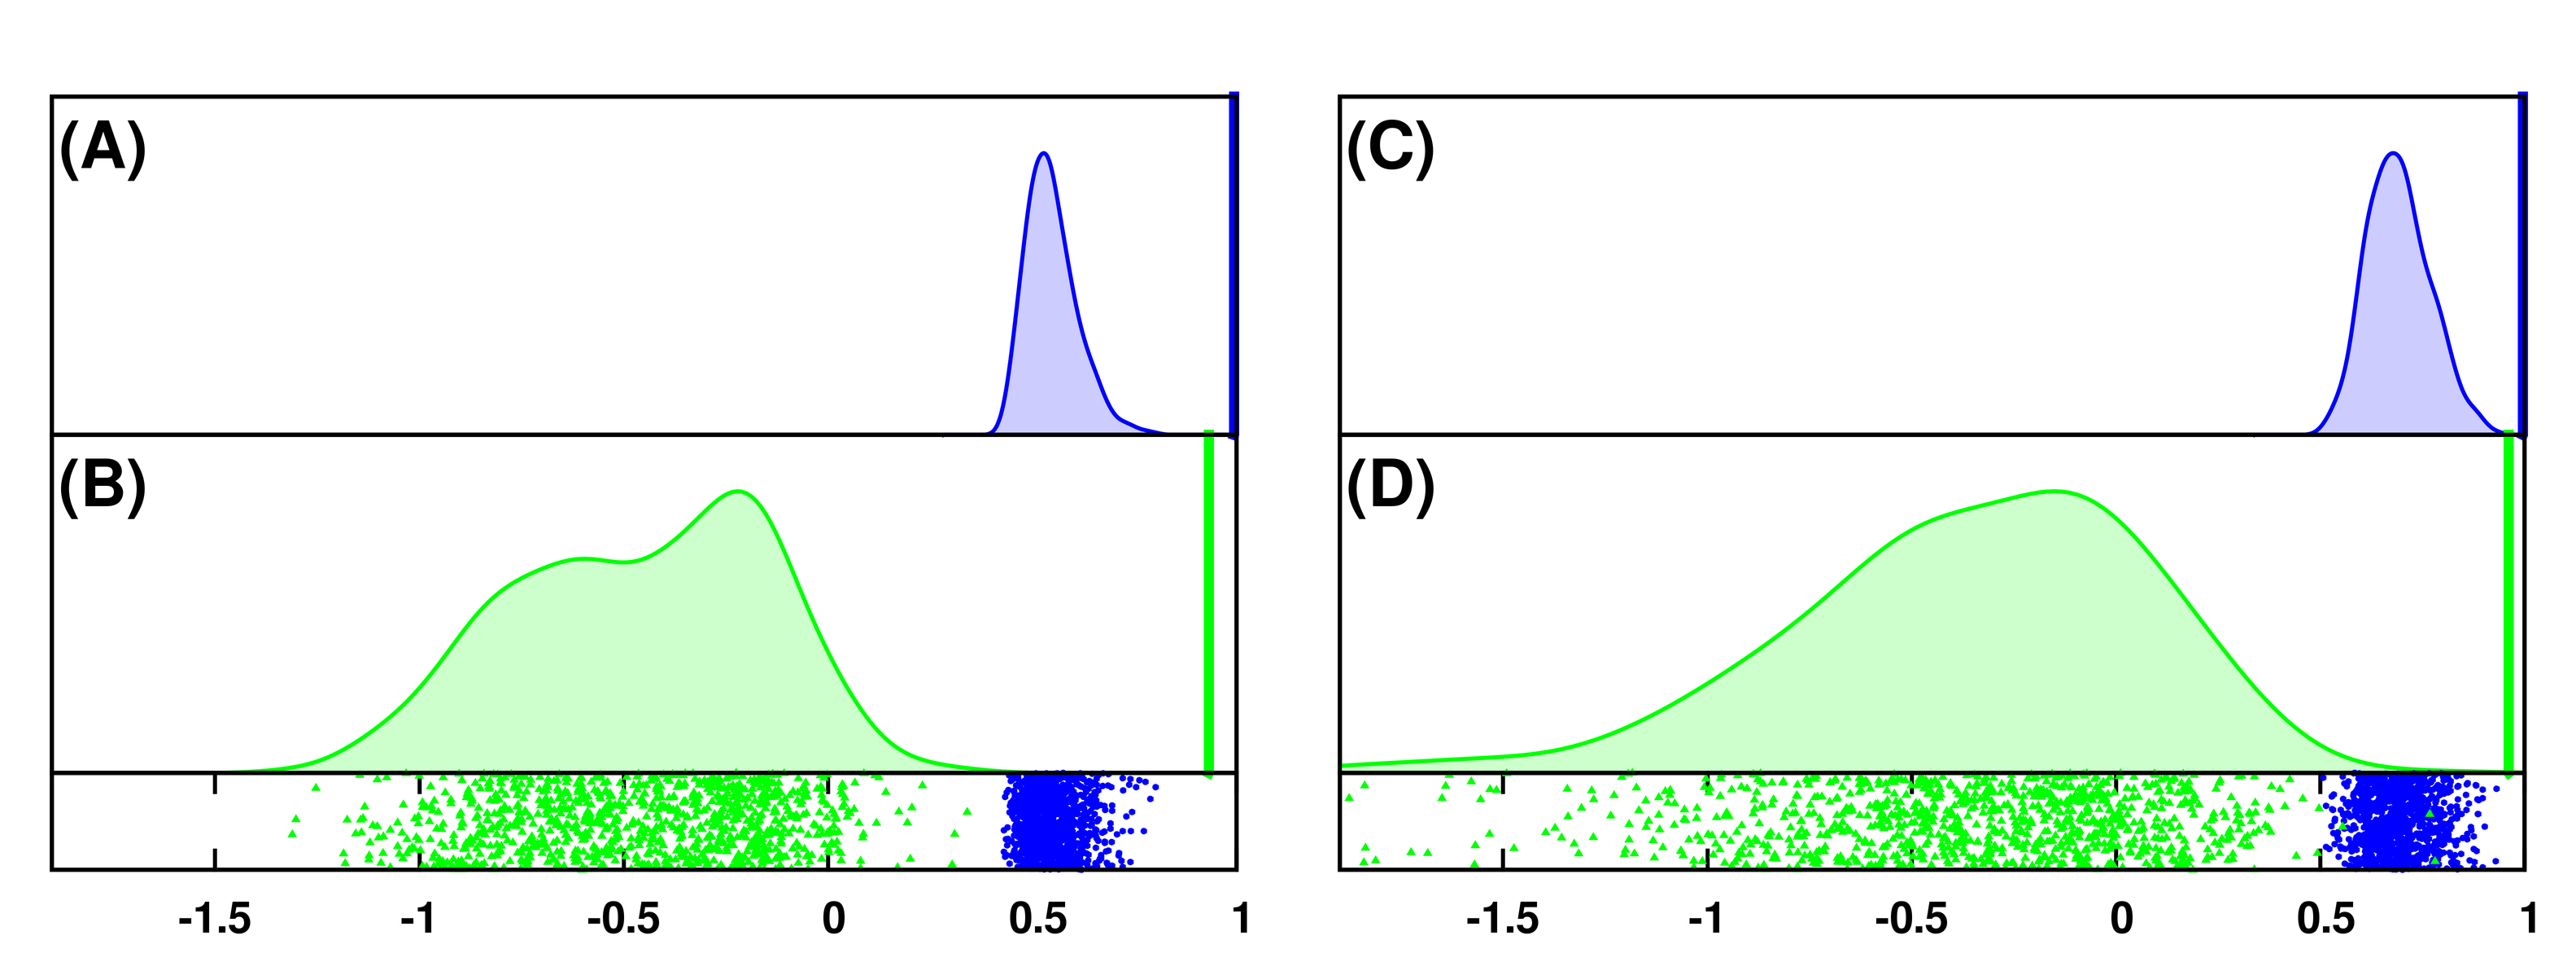
\includegraphics[width=6.5in]{figs/gaibin/09.png}
\caption
      [Response Permutation Test: GAI-vectorization.]{
  {\bf Response Permutation Test: GAI-vectorization.}
  \\
  Response permutation test results for OPLS-DA models from the GAI-binned
  (vectorized) liver ({\bf A}, {\bf B}) and fibroblast
  ({\bf C}, {\bf D}) data tensors. See the caption of Figure 6.6 for a
  complete description of the figure contents.
}
\end{figure}

\pagebreak
\bibliographystyle{abbrv}
\bibliography{bworley}



\chapter{Quantification of PCA/PLS-DA Class Separations}

\begin{quote}
{\it
  People want to see patterns in the world. ... So important is this skill
  that we apply it everywhere, warranted or not.}
\\\\
 -- Benoit Mandelbrot
\end{quote}

\section{Introduction}

\begin{doublespace}
The importance placed on interpretation of PCA, PLS-DA and OPLS-DA scores plots
necessitates the use of quantitative procedures to determine the significance
of separations between multiple experimental groups in scores space. However,
no de facto protocol or metric exists to provide a means of reporting the
degree or significance of group separation
\cite{werth:abio2010,goodpaster:abio2010,goodpaster:cils2011}.
Anderson et al. used the $J_2$ criterion
\cite{anderson:metab2008,koutroumbas2006} to assess the quality of
resulting scores clusters according to the average withing-group and
between-group scatters for all groups. However, the $J_2$ metric only provides
an overall estimate of group separation without fine-grained information on
each pair of groups \cite{koutroumbas2006}. A similar problem exists
with the related Davies-Bouldin index \cite{davies:ieee1979}, which
chooses a worst-case estimate of group overlap as its figure of merit. Dixon
et al. \cite{dixon:jchemo2009} also comprehensively reported the
performances of four cluster separation indices based on modifications of
metrics used to validate separation for unsupervised clustering algorithms.
Alternatively, the PCAtoTree protocol constructs dendrograms from Euclidean
distance matrices computed from PCA scores for the PHYLIP
\cite{felsenstein:clad1989} software suite using a bootstrapping routine to
determine branch node significance \cite{werth:abio2010,retief:mmbio2000}.
However, it was recently shown that hypothesis testing using a Mahalanobis
distance metric and the $T^2$ and $F$ distributions can provide a statistical
means of quantifying group similarity \cite{goodpaster:cils2011}, suggesting
the possibility of returning $p$ values for full statistical quantitation of
group separations in scores space.
\end{doublespace}

\section{Materials and Methods}

\begin{doublespace}
The methods described below were implemented in software using the C
programming language with minimal external dependencies, so the programs
may be compiled and executed on any modern GNU/Linux distribution.
\end{doublespace}

\subsection{Probability Calculation}

\begin{doublespace}
Under the assumption that each group in the scores space is distributed as a
multivariate normal random variable, the separations between groups may be
calculated using the squared Mahalanobis distance metric
\cite{mahalanobis:pnisi1936}:

\begin{equation}
D_M^2 =
  (\mathbf{u}_j - \mathbf{u}_i)^T
  \mathbf{S}_p^{-1}
  (\mathbf{u}_j - \mathbf{u}_i)
\end{equation}

In the above equation, $\mathbf{u}_i, \mathbf{u}_j \in \mathbb{R}^p$ are the
$p$-variate sample means of groups $i$ and $j$, respectively, and
$\mathbf{S}_p \in \mathbb{R}^{p \times p}$ is the pooled variance-covariance
matrix, a weighted sum of the covariance matrices from groups $i$ and
$j$:

\begin{equation}
\mathbf{S}_p = \frac{n_i \mathbf{S}_i + n_j \mathbf{S}_j}{n_i + n_j}
\end{equation}

where $n_i$ and $n_j$ are the number of observations in groups $i$ and $j$,
respectively. The Mahalanobis distance may then be related to a Hotelling's
$T^2$ statistic by the following scaling \cite{mardia1979}:

\begin{equation}
T^2 = \left( \frac{n_i n_j}{n_i + n_j} \right) D_M^2
\end{equation}

This $T^2$ statistic is an extension of the Student's $t$ statistic to
hypothesis tests in multiple dimensions, and may be related to an $F$
distribution by a final scaling \cite{mardia1979}:

\begin{equation}
x_F =
  \frac{n_i + n_j - p - 1}{p (n_i + n_j - 2)} T^2 \sim
  F(p, n_i + n_j - p - 1)
\end{equation}

It can be seen from this final relation that evaluation of the complement of
the cumulative $F$-distribution function at $x_F$ yields the $p$ value for
accepting the null hypothesis: the points in groups $i$ and $j$ are in fact
drawn from the same distribution.
\end{doublespace}

\begin{figure}[ht!]
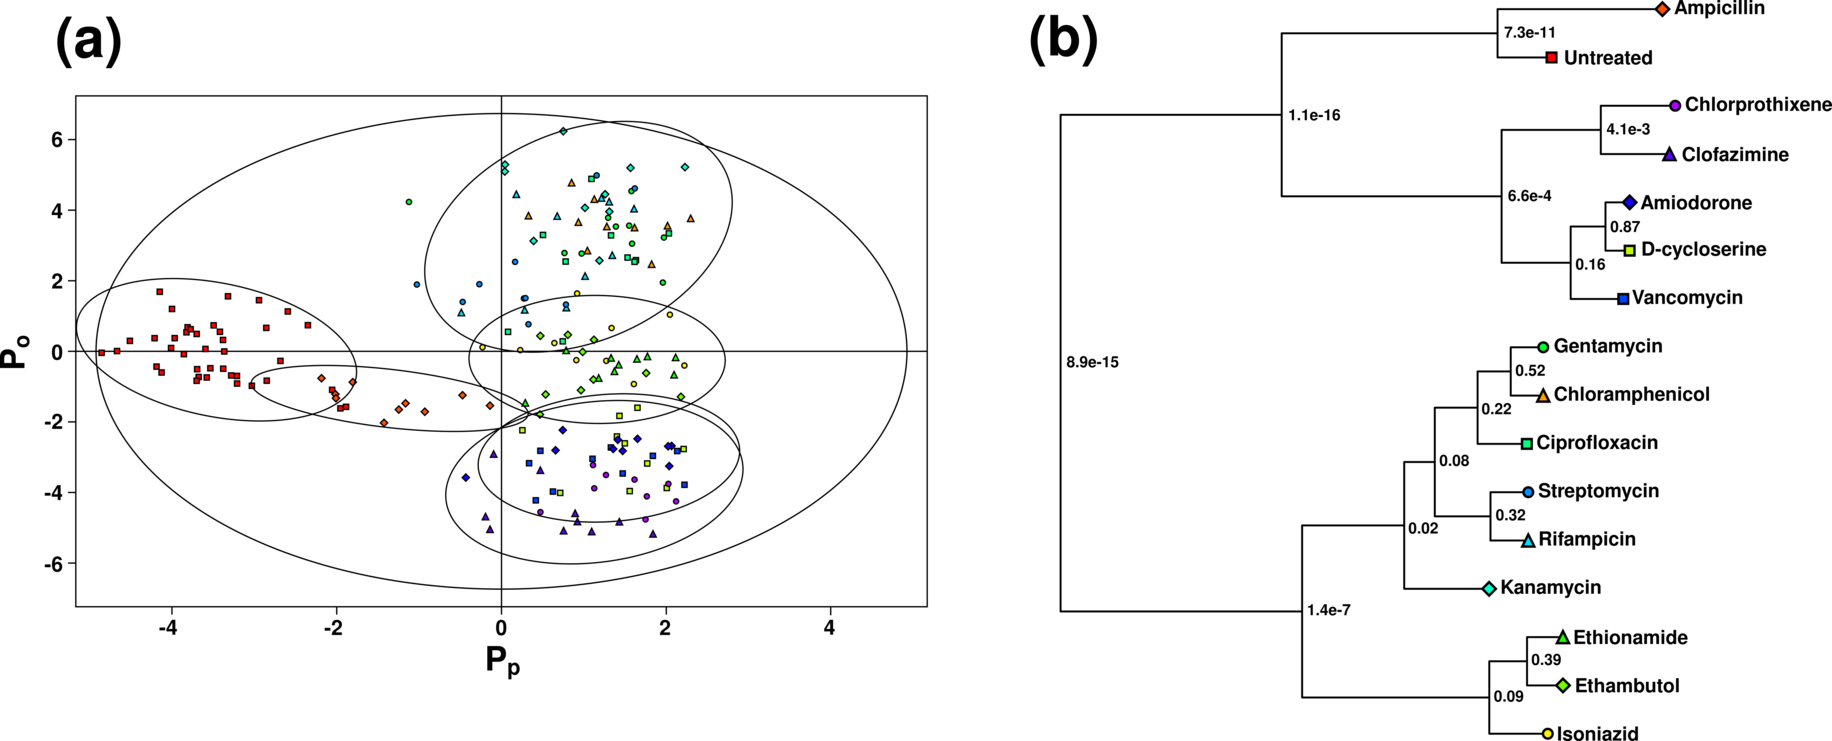
\includegraphics[width=6.5in]{figs/utils/01.png}
\caption
      [Confidence Ellipses and $p$-dendrogram of Example OPLS-DA Scores.]{
  {\bf Confidence Ellipses and $p$-dendrogram of Example OPLS-DA Scores.}
  \\
  ({\bf A}) 2D OPLS-DA scores plot illustrating 95\% confidence ellipses for
  a model having one predictive (PLS) and one orthogonal (OSC) component. The
  symbol shape and color each point correpond to the groups in ({\bf B}).
  Discrimination in the first component is between wild-type and
  antibiotic-treated {\it Mycobacterium smegmatis}, and separations along the
  second component indicate metabolic differences between different antibiotic
  treatments. The antibiotics cluster together based on a shared biological
  target (cell wall synthesis, mycolic acid biosynthesis, or transcription,
  translation and DNA supercoiling). ({\bf B}) Dendrogram generated from the
  scores in ({\bf A}) using Mahalanobis distances, with $p$ values for the null
  hypothesis reported at each branch.
}
\end{figure}

\subsection{Dendrogram Generation}

\begin{doublespace}
The implementation of the tree-generation procedure is a classical UPGMA
algorithm \cite{sokal:uksci1958}. When $p$ values are reported at
each branch point, a single tree is generated based on the matrix of
Mahalanobis distances between groups. In the case of bootstrapped trees, the
groups are randomly resampled with replacement while preserving group size.
The desired number of trees is then generated using Euclidean distances
between group means. The final tree used to report bootstrap probabilities
is built using a Euclidean distance matrix calculated from the original
(non-resampled) dataset.
\end{doublespace}

\subsection{Confidence Ellipse Calculation}

\begin{doublespace}
When viewing PCA and PLS-DA scores plots, it was common practice to apply
hand-drawn ellipses to inform group membership, or even to omit such ellipses
entirely. This may lead to inconsistent or erroneous interpretation of
experimental results. Instead, the fact that the Mahalanobis distances of a
set of $p$-variate points from their sample mean follow a $\chi^2$ distribution
having $p$ degrees of freedom \cite{hotelling:ams1931} may be leveraged
to estimate 95\% confidence ellipses for scores in any number of dimensions.
The sample mean $\mathbf{u}$ and sample covariance matrix $\mathbf{S}$ for each
group must first be calculated from its scores-space data. Then, each group
covariance matrix is decomposed into its eigenvalues and eigenvectors,

\begin{equation}
\mathbf{S} = \mathbf{Q} \mathbf{\Lambda} \mathbf{Q}^{-1}
\end{equation}

where $\mathbf{Q} \in \mathbb{R}^{p \times p}$ is an orthogonal matrix holding
the eigenvectors of $\mathbf{S}$, and
$\mathbf{\Lambda} \in \mathbb{R}^{p \times p}$ is a diagonal matrix holding the
corresponding eigenvalues of $\mathbf{S}$.

For the case of two-dimensional scores data, the 95\% confidence ellipse for a
group is as follows:
\end{doublespace}

\begin{equation}
\begin{bmatrix}
x(t) \\
y(t)
\end{bmatrix}
 = \mathbf{u} + \mathbf{Q} \sqrt{\mathbf{\Lambda} F_{0.95,2}^{-1}}
\begin{bmatrix}
\cos(t) \\
\sin(t)
\end{bmatrix}
\end{equation}

\begin{doublespace}
where $F_{0.95,2}^{-1}$ is the value of the inverse $\chi^2$ cumulative
distribution function at $\alpha = 0.05$ and two degrees of freedom, and the
square-root is taken element-wise over $\mathbf{\Lambda}$. Similarly, a
three-dimensional (3D) confidence ellipsoid may be obtained from the
following parametric equation:
\end{doublespace}

\begin{equation}
\begin{bmatrix}
x(u,v) \\
y(u,v) \\
z(u,v)
\end{bmatrix}
 = \mathbf{u} + \mathbf{Q} \sqrt{\mathbf{\Lambda} F_{0.95,3}^{-1}}
\begin{bmatrix}
\cos(u) \cos(v) \\
\cos(u) \sin(v) \\
\sin(v)
\end{bmatrix}
\end{equation}

\begin{doublespace}
where the parameters $t$, $u$ and $v$ are all evaluated on $(0,2\pi)$. These
methods allow for the inclusion of confidence regions onto two- and
three-dimensional scores plots that reflect the 95\% membership boundaries
for each group. The approach assumes normally distributed within-group errors.
Figures 7.1A and 7.2 illustrate the inclusion of these group confidence regions
in representative PCA and OPLS-DA scores, respectively. The ellipses and
ellipsoids clearly define statistically significant class separation and also
provide an example in which multiple groups actually belong to the same
underlying biological classification.
\end{doublespace}

\begin{SCfigure}
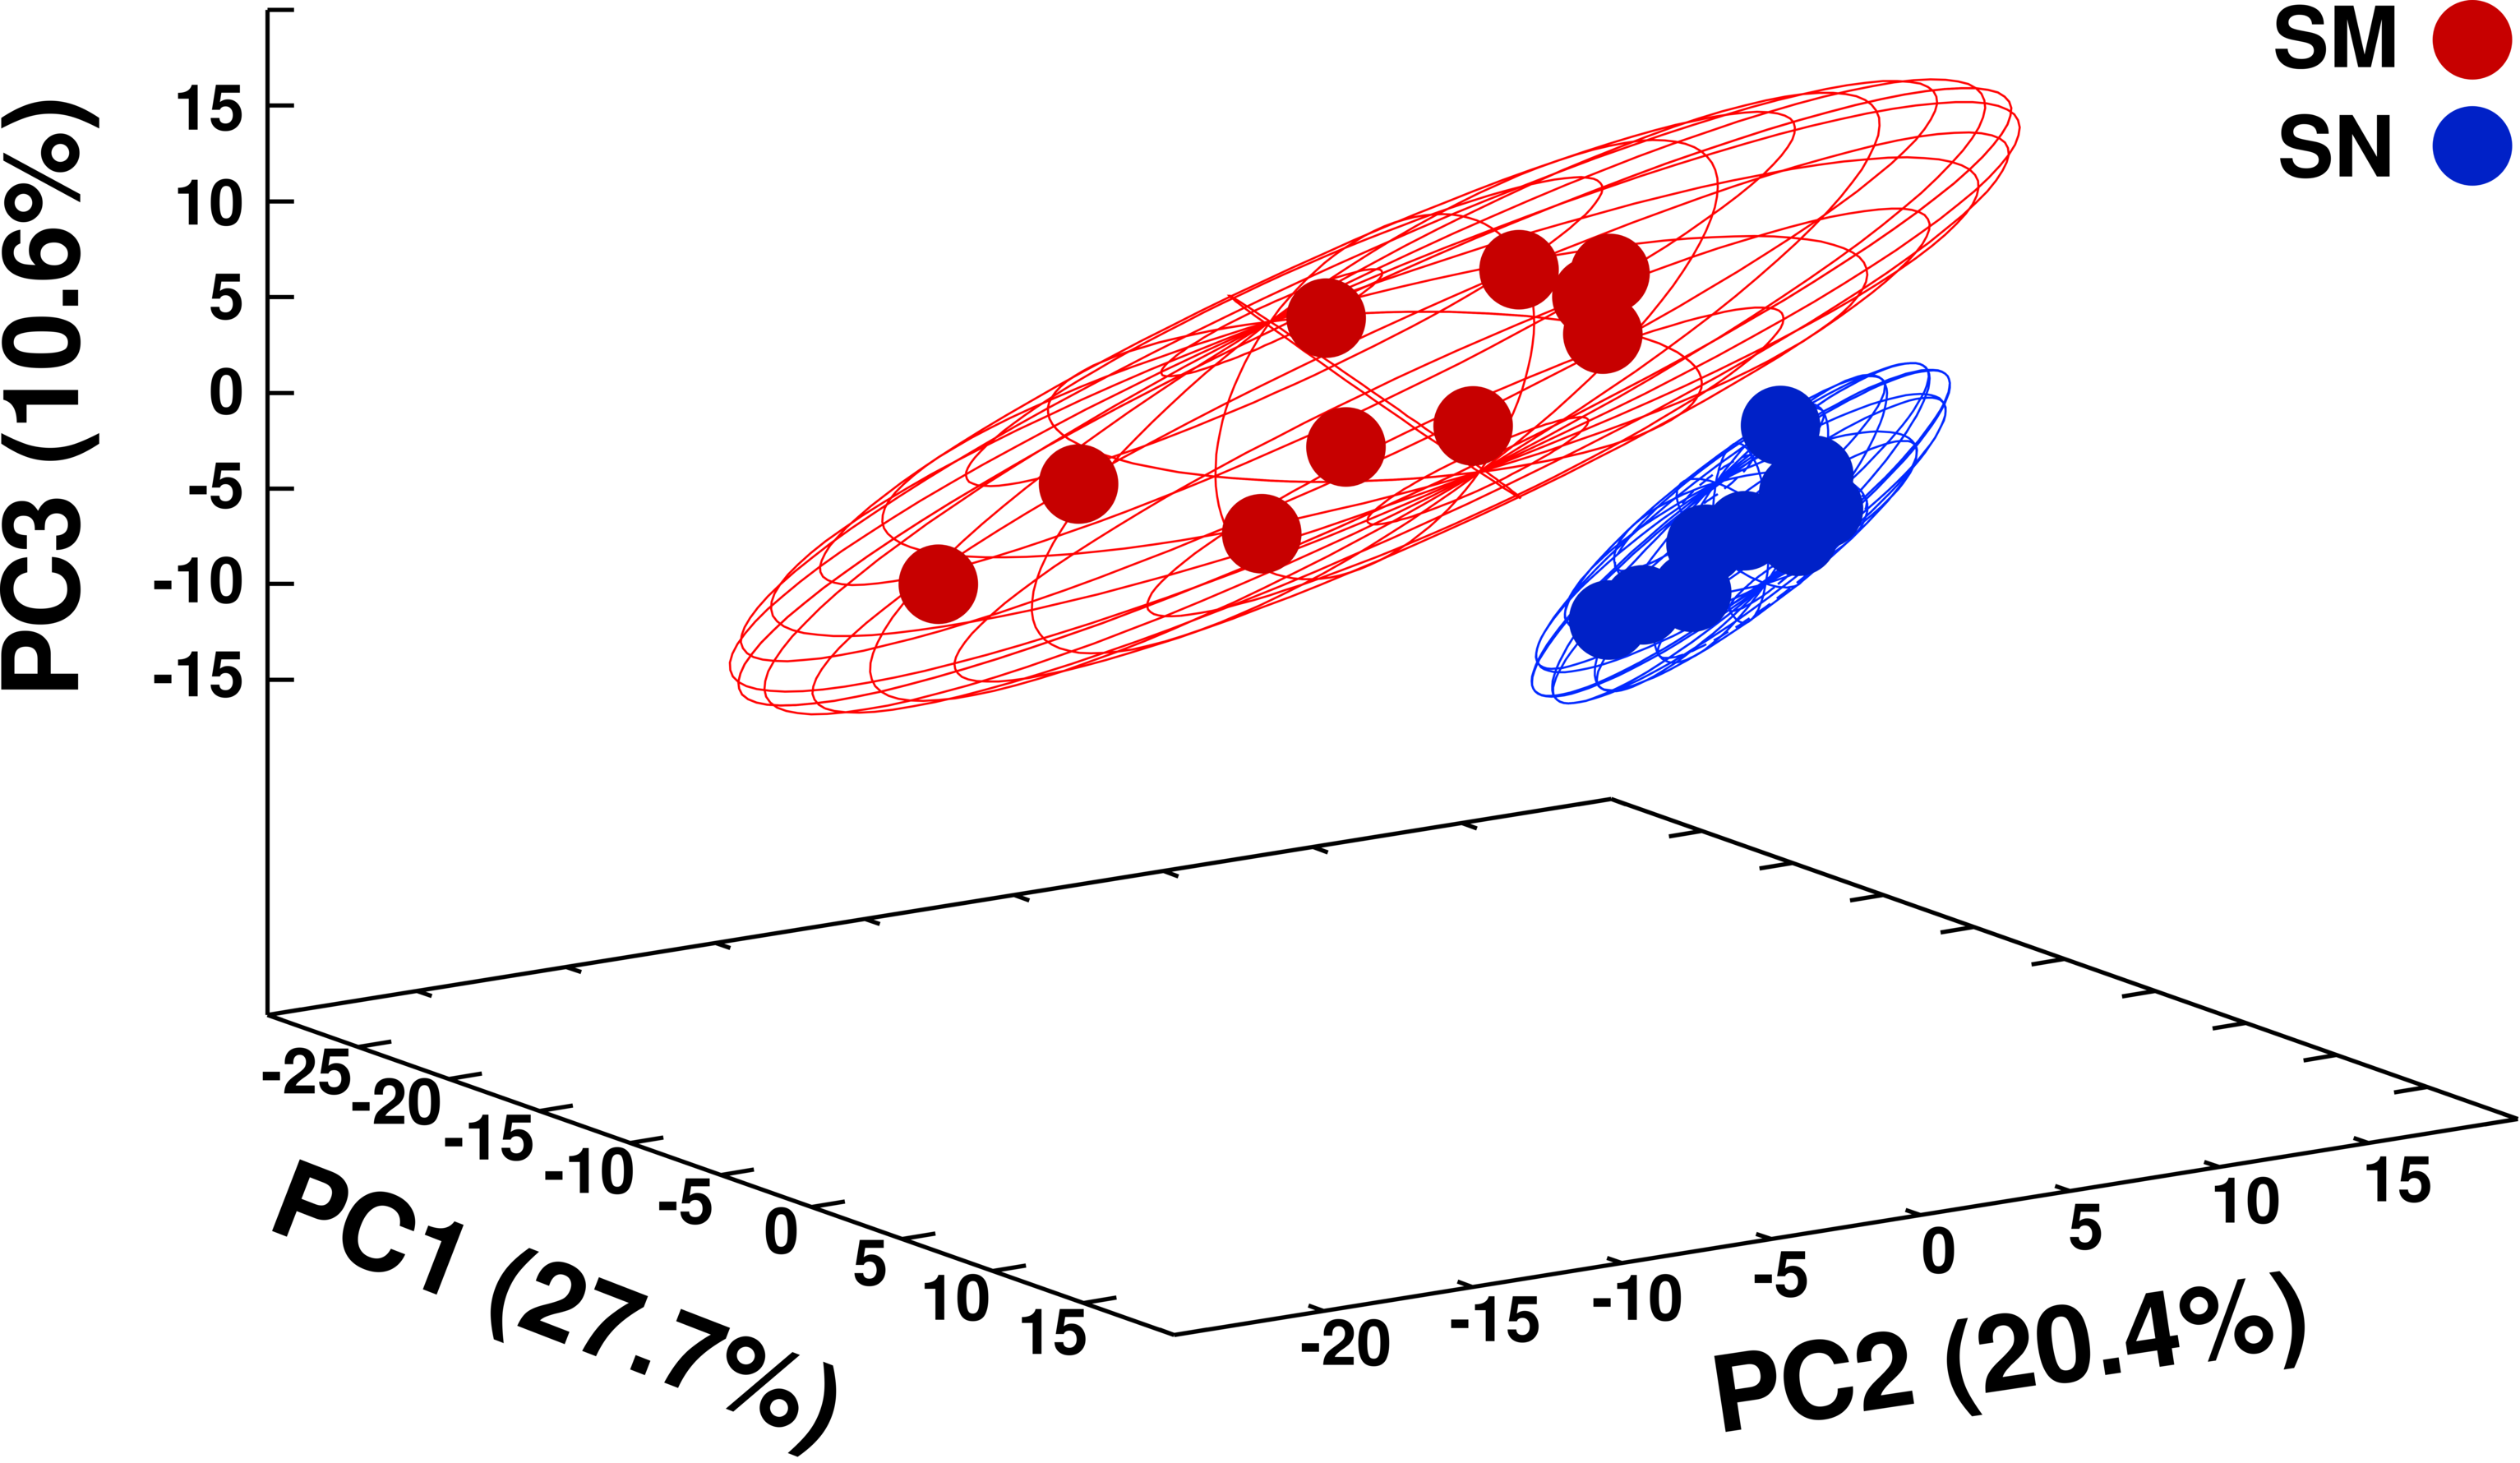
\includegraphics[width=3.5in]{figs/utils/02.png}
\caption
      [Confidence Ellipsoids from PCA Scores.]{
  {\bf Confidence Ellipsoids from PCA Scores.}
  \\
  3D PCA scores plot with superimposed 95\% confidence ellipsoids drawn as
  meshes containing group points. The ellipsoids define the statistical
  significance of class separation and provide an illustration where two
  groups are distinct in three-dimensional scores space.
}
\end{SCfigure}

\section{Results and Discussion}

\begin{doublespace}
The described PCA utilities software package consists of a set of standalone
C programs that generate dendrograms from PCA, PLS-DA and OPLS-DA scores,
report $p$ values and boostrap numbers on tree branches, and incorporate
confidence ellipses/ellipsoids into scores plots. The $p$ values reported for
every pair of distinct groups in scores space provide a truly quantitative
means to discuss group separations. Support for the generation of dendrograms
with these $p$ values at each branch point is also included as an alternative
answer to the bootstrap for answering the question of tree uniqueness. This
eliminates the prior dependence on PHYLIP \cite{retief:mmbio2000}
reported for the original PCAtoTree \cite{werth:abio2010} software
package. The reporting of $p$ values is complementary to bootstrapping methods
in cases of highly overlapped groups, in that it provides a more direct,
interpretable quantitation of group separation.
\\\\
In comparison with PCAtoTree, the PCA utilities software package now uses
Mahalanobis distances because this metric is more appropriate for multivariate
data. De Maesschalck et al. \cite{demaesschalck:cils2000} provide an
exceptional introduction to the use of Mahalanobis distances with PCA.
Specifically, Mahalanobis distances account for different variances in each
scores-space direction ($t_1$, $t_2$, $t_3$, \emph{etc.}) and are invariant
to scaling transformations. This accounting for variances-covariance structure
ensures that the use of a Mahalanobis distance metric for dendrogram generation
includes cluster shape and orientation in the analysis of group separation.
Also, Mahalanobis distances calculated between groups in PCA scores space will
closely approximate those calculated from the original data matrix while
avoiding possible multicollinearities among the original variables. This is
not true of Mahalanobis distances in PLS or OPLS scores space, because of the
underlying supervision of the PLS algorithm. These features differ from the
Euclidean distance metric, which is a special case of the Mahalanobis metric
that arises when the group covariance matrices equal the identity matrix.
Figure 7.1B illustrates the dendrogram structure based on the use of
Mahalanobis distances determined from a set of scores, and Figure 7.3 shows the
dendrogram structure based on Euclidean distances from the same scores.
\end{doublespace}

\begin{SCfigure}
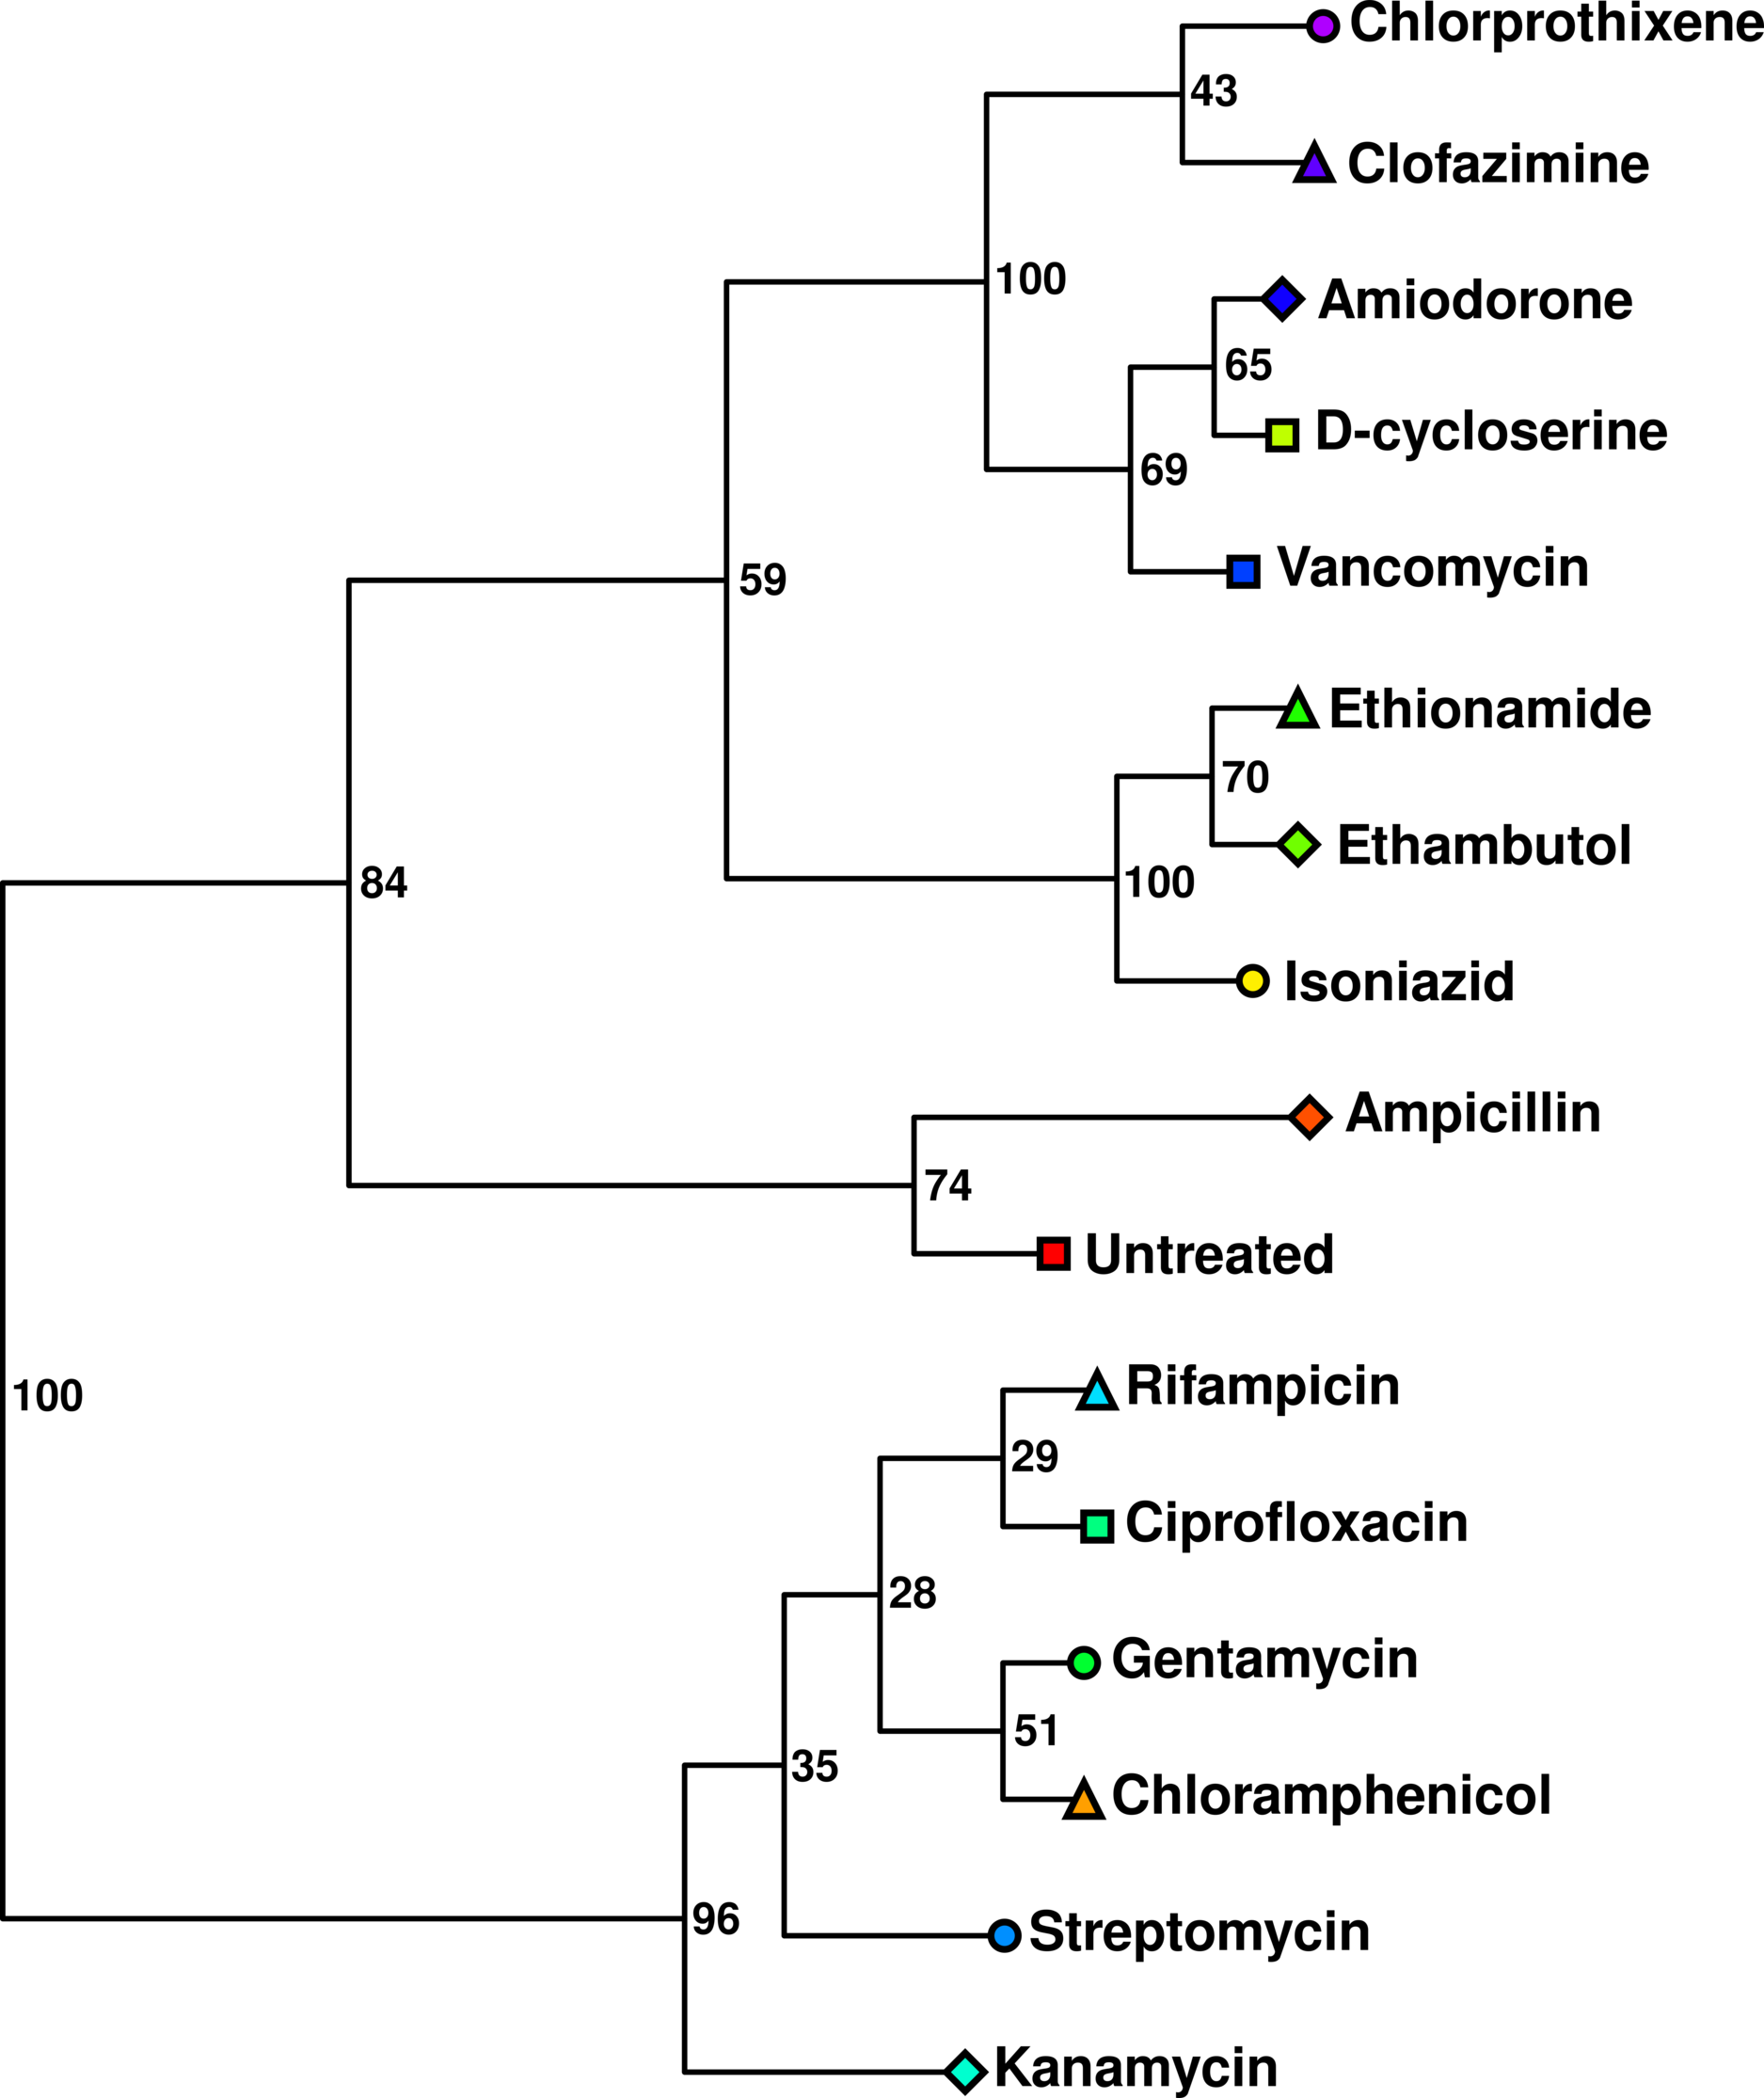
\includegraphics[width=3.5in]{figs/utils/03.png}
\caption
      [Dendrogram Generated using Euclidean Distances.]{
  {\bf Dendrogram Generated using Euclidean Distances.}
  \\
  Bootstrapped dendrogram generated from the scores data in Figure 7.1A using
  a Euclidean distance metric. Bootstrap statistics reported at each branch
  were computed from 5,000 bootstrap iterations.
}
\end{SCfigure}

\begin{doublespace}
It is important to note that our software is not a means of determining the
reliability of PCA or PLS-DA models, but only a toolset for quantifying the
scores that those models produce. In the case of PCA scores, significance of
the principal components used must be inferred based on the explained sum of
squares or another cross-validation technique
\cite{eastment:tech1982,krzanowski:biom1987}. PLS-DA models require
rigorous cross-validation to ensure model reliability, as they almost always
yield perfect separations between the scores of different groups
\cite{kjeldahl:jchemo2010}. With that in mind, separations between
groups not under discrimination may be due to true experimental differences in
PLS-DA scores plots, as opposed to the forced separations between discriminated
groups. Thus, the interpretation of any results from the PCA utilities must be
done with the knowledge of the underlying algorithm's mathematical intent, and
only after the model has been validated. While we demonstrated confidence
region generation using only 2D and 3D scores plots, it is important to note
that the PCA utilities software package places no restriction on the number of
components or on which components may be used during dendrogram generation and
$p$ value calculation. Any dimensionality or choice of scores may be used with
the described methods, provided all components are suitably validated.
\\\\
The updated and enhanced version of PCAtoTree, called PCA utilities, provides
a novel means of quantifying and visualizing separation significance in PCA,
PLS-DA and OPLS-DA scores plots. Importantly, PCA utilities enables single-step
methodologies for generating informative scores plots and dendrograms of
experimental groups in {\it any} study utilizing PCA, PLS-DA or OPLS-DA to
elucidate group structure in complex datasets, including metabolic
fingerprinting and nontargeted metabolic profiling. The tools are distributed
under version 3.0 of the GNU General Public License \cite{gpl3} and are freely
available at \url{http://bionmr.unl.edu/pca-utils.php}.
\end{doublespace}

\bibliographystyle{abbrv}
\bibliography{bworley}



\chapter{Analysis of Protein \npistar{} Interactions}

\begin{quote}
{\it
  Whether you can observe a thing or not depends on the theory which you use.
  It is the theory which decides what can be observed.}
\\\\
 -- Albert Einstein
\end{quote}

\section{Introduction}

\begin{doublespace}
Proteins exhibit a diversity of structures, with 2,738 folds or topologies
present in the CATH database \cite{knudsen:hugen2010}. Each unique
structure is defined by its amino acid composition, where sequence identities
greater than 40\% imply homologous structures \cite{rost:proteng1999}.
Predicting the three-dimensional conformation of a protein from its primary
sequence is a fundamental challenge of structural biology, and achieving this
goal requires a thorough understanding of the underlying interactions and
forces that stabilize protein structures \cite{zhang:opin2008}.
\\\\
Hydrophobic interactions and hydrogen bonds are two of the most common forces
attributed to the overall stability of protein structures
\cite{robertson:chemrev1997,dill:bioc1990}. The burial of hydrophobic
residues is generally considered a major driving force in protein folding
\cite{kauzmann:apc1959} and has been predicted to contribute roughly
8 kJ/mol per buried residue. Conversely, the contribution of hydrogen bonds to
protein structure stability has been controversial
\cite{pace:nsmb2009}. Hydrogen bonds have been described as
destabilizing, partially stabilizing or important driving forces. Of course,
hydrogen bonds are a defining feature of $\alpha$-helices, $\beta$-sheets and
turns. Thus, the generally accepted view is that hydrogen bonds within a
protein structure are marginally favored over hydrogen bonds to water.
Hydrogen bonds are estimated to contribute roughly 4 kJ/mol to protein
stability, but can vary based on the polarity of the microenvironment
\cite{gao:nsmb2009}. Despite these observations, a satisfying
general mechanism for protein folding has not yet been described
\cite{shakhnovich:pnas2009,shaw:sci2010}, which strongly implies
that our understanding of the factors involved in protein folding and stability
is incomplete.
\end{doublespace}

\begin{figure}[ht!]
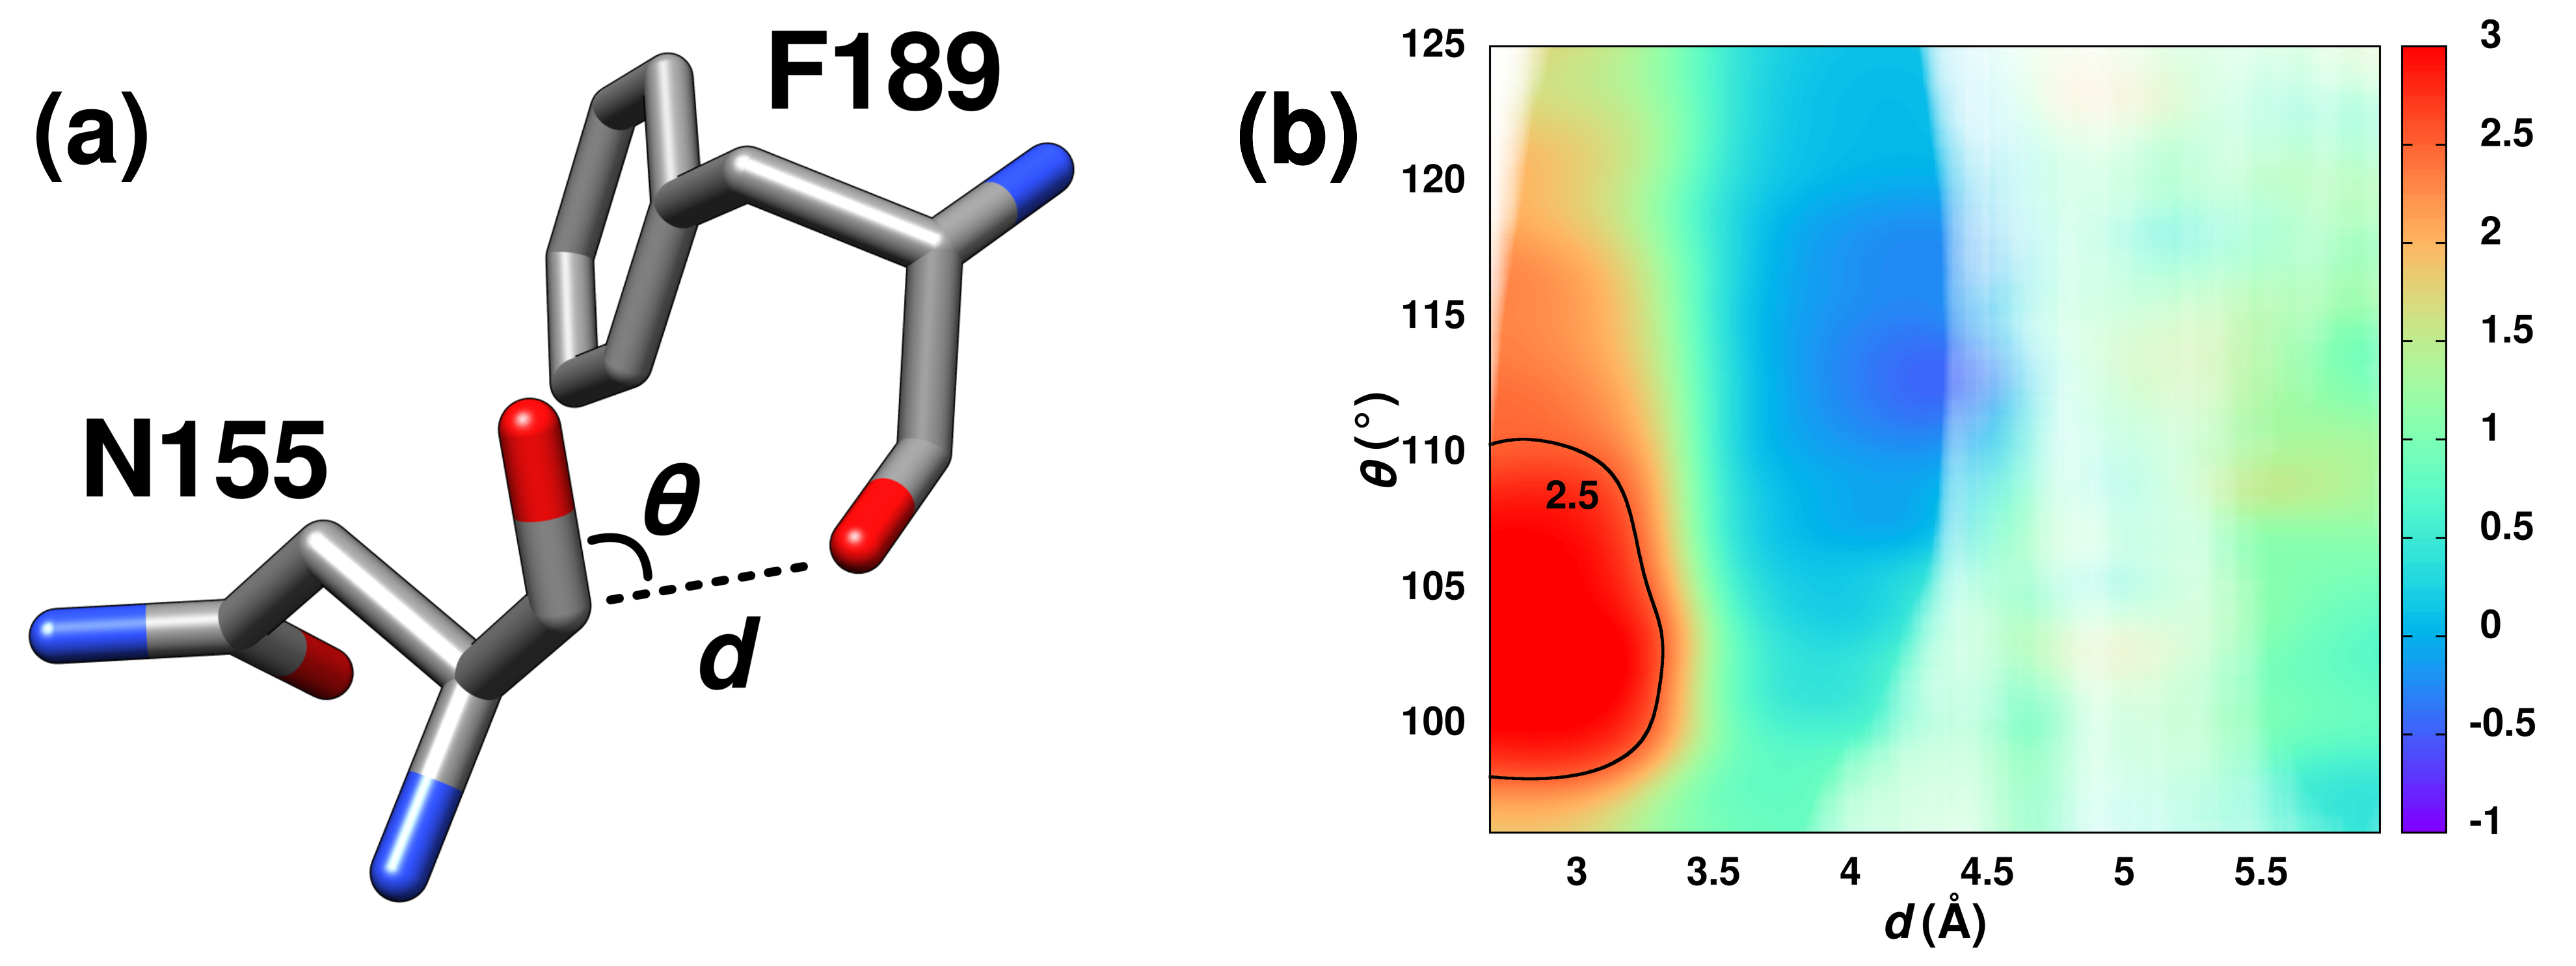
\includegraphics[width=6.5in]{figs/npistar/01.png}
\caption
      [Predicted \npistar{} Interaction and Associated Carbonyl \cnmr{}
       Chemical Shifts.]{
  {\bf Predicted \npistar{} Interaction and Associated Carbonyl \cnmr{}
       Chemical Shifts.
  }
  \\
  ({\bf A}) Residues Asn155 and Phe189 from the x-ray structure of
  \emph{Bacillus amyloliquefaciens} subtillisin BPN' (PDB ID: 1v5i)
  illustrating the structural features for an optimal \npistar{} interaction
  between carbonyl groups.
  ({\bf B}) 2D contour plot of carbonyl \cnmr{} chemical shift differences
  relative to random coil values as a function of the distance ($d$) and
  angle ($\theta$) between carbonyls. A Gaussian smoothing function was
  applied to the data with $\Delta x$ and $\Delta y$ of 0.3 \r{A} and
  1.5$^\circ$, respectively. A transparency mask based on the density of
  experimental data (Figure 8.2) is overlaid on the
  contour plot. Regions lacking experimental data are white.
  Positive values indicate downfield shifts.
}
\end{figure}

\begin{doublespace}
In a recent paper, Bartlett et al. proposed a new and potentially
important interaction analogous to the hydrogen bond
\cite{bartlett:ncb2010}. Unfortunately, the predicted \npistar{}
interaction was based on density functional theory and a relatively low-level
basis set. Conventional Kohn-Sham density functional theory does not properly
model virtual orbitals  \cite{mera:physrev2009} such as the \pistar{}
orbital proposed by Bartlett et al. to have a role in protein stabilization.
Moreover, the relatively low-level basis set used by the authors is inadequate
to model such orbitals, and likely gives rise to substantial basis-set
superposition errors. Experimental data in support of this prediction was also
not presented. Nevertheless, the predicted \npistar{} interaction was suggested
to aid in the stabilization of protein structures and contribute roughly 0.4
to 5.4 kJ/mol. This stabilization was predicted to occur through the electron
delocalization of the lone pair ($n$) of a carbonyl oxygen atom to the
antibonding \pistar{} orbital of a neighboring carbonyl carbon atom. An
optimal \npistar{} interaction was predicted to be restricted to a specific
range of structural parameters (Figure 8.1A) corresponding roughly to the
B\"{u}rgi-Dunitz trajectory \cite{burgi:jacs1973}.
The distance ($d$) between the donor oxygen and acceptor
carbon must be $\leq$ 3.2 \r{A}, and the angle between the
(donor O)$\cdots$(acceptor C) vector and the acceptor carbonyl vector,
$\theta$, must lie between 99$^\circ$ and 119$^\circ$. Interestingly, the
structural parameters required for an optimal \npistar{} interaction are
prevalent in a wide variety of common secondary structures, including
$\alpha$-helices, $3_{10}$-helices and twisted $\beta$-sheets, suggesting
a potential alternative explanation.
\\\\
Despite the presence of numerous conformations consistent with the \npistar{}
interaction in protein structures, no experimental evidence was presented
that supported the actual existence of this interaction. NMR chemical shifts of
$sp^2$-hybridized groups contain a paramagnetic component caused by mixing of
excited states with non-zero orbital angular momentum into the diamagnetic
ground state \cite{ramsey:physrev1950}. These excitations are
predominantly \npistar{} and \pipistar{} and are therefore highly sensitive to
perturbations of these orbitals. The predicted \npistar{} interactions between
neighboring carbonyls would be expected to modify the local electronic
environment of the acceptor carbonyl carbon nucleus, and the NMR \cnmr{}
chemical shift of the acceptor carbonyl carbon would experience a significant
chemical shift change in the presence of an \npistar{} interaction
\cite{abragam1961}. Indeed, a strong (roughly 20 ppm range) linear
relationship has been previously observed between carbonyl \cnmr{} chemical
shifts and the carbonyl \npistar{} transition energy
\cite{savitzky:anchem1964,de:mphys1970}.
\\\\
An extensive analysis of \cnmr{} chemical shifts correlated to high-resolution
x-ray structures combined with a detailed analysis of the molecular orbitals of
a formamide trimer model complex does not support the postulated \npistar{}
interaction. In fact, our model indicates that an \npistar{} interaction is
implausible. Instead, a simple dipole-dipole interaction better explains the
observed effects used in support of the \npistar{} interaction. While a prior
manuscript by the same authors dismissed the dipole-dipole interaction
explanation without elaboration \cite{choudhary:jacs2009}, this
work suggests it is a more plausible explanation of the observed data.
\end{doublespace}

\section{Materials and Methods}

\subsection{Analysis of Experimental Structures}

\begin{doublespace}
A detailed statistical analysis was performed to correlate experimentally
observed carbonyl \cnmr{} chemical shifts with structural parameters between
all possible pairs of carbonyls. Specifically, the angle between the carbonyls
($\theta$) and the distance ($d$) between the oxygen and carbon were compared
to experimental carbonyl \cnmr{} chemical shifts. The PISCES
\cite{wang:binf2003} (\url{http://dunbrack.fcc.edu/pisces}) set of
2,885 high-resolution ($<$ 1.6 \r{A}) x-ray crystal structures with less than
30\% pairwise sequence identity selected from the RCSB Protein Data Bank
(PDB) \cite{berman:nar2000} was used for this analysis. Each structure
was associated with assigned NMR \cnmr{} and \nnmr{} chemical shifts from the
Biological Magnetic Resonance Bank (BMRB: \url{http://www.bmrb.wisc.edu})
\cite{ulrich:nar2008} by FASTA \cite{pearson:mmbio2000}
sequence alignments. The best match with an E-value $\leq 1.0\times10^{-9}$
and sequence identity $\geq$ 95\% was chosen, where the median E-value was
$3.8\times10^{-40}$ . The aligned \cnmr{} and \nnmr{} chemical shifts were
uniformly referenced with the SHIFTCOR software tool
\cite{wishart:jbnmr2003}. The protein interfaces,
surfaces and assemblies software tool
(PISA, \url{http://www.ebi.ac.uk/pdbe/prot_int/pistart.html})
\cite{krissinel:acryst2004} was used to predict residues involved
in crystal packing interfaces. Residues with B-factors two standard deviations
from the mean within each structure were identified as dynamic. Also, 3,699 NMR
solution structures with PDB depositions cross-linked to the BMRB were
used as a validation dataset, with alignments performed in an identical
fashion to the analyzed x-ray structures.
\end{doublespace}

\begin{SCfigure}
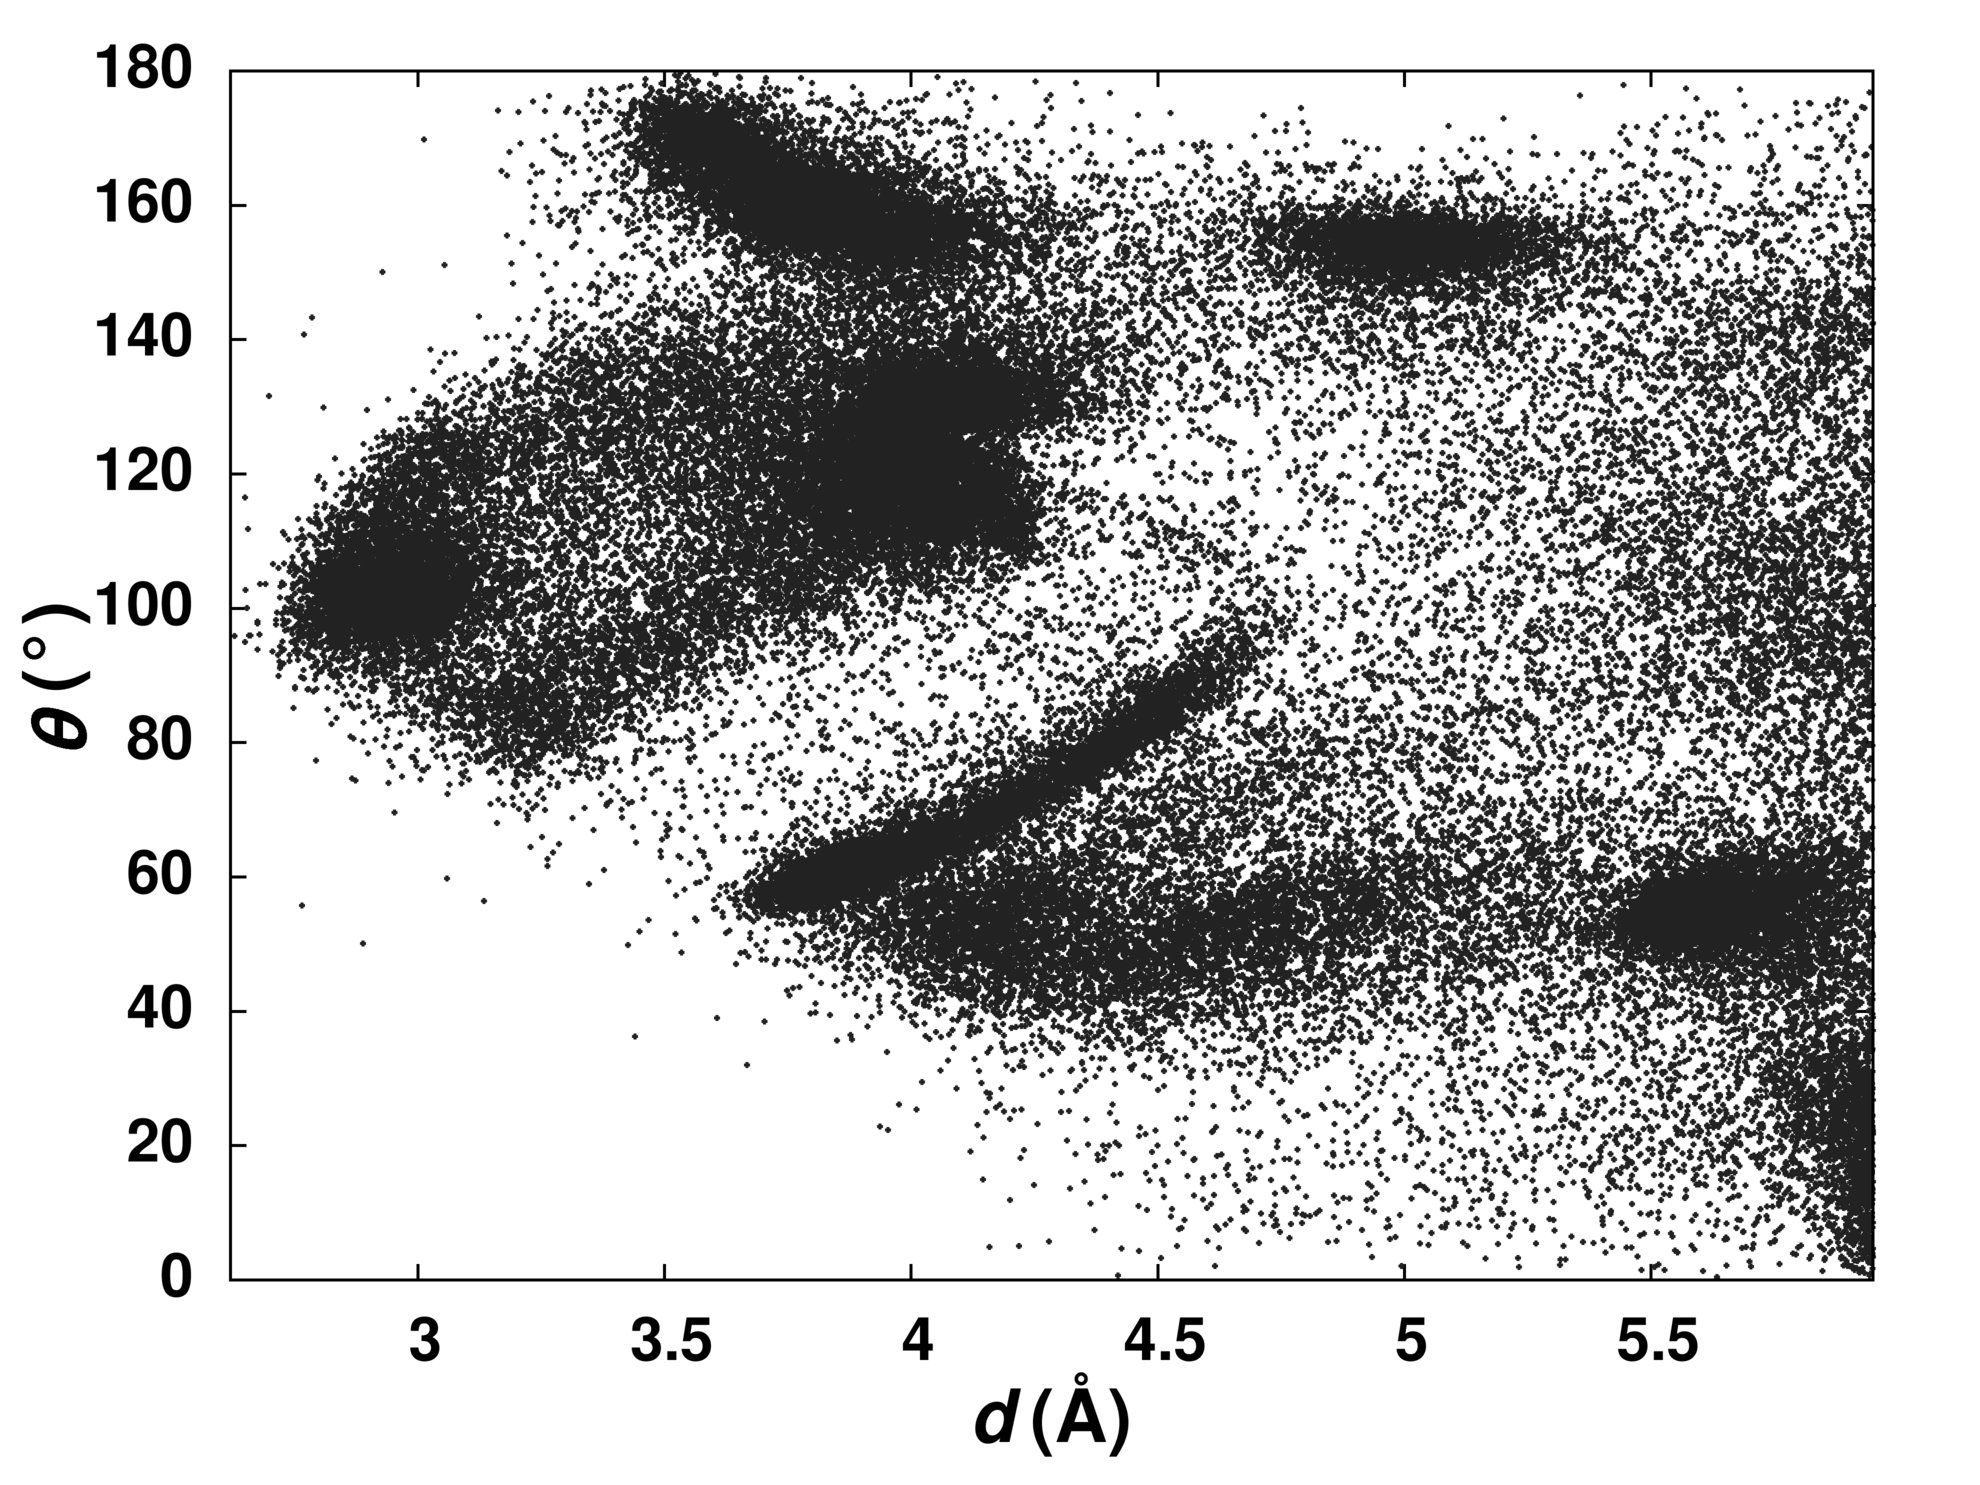
\includegraphics[width=3.5in]{figs/npistar/02.png}
\caption
      [Population of $(d,\theta)$-space by Experimental Structures.]{
  {\bf Population of $(d,\theta)$-space by Experimental Structures.}
  \\
  Plot of the distance ($d$) and angle ($\theta$) measured between each of
  the 45,792 pairs of carbonyls with a potential \npistar{} interaction. The
  relative density of points in the occupied $d$ and $\theta$ space was used
  to generate a transparency mask for Figure 8.1.
}
\end{SCfigure}

\begin{doublespace}
A set of Perl scripts was written to extract structural parameters from
the x-ray structures. For each structure in the selected set, all pairs of
residues were analyzed for the possibility of an \npistar{} interaction. Values
of $d$ and $\theta$ were calculated for each residue pair, and torsional angles
$\phi$ and $\psi$ were calculated for the `acceptor' residue of each pair.
Pairs of carbonyls with $d$ and $\theta$ values within the optimal limits for
an \npistar{} interaction were labeled as interactors (Figure 8.2). Standard
random-coil chemical shifts were subtracted from the experimental carbonyl
\cnmr{} chemical shifts for each residue.
\\\\
For all pairs of residues, a dipole-dipole potential ($V_{dd}$) was calculated
from the high-resolution x-ray structures using equation 8.1:

\begin{equation}
V_{dd} = \frac{
  \vec{\mu}_1 \cdot \vec{\mu}_2 - 3 
    (\vec{\mu}_1 \cdot \hat{r})
    (\vec{\mu}_2 \cdot \hat{r})}{
  4 \pi \epsilon_0 |\vec{r}|^3}
\end{equation}

where $\vec{\mu}_1$ and $\vec{\mu}_2$ are the two C=O bond vectors, $\vec{r}$
is the vector between the centers of the C=O bonds, and $\hat{r}$ is its unit
vector. The nominal value of 2.34 Debye was taken for the carbonyl dipole
moment. Similarly, for all residue pairs, the minimum possible hydrogen bond
length ($d_{O-H}$) was calculated from the high-resolution x-ray structures.
Hydrogen bond lengths were calculated based on the nearest non-neighboring
backbone amide hydrogen, with a maximal bonding angle of 60$^\circ$. Figure
8.3 illustrates the relationship between $V_{dd}$ and \cnmr{} chemical shifts
of all carbonyl pairs in the dataset.
\end{doublespace}

\begin{SCfigure}
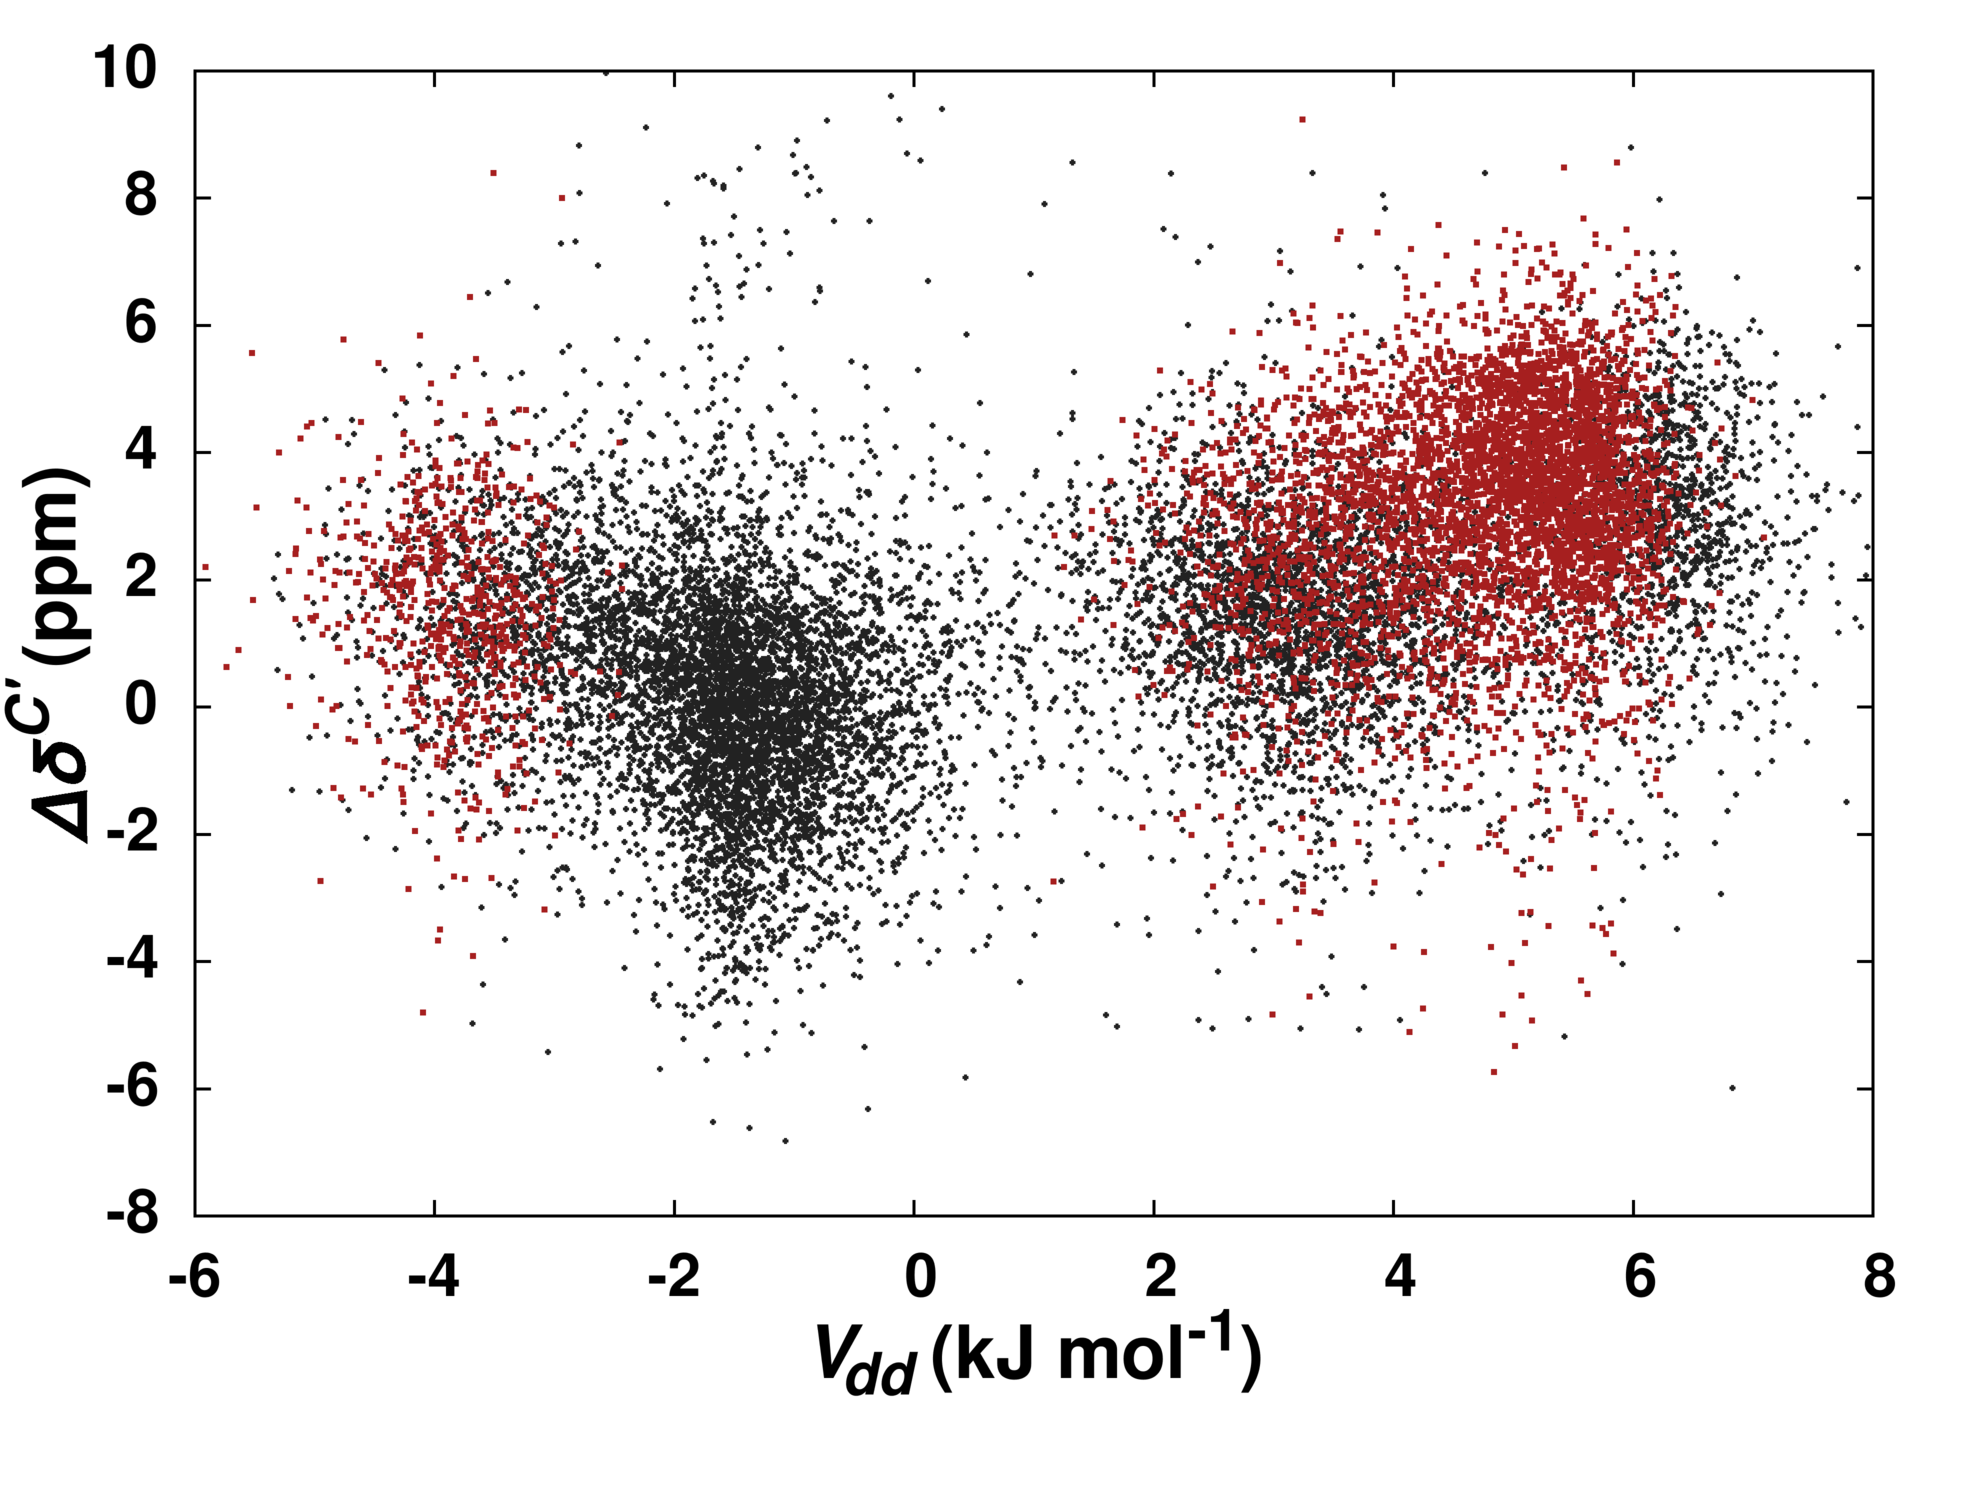
\includegraphics[width=3.5in]{figs/npistar/03.png}
\caption
      [Carbonyl \cnmr{} Chemical Shifts and Dipole-Dipole Potential.]{
  {\bf Carbonyl \cnmr{} Chemical Shifts and Dipole-Dipole Potential.}
  \\
  Carbonyl \cnmr{} chemical shift differences relative to random coil are
  plotted against calculated dipole-dipole potential ($V_{dd}$). The
  dipole-dipole potential is calculated from the high-resolution x-ray
  structure using equation 8.1. Pairs of carbonyls with $d$ and $\theta$
  values within the optimal limits for an \npistar{} interaction are colored
  red.
}
\end{SCfigure}

\subsection{Model Compound Calculations}

\begin{doublespace}
Quantum chemical calculations were performed using the program Gaussian-09
\cite{gaussian2009}. A nearly planar formamide head-to-tail dimer,
composed of a formamide monomer (molecule 1) hydrogen bonded through its C=O
group to the N-H group of a second, nearly parallel formamide (molecule 2) was
chosen to approximate the hydrogen bonding motif found in both $\alpha$-helices
and antiparallel $\beta$-sheets. The dimer was fully optimized at the
MP2/6-311++G(2d,p) level; M\"{o}ller-Plesset second order perturbation theory
(MP2) was chosen because it is superior in modeling long-range and dispersive
contributions to the electron correlation Hamiltonian. A third formamide
(molecule 3) was then added to generate the putative \npistar{} interaction
with molecule 1, imposing the following constraints:
(1) C$_3$=O$_3\cdots$C$_1$ angle fixed at 90$^\circ$, to ensure the $n_\pi$
orbital of molecule 3 points toward the carbonyl of molecule
1 (2) O$_3\cdots$C$_1$=O$_1$ constrained to a set of fixed angles $\theta$,
ranging from 70$^\circ$ to 120$^\circ$ (3) O$_3\cdots$C$_1$ constrained to
a set of fixed distances $d$, ranging from 2.9 \r{A} to 3.3 \r{A}
(5) O$_1\cdots$N$_2$ constrained to a set of fixed distances, ranging
from 2.8 \r{A} to 3.2 \r{A}, to vary the strength of the hydrogen bond. The
system of three molecules was then subjected to constrained optimization at the
same level as before. The optimized trimolecular system at an angle
$\theta = 90^\circ$ is shown in Figure 8.4. Finally, a full set of shielding
tensors was computed using standard Gauge-independent atomic orbital methods.
\end{doublespace}

\begin{SCfigure}
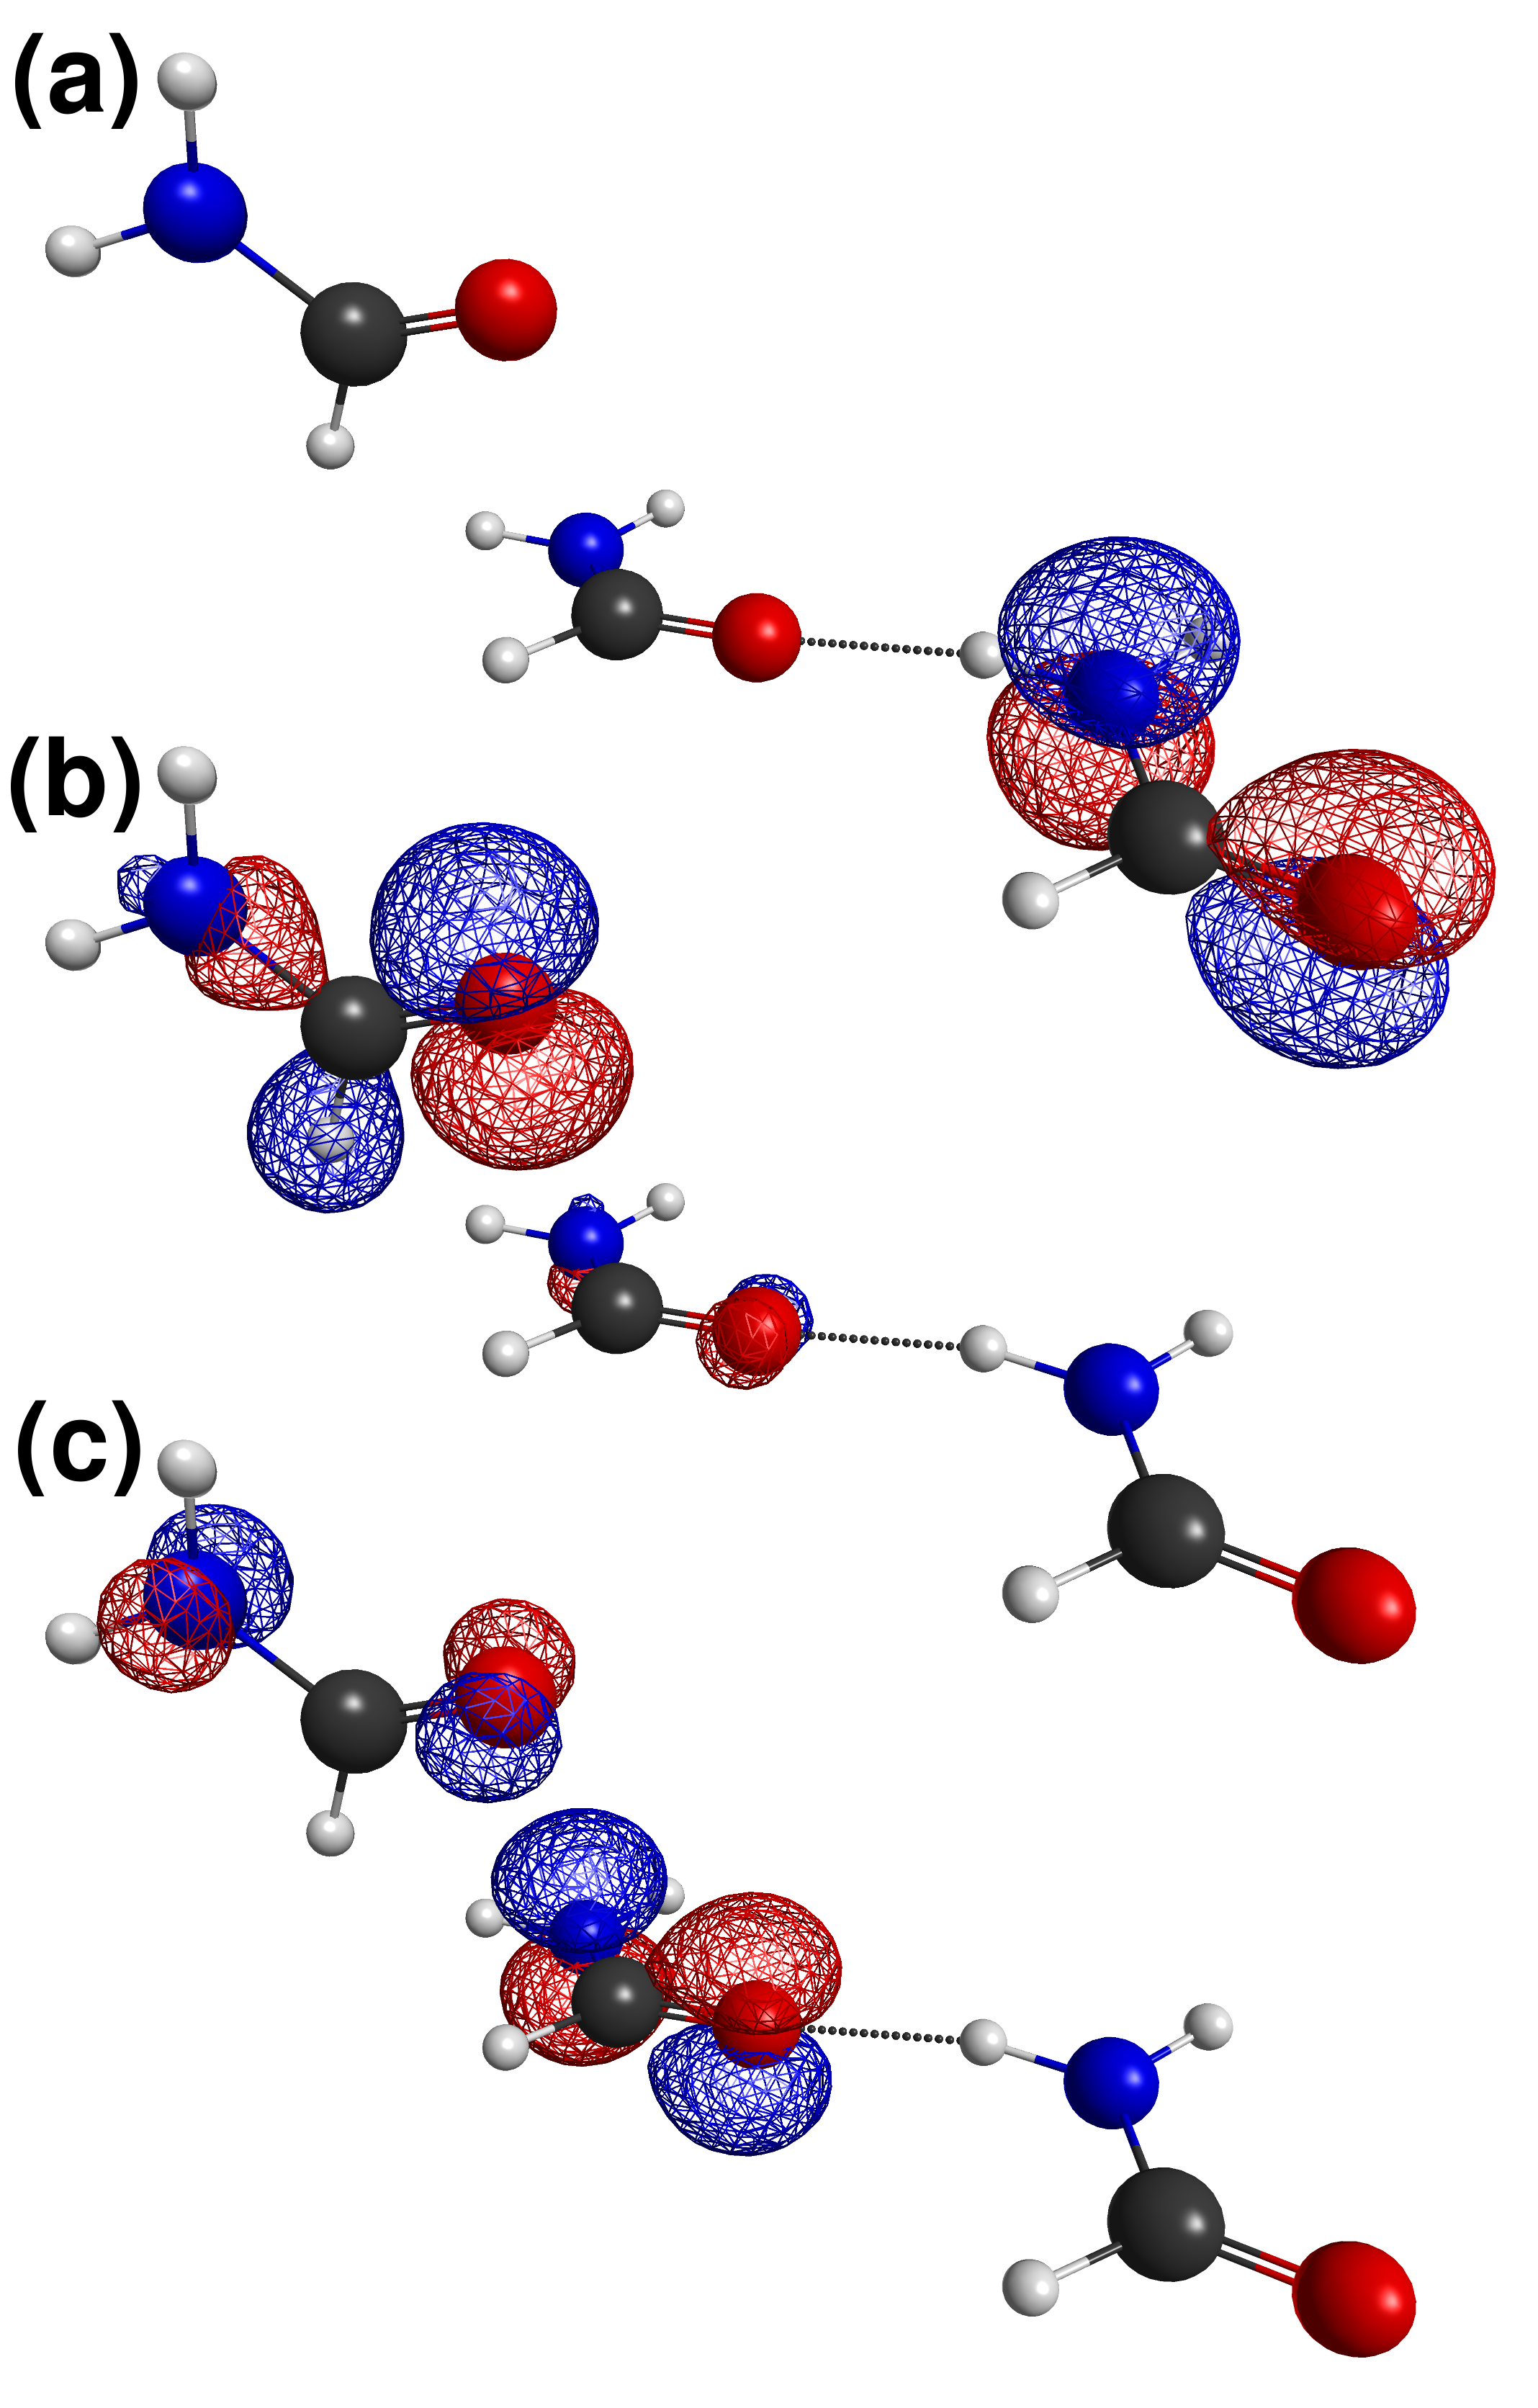
\includegraphics[width=3.5in]{figs/npistar/04.png}
\caption
      [Formamide Trimer Model.]{
  {\bf Formamide Trimer Model.}
  \\
  Molecular orbitals of ({\bf A}) the hydrogen bond donor, ({\bf B}) the
  putative \npipistar{} donor and ({\bf C}) the putative \npipistar{} acceptor,
  in the trimeric complex used in quantum chemical calculations.
}
\end{SCfigure}

\section{Results}

\begin{doublespace}
A total of 2,516,360 residue pairs from a set of 164 high-resolution
($<$ 1.6 \r{A}) x-ray crystal structures with assigned and uniformly referenced
carbonyl \cnmr{} chemical shifts were analyzed for potential \npistar{}
interactions. Setting a maximal distance of 6.0 \r{A} between the donor oxygen
and acceptor carbon yielded 45,792 potential acceptor carbonyl carbon atoms.
The carbonyl \cnmr{} chemical shift differences relative to random coil values
for each of the 45,792 potential acceptor carbonyls were plotted against the
$d$ and $\theta$ values for each carbonyl pair (Figure 8.1B). These chemical
shift differences represent the contribution from the local structural
environment, and potentially the \npistar{} interaction. The two-dimensional
contour plot indicates a maximal downfield shift of 2.9 ppm centered on the
optimal structural parameters predicted for an \npistar{} interaction.
\\\\
Of the 45,792 carbonyls, 5,378 had optimal $d$ and $\theta$ values for an
\npistar{} interaction and 40,414 were outside this optimal range. The mean
carbonyl \cnmr{} chemical shift difference for the 40,414 carbonyls labeled as
non-interactors is 0.58 $\pm$ 1.98 ppm. In contrast, the mean carbonyl \cnmr{}
chemical shift difference for the 5,378 interactors is 2.93 $\pm$ 2.41 ppm. A
Student's t-test indicates the difference of 2.35 ppm between the two means is
statistically significant at the 99.9\% confidence level. To address possible
errors introduced into the analysis by highly dynamic residues in the x-ray
structures, possible carbonyl interactors with B-factors greater than two
standard deviations above the mean were omitted from the dataset. In the
resultant set of 44,302 potential carbonyl interactors, the 2.33 ppm chemical
shift difference was statistically indistinguishable from the original
analysis. Similarly, possible interactors predicted at a 95\% confidence level
to participate in crystal-packing interfaces were also omitted from the
dataset. Again, the corresponding set of interactors yielded a chemical shift
difference of 2.33 ppm, which is still statistically significant at the 99.9\%
confidence level.
\\\\
To address the possiblity that differences between x-ray crystal structures
and NMR solution structures may lead to errors in the analysis, a replicate
analysis was performed on a set of 137 NMR solution structures corresponding
to the same set of \cnmr{} and \nnmr{} chemical shifts used previously.
Structural alignments using MAMMOTH showed a mean rmsd of 1.87 $\pm$ 0.57 \r{A}
between the pairs of x-ray and NMR structures. Of the 1,419,547 resulting
carbonyl pairs from the NMR structures, 38,534 pairs were found to be potential
interactors. Of the carbonyls in that set, 2,510 interactors were found with a
mean carbonyl \cnmr{} chemical shift difference of 2.84 $\pm$ 1.71 ppm. The
remaining 36,024 non-interactors had a mean carbonyl \cnmr{} chemical shift
difference of 1.02 $\pm$ 2.02 ppm. Again, the 1.82 ppm difference between the
two means is statistically significant at the 99.9\% confidence level, 
indicating that differences between x-ray and NMR structures cannot account
for the observed downfield \cnmr{} chemical shift.
\\\\
As predicted, a clear correlation is observed between structural regions
consistent with an optimal \npistar{} interaction and a downfield shift of the
accepting carbonyl \cnmr{} resonance. Interestingly, the potential \npistar{}
interactions were primarily observed between sequential ($|i-j|=1$) carbonyls.
Out of the 164 structures and 2,516,360 residue pairs, only four pairs of
carbonyls exhibited a through-space ($|i-j| > 5$) arrangement consistent with
an optimal \npistar{} interaction. This result implies any protein
stabilization energy obtained from the proposed \npistar{} interaction is
opportunistic, as opposed to a driving force for protein folding. Apparently,
the formation of through-space \npistar{} interactions is simply less favorable
than for other interactions, such as hydrogen bonds or salt-bridges. This also
implies that the predicted energy of 5.4 kJ/mol for an optimal \npistar{}
interaction is an over-estimate.
\\\\
In actuality, an \npistar{} interaction that imparts a stability of 5.4 kJ/mol
would likely fix adjacent pairs of carbonyl groups to preferred torsional
angles in order to maximize this interaction. Correspondingly, the existence
of these highly energetic \npistar{} interactions would likely be detrimental
to properly folding a protein structure. Folding a protein to its native fold
would require distorting the majority of carbonyl pairs away from the ideal
torsion angles for a proper \npistar{} interaction. Only ~12\% (5,378 out of
45,792) of carbonyls from the 164 x-ray structures adopted conformations with
optimal $d$ and $\theta$ values for an \npistar{} interaction. As a result,
folding every protein structure would incur an initial energetic penalty of
nearly 5.4 kJ/mol per carbonyl pair.
\end{doublespace}

\begin{SCfigure}
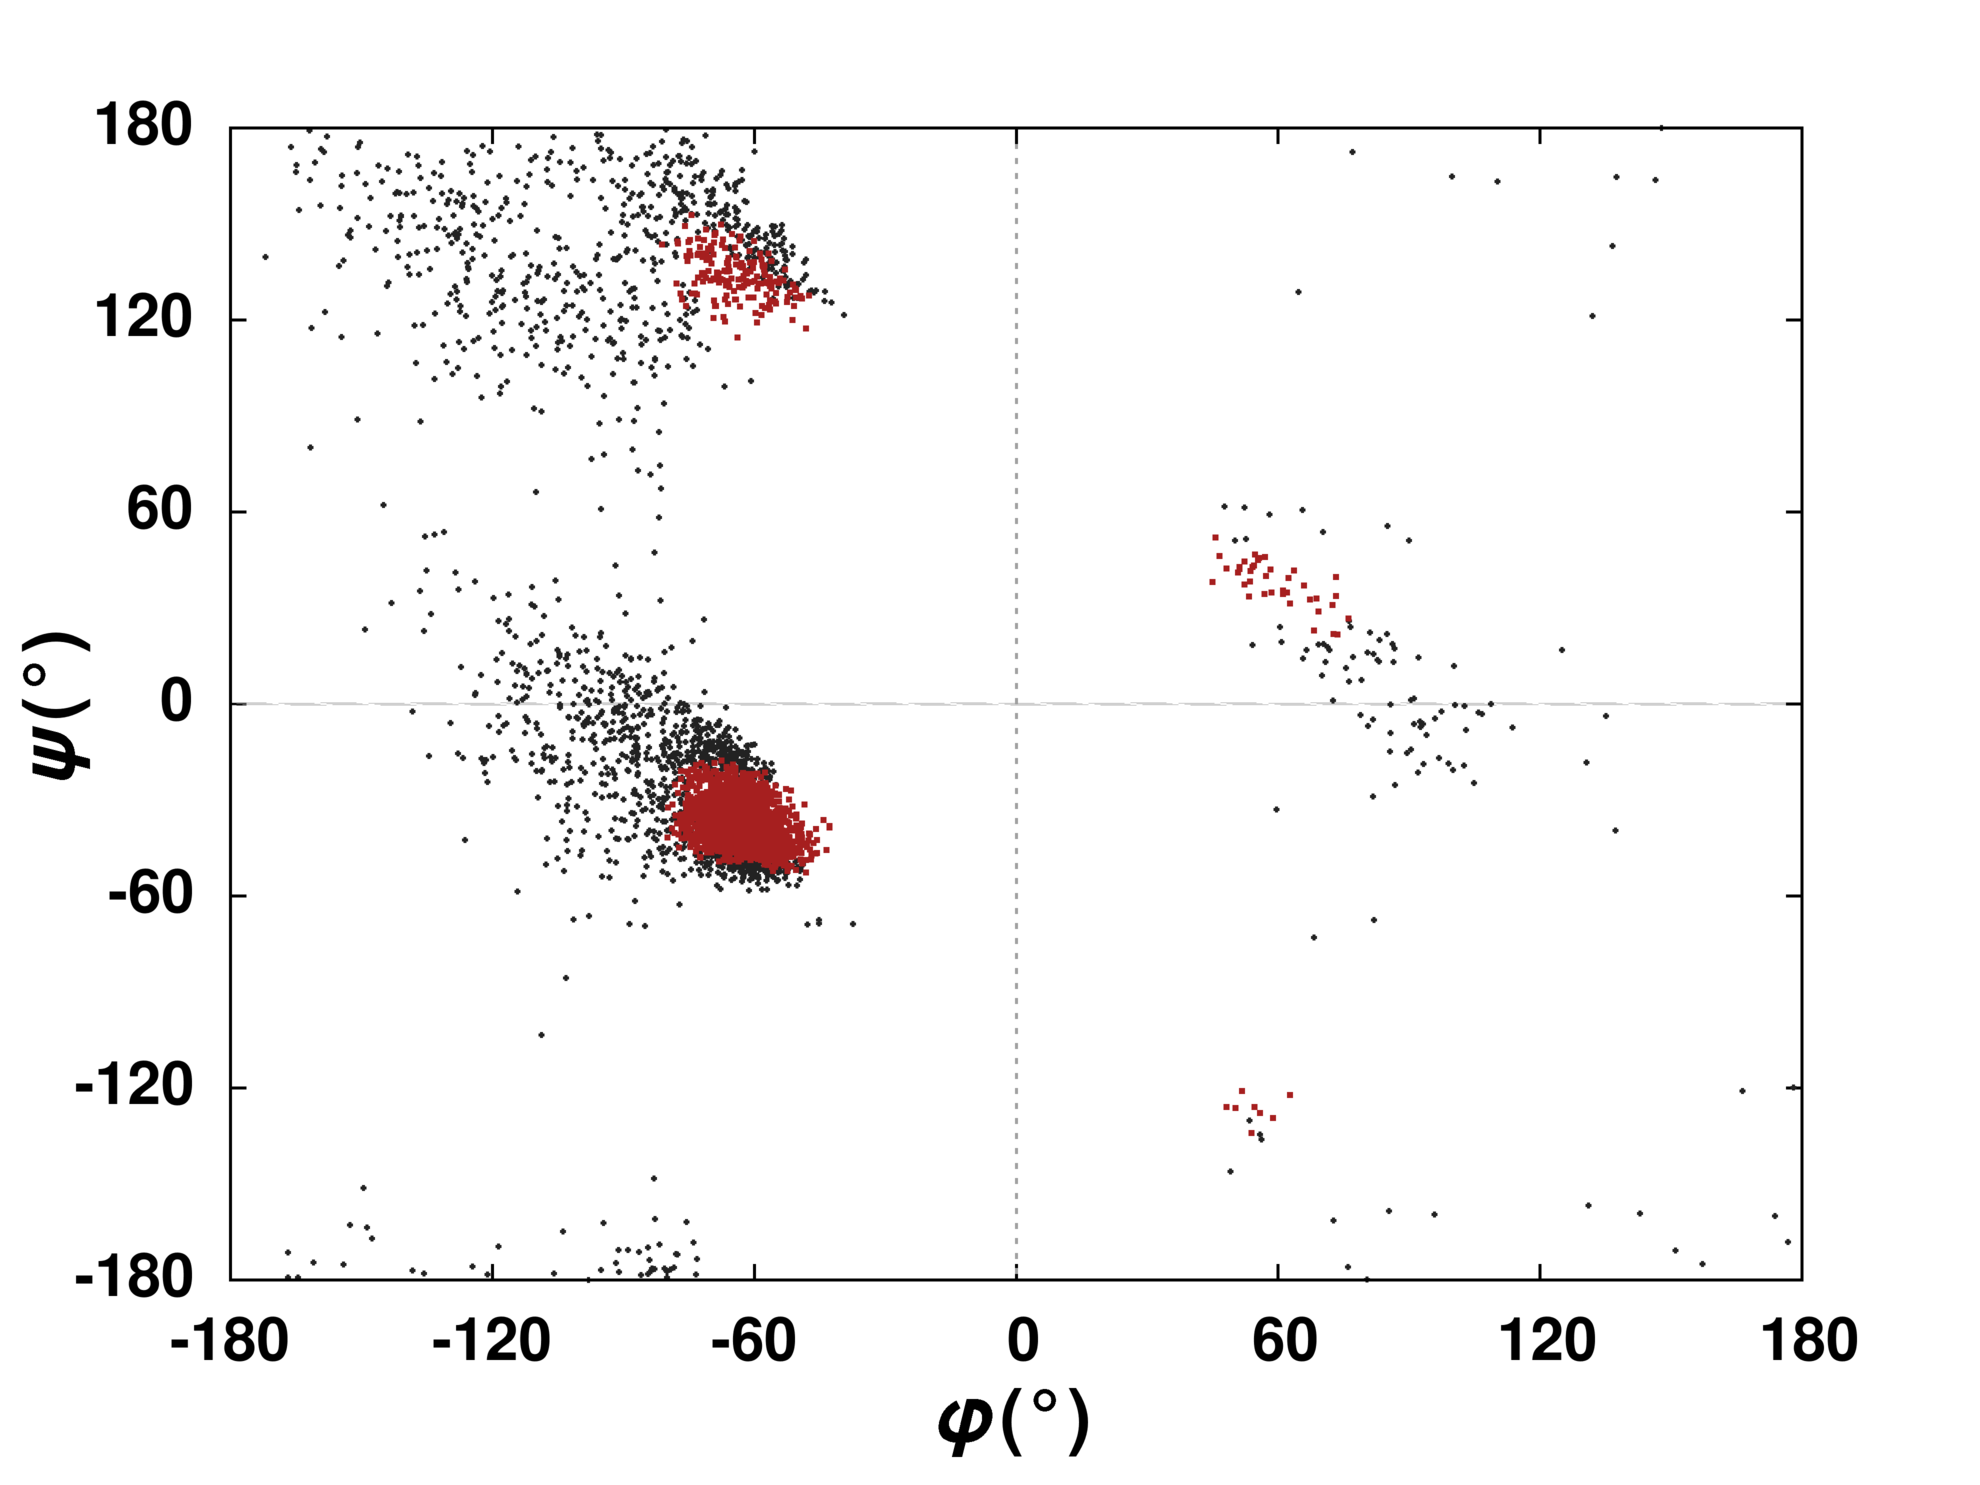
\includegraphics[width=3.5in]{figs/npistar/05.png}
\caption
      [Population of $(\phi,\psi)$-space by Experimental Structures.]{
  {\bf Population of $(\phi,\psi)$-space by Experimental Structures.}
  \\
  Ramachandran plot of carbonyls with \cnmr{} chemical shift differences
  relative to random coil that are $>$ 2.5 ppm. The acceptor carbonyls from
  each pair of carbonyls with $d$ and $\theta$ values within the optimal
  limits for an \npistar{} interaction are colored red.
}
\end{SCfigure}

\begin{doublespace}
A predominant number of the carbonyls consistent with an optimal \npistar{}
interaction and with a downfield shift of roughly 2.5 ppm fall within the
typical $\alpha$-helical region of a Ramachandran plot, where the remaining
residues are near the twisted $\beta$-sheet region (Figure 8.5). Significant
chemical shift changes for carbonyl residues within
secondary structures are well documented \cite{wang:protsci2002}.
Previous analyses of structural factors contributing to carbonyl \cnmr{}
chemical shifts have implicated hydrogen bond formation
\cite{dedios:sci1993,asakawa:jacs1992,wylie:jacs2007}
or excluded hydrogen bond formation
\cite{cisnetti:cpc2004,neal:jbnmr2003,markwick:jacs2004}, have
implicated $\phi$, $\psi$, and $\chi$ dihedral angles
\cite{neal:jbnmr2003} or have excluded secondary structure parameters
\cite{cisnetti:cpc2004,dedios:sci1993}. Thus, other factors,
such as hydrogen bonds or dipole-dipole interactions, may explain the apparent
correlation between carbonyl \cnmr{} shifts and the optimal $d$ and $\theta$
values for an \npistar{} interaction. This is probable given the association of
\npistar{} interactions with secondary structure elements. The contribution of
a dipole-dipole interaction to carbonyl \cnmr{} chemical shifts is illustrated
in Figure 8.3. The dipole-dipole potentials were calculated using the
high-resolution x-ray structures for each of the 45,792 carbonyl pairs with a
maximal distance of 6.0 \r{A} between the donor oxygen and acceptor carbon.
While there is significant scatter in the data, there is also a clear trend
between a downfield carbonyl \cnmr{} chemical shift and an increasing
dipole-dipole energy. Importantly, the cluster of acceptor carbonyls in
Figure 8.3 with the largest \cnmr{} chemical shift difference
(3.15 $\pm$ 2.44 ppm) and positive dipole-dipole potentials also conforms to
the optimal $d$ and $\theta$ values for the predicted \npistar{} interaction.
\end{doublespace}

\begin{SCfigure}
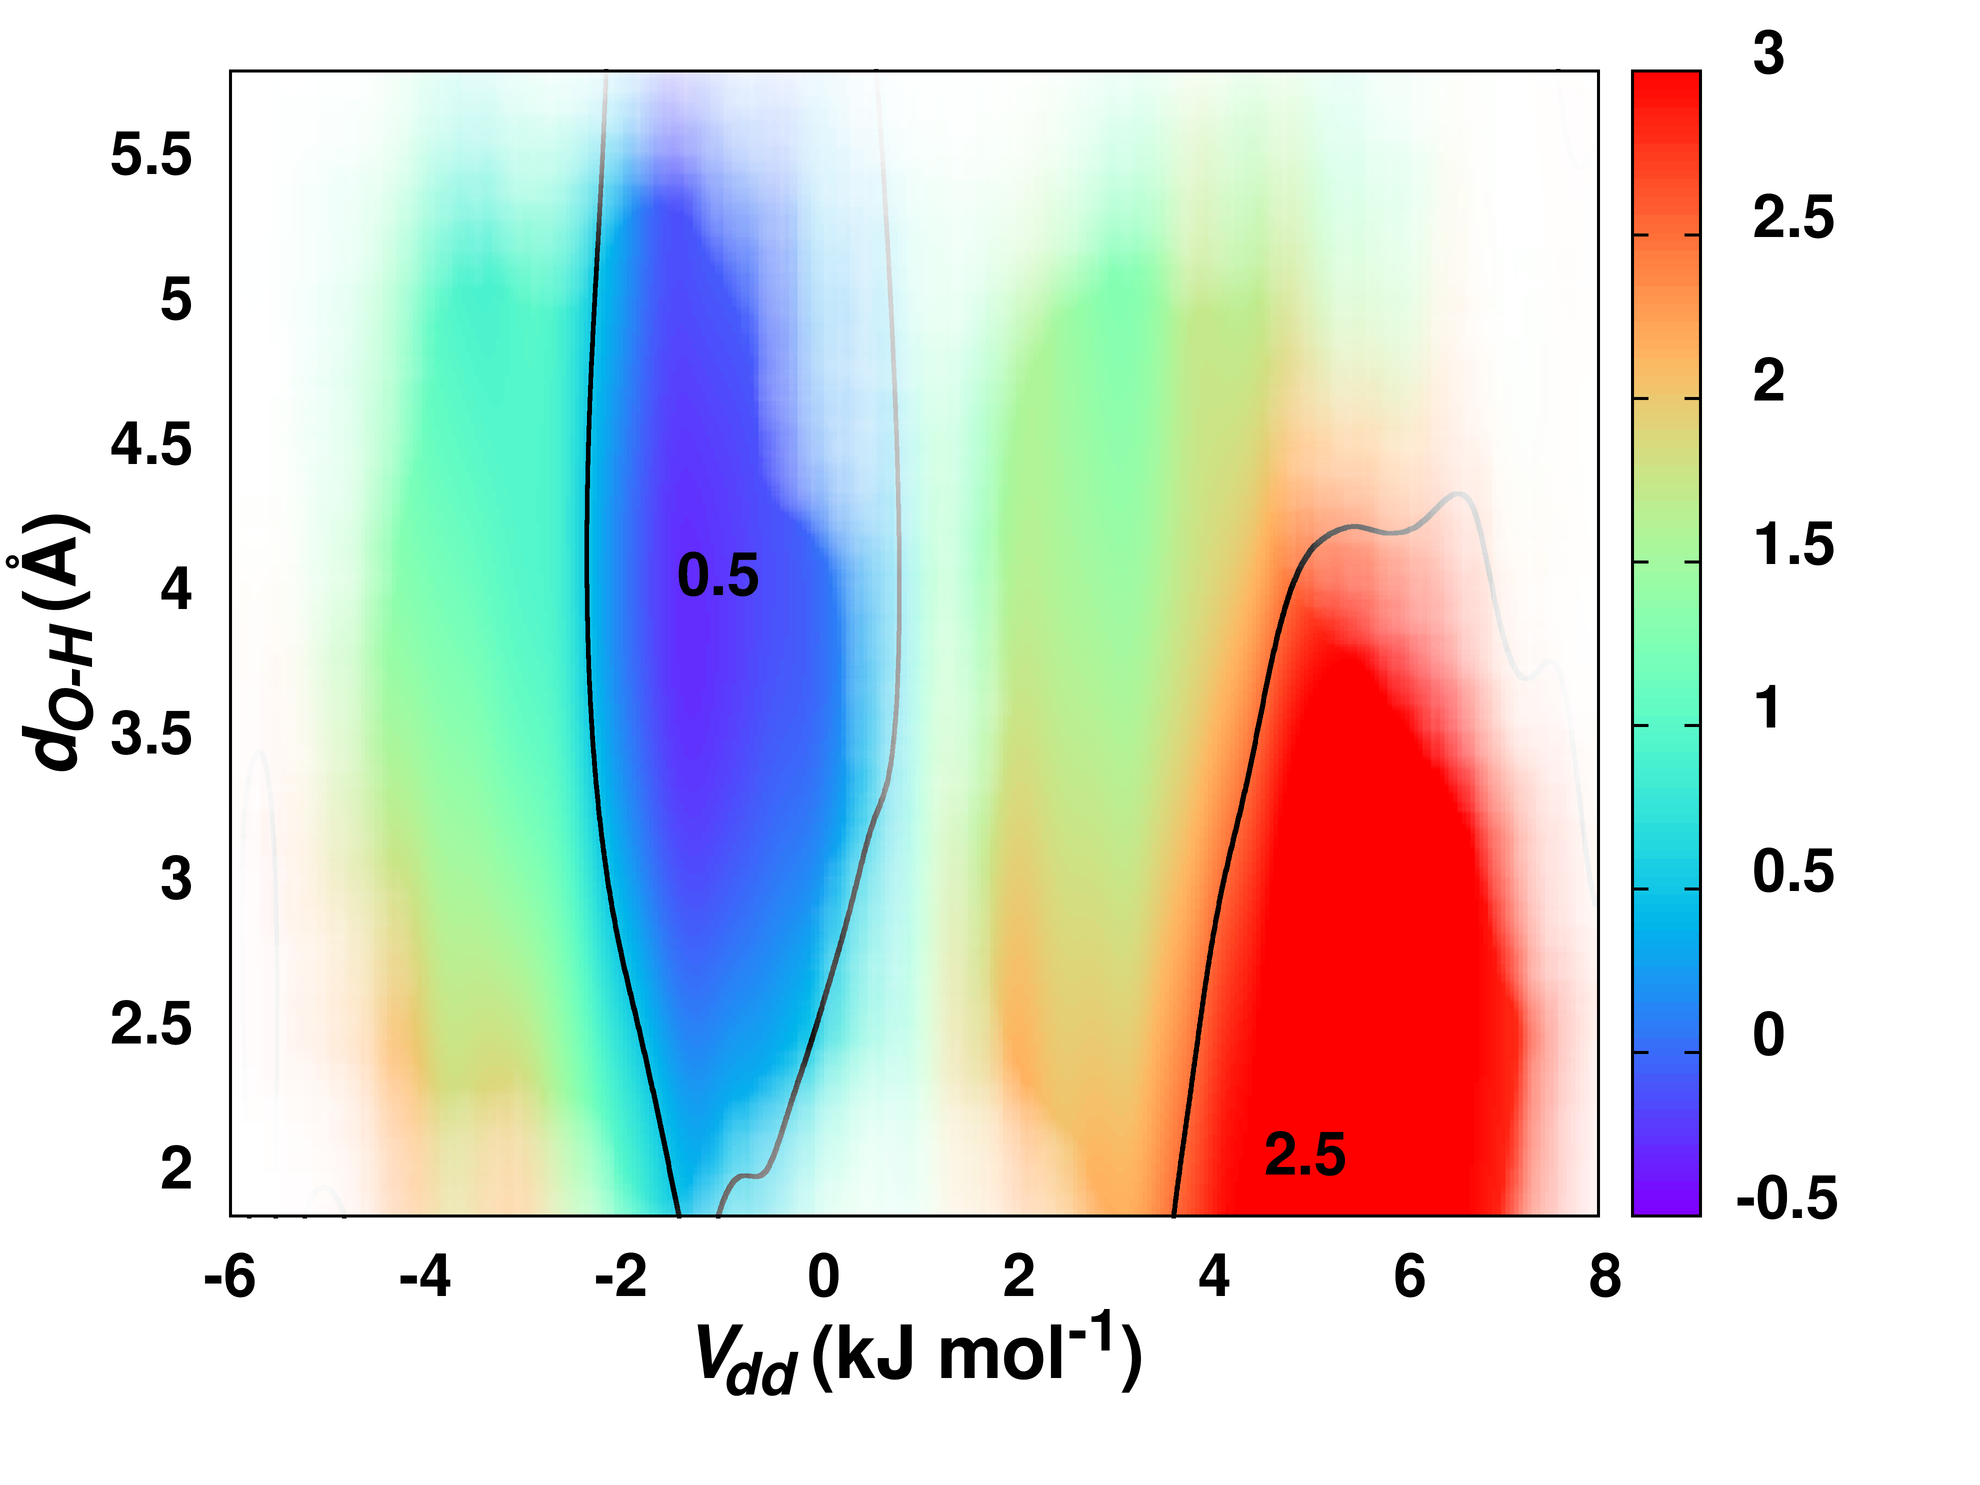
\includegraphics[width=3.5in]{figs/npistar/06.png}
\caption
      [Carbonyl \cnmr{} Chemical Shifts and Hydrogen Bonds.]{
  {\bf Carbonyl \cnmr{} Chemical Shifts and Hydrogen Bonds.}
  \\
  Contour plot of \cnmr{} carbonyl chemical shift differences as a function
  of calculated dipole-dipole potential ($V_{dd}$) and calculated hydrogen
  bond length ($d_{O-H}$).
}
\end{SCfigure}

\begin{doublespace}
The contribution of a hydrogen-bond interaction to the carbonyl \cnmr{}
chemical shift was similarly evaluated by calculating the shortest
oxygen-hydrogen distance ($d_{O-H}$) for each donor carbonyl. Again, the
distances were calculated using the high-resolution x-ray structures for each
of the 45,792 carbonyl pairs. A three-dimensional plot comparing the
dipole-dipole potentials, oxygen-hydrogen distances, and the associated
carbonyl \cnmr{} chemical shifts is very revealing. It can be clearly seen
from Figure 8.6 that any contribution from a hydrogen bond to the \cnmr{}
carbonyl chemical shift is minimal relative to the dipole-dipole contribution.
Both the $\alpha$-helical and $\beta$-sheet regions, which obviously contain
hydrogen bond interactions, have distinctly different \cnmr{} carbonyl chemical
shifts. The $\alpha$-helical region corresponds to a positive dipole-dipole
interaction, and correspondingly to a large carbonyl \cnmr{} chemical shift
difference. Conversely, the $\beta$-sheet region has a negative dipole-dipole
interaction and a near zero carbonyl \cnmr{} chemical shift difference. These
results further indicate a consistency with a dipole-dipole interaction as
opposed to the predicted \npistar{} interaction.
\\\\
It is important to note that there is a second cluster of carbonyls in Figure
8.3 with low \cnmr{} chemical shifts and negative dipole-dipole potentials that
are also consistent with the optimal $d$ and $\theta$ values for the predicted
\npistar{} interaction. A visual inspection of the x-ray structures indicates
that these carbonyl pairs are actually pointing away from each other and do not
form the configuration for an \npistar{} interaction illustrated in Figure
8.1A. Clearly, $d$ and $\theta$ values alone fail to adequately define the
optimal geometry of the dipole-dipole interaction that is apparently
responsible for the observed downfield \cnmr{} chemical shifts.
\end{doublespace}

\begin{figure}[h!]
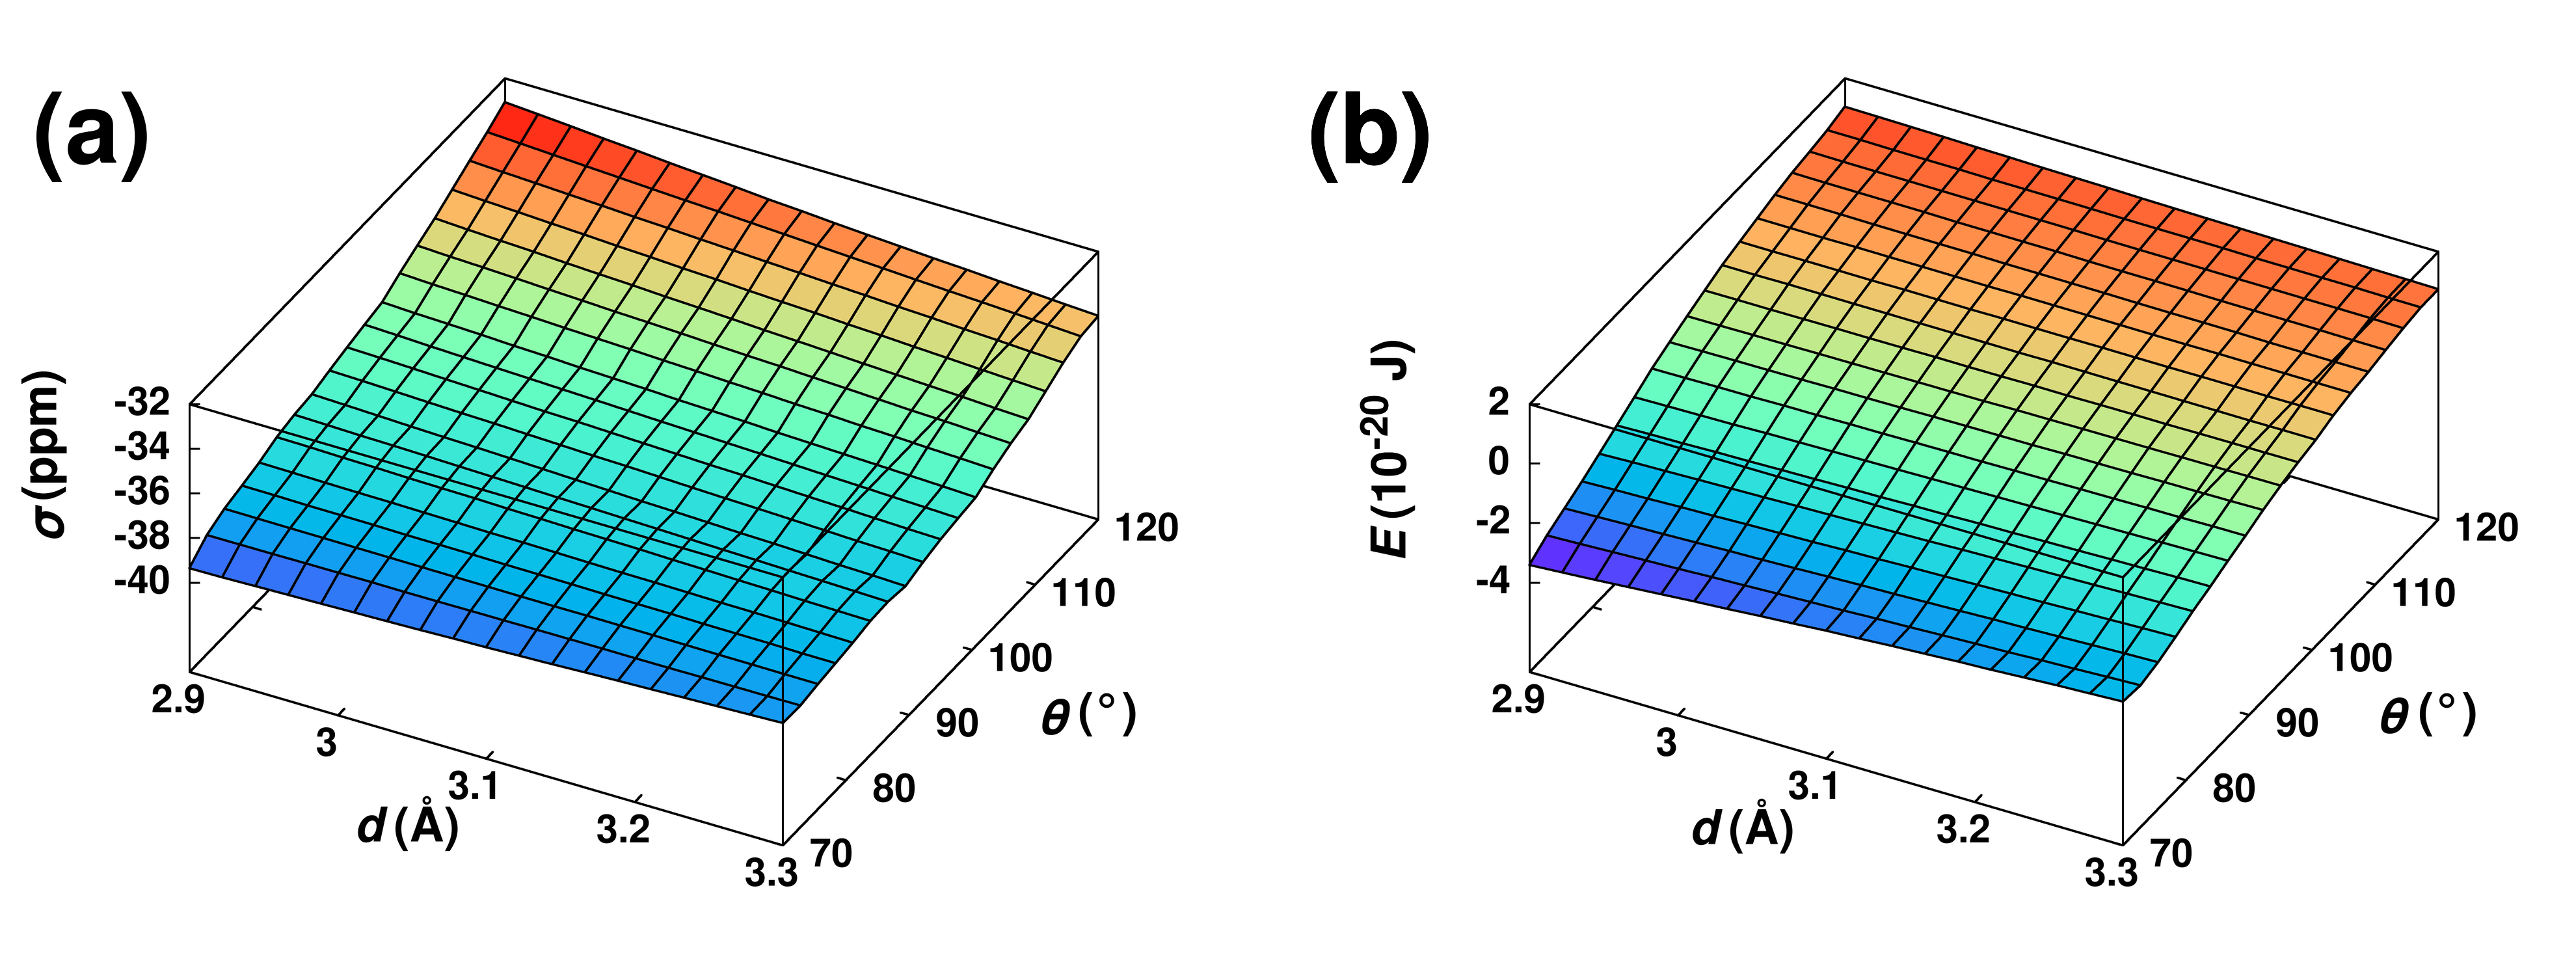
\includegraphics[width=6.5in]{figs/npistar/07.png}
\caption
      [Summary of Quantum Chemical Calculations.]{
  {\bf Summary of Quantum Chemical Calculations.}
  \\
  Plot of calculated ({\bf A}) carbonyl \cnmr{} chemical shielding ($\sigma$)
  and ({\bf B}) dipole-dipole interaction energy ($E$) as a function of the
  distance between donor oxygen and acceptor carbon ($d$) and the angle
  between carbonyl groups ($\theta$).
}
\end{figure}

\begin{doublespace}
To further examine the origin of these effects, quantum chemical calculations
were conducted on a model system, a formamide trimer in which molecules 2 and 3
form an approximately planar, head-to-tail hydrogen bonded dimer, and molecule
3 acts as a putative \npistar{} donor, with the $n_\pi$ `donor' oxygen fixed at
a distance $d$ which ranges from 2.9 \r{A} and 3.3 \r{A} from the carbonyl
carbon of molecule 2, with the O$_3\cdots$C$_2$ vector also fixed at angles
$\theta$ from 70$^\circ$ to 120$^\circ$ from the C$_2$=O$_2$ vector. To avoid
problems with the use of density functional theory to model virtual
orbitals, M\"{o}ller-Plesset second order perturbation theory (MP2) was
instead used, with a substantially larger basis set than in the previous work.
The geometry and relevant Hartree-Fock orbitals of the complex used is shown
in Figure 8.4, for $d$ = 2.9 \r{A} and $\theta = 100^\circ$. The computed
chemical shielding is shown in Figure 8.7A as a function of $d$ and $\theta$.
The shielding decreases monotonically with $\theta$, but, in contrast, the
slope of the shielding surface with respect to $d$ changes sign between
$\theta = 70^\circ$ and $\theta = 120^\circ$. This shielding surface does not
have the geometry expected if the chemical shielding dependencies on $\theta$
and $d$ were dominated by an \npipistar{} interaction, where shielding should
be maximal at $\theta$ slightly larger than 90$^\circ$ and $d$ = 2.9 \r{A},
decreasing rapidly with increasing values of $d$.
\\\\
However, the shielding surface does show a remarkable similarity to the
dipole-dipole energy between the putative donor and acceptor, as shown in
Figure 8.7B. This energy was computed using a very simple model assuming the
electric dipole vector lies along the carbonyl bond for both molecules and has
a value of 2.34 D or $7.81 \times 10^{-30}$ C$\cdot$m. As can be seen, the
dipole energy closely parallels the chemical shielding surface, monotonically
increasing with $\theta$ and inverting its slope with respect to $d$ as
$\theta$ increases. This indicates the major influence on the carbonyl \cnmr{}
chemical shielding is not an \npipistar{} interaction but rather the
electrostatic field from the neighboring carbonyl dipole. The correspondence
is not, however, exact: the chemical shielding surface shows a small negative
inflection around $\theta = 90^\circ$, which is actually slightly reversed in
the dipolar energy plot.
\end{doublespace}

\begin{figure}[h!]
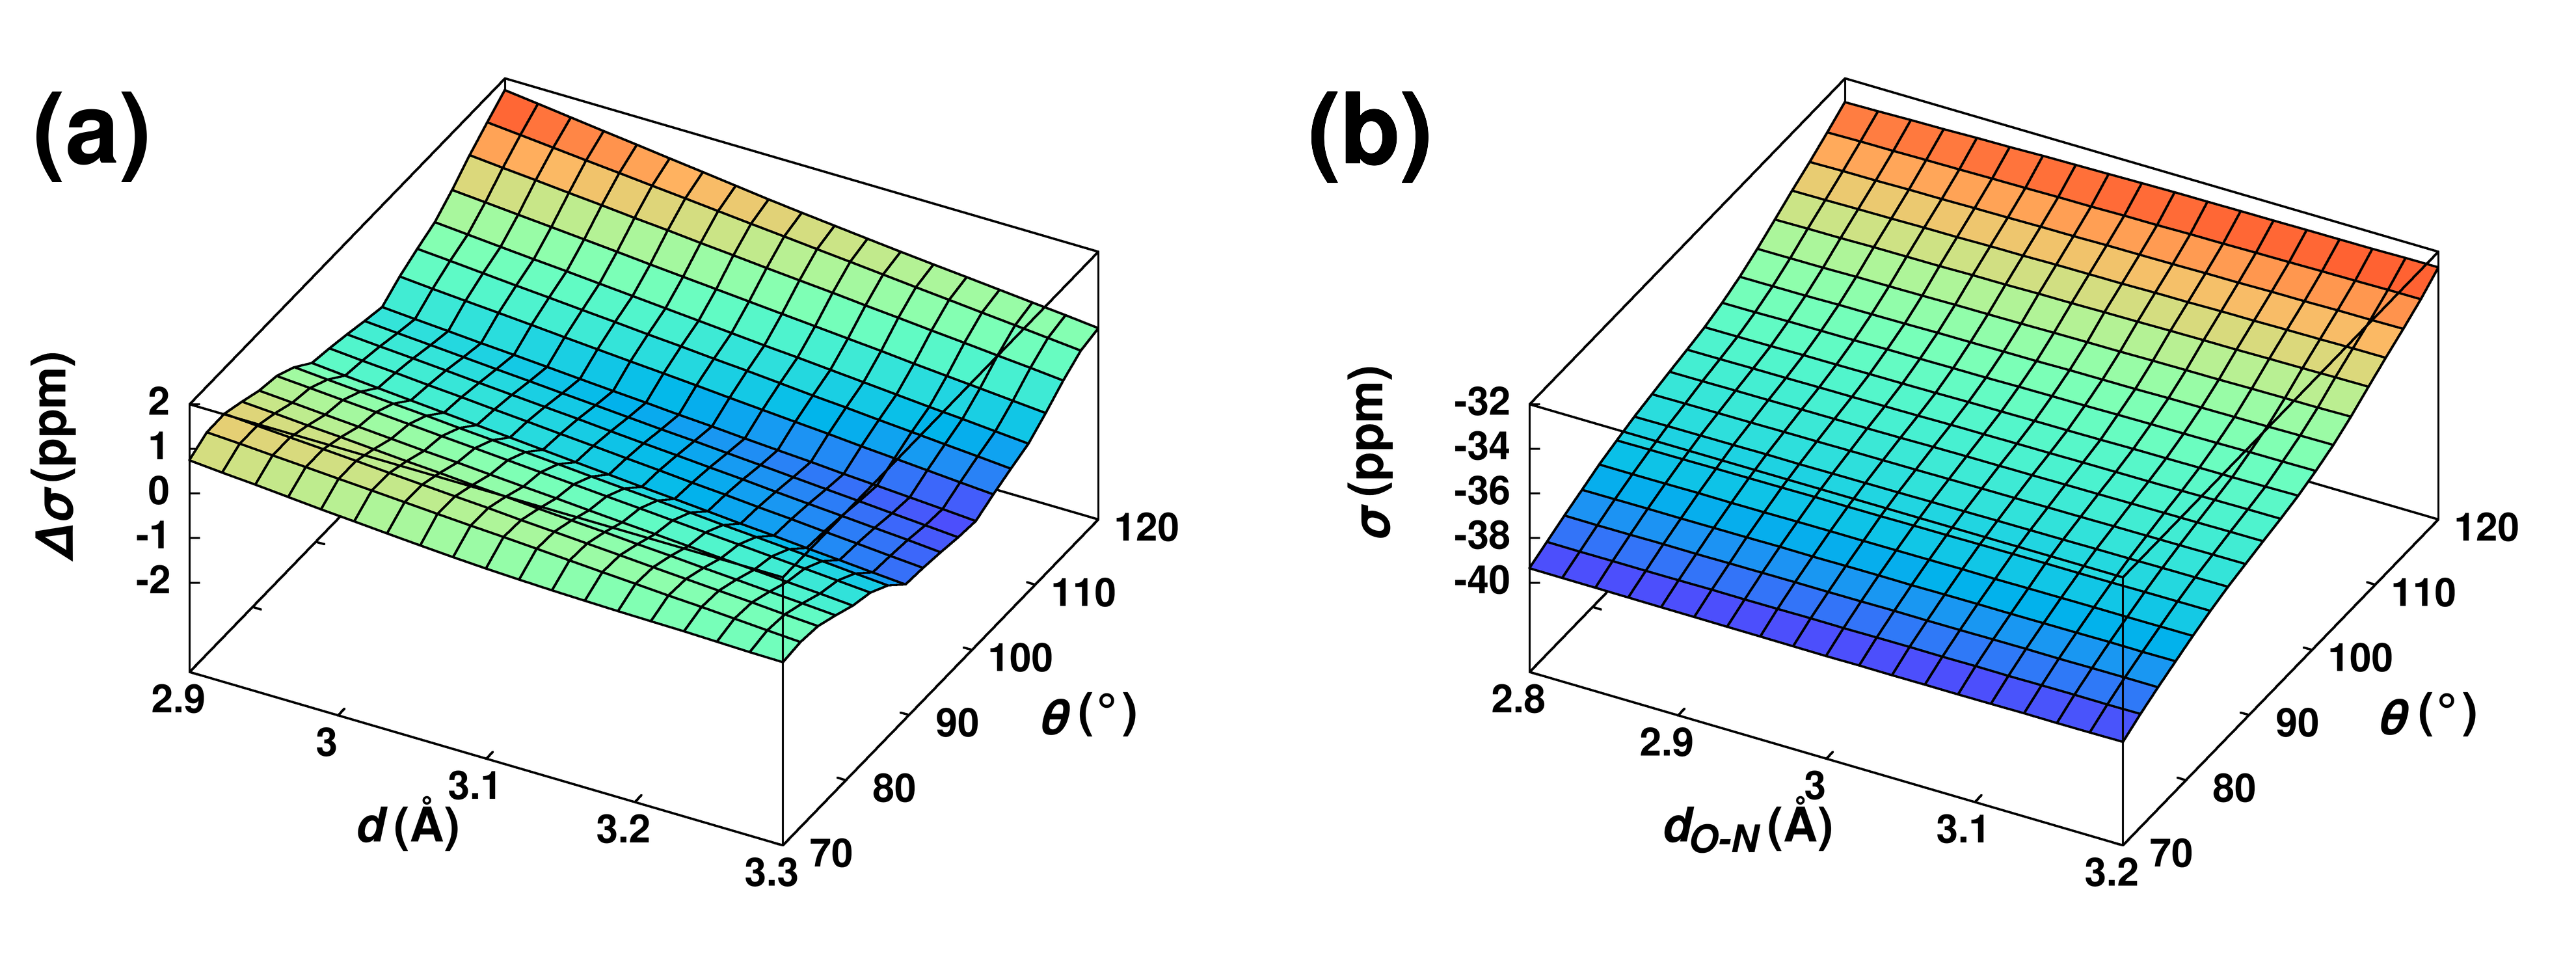
\includegraphics[width=6.5in]{figs/npistar/08.png}
\caption
      [Supplemental Quantum Chemical Results.]{
  {\bf Supplemental Quantum Chemical Results.}
  \\
  ({\bf A}) Plot of the residuals for the fit of the chemical shielding
  surface to a function proportional to the dipole-dipole energy.
  ({\bf B}) Summary of the quantum chemical calculations of the hydrogen
  bond contribution to the dipole-dipole interaction; plot of carbonyl \cnmr{}
  chemical shielding ($\sigma$) as a function of the hydrogen bond angle
  ($\theta$) and distance ($d_{O-N}$).
}
\end{figure}

\begin{doublespace}
In order to examine whether an \npipistar{} interaction might be responsible
for this inflection, the chemical shielding surface was fit to a function
proportional to the dipolar energy, under the assumption the dipole moment
vector lies along the C=O bond direction, and the best fit subtracted from the
chemical shielding surface (Figure 8.8A). The residual shows a
minimum at $\theta \sim 95^\circ$, as would be expected for an \npipistar{}
interaction, but the dip does not appear to decrease rapidly as $d$ increases,
as an orbital overlap term would. In fact, the residual is slightly larger at
$d$ = 3.3 \r{A} than at 2.9 \r{A} (1.3 ppm vs. 1.1 ppm).
\\\\
From the fit of the shielding surface to the estimated dipole interaction
energy, with the assumption the magnitude of the electric dipole moment is
that of a formamide monomer (3.7 D), a dependence of chemical shielding on
field of $-190$ ppm/a.u. was obtained (1 atomic unit (a.u.) of electric field
equals $5.142\times10^{11}$ V/m). Direct calculations of the dependence of the
shielding of an isolated formamide on an external applied field along the C=O
bond direction gave a value of $-150$ ppm/a.u. However, it is highly likely
that this estimation of the dipole-dipole interaction for two amides is low.
Firstly, higher electric multipole terms were neglected in the calculation,
and these are likely to be substantial for a moiety as asymmetric as a peptide
linkage, at these close proximities. Second, the interaction of the dipoles
is likely to be enhanced by the highly polarizable hydrogen bond, which is
necessarily omitted in the monomer model. Agreement of the model with direct
estimates of the effect of electric field on shielding is therefore rather
good.
\\\\
The dependence of chemical shielding on hydrogen bonding strength for all
combinations of $d$ and $\theta$ was examined as a function of the hydrogen
bond distance $d_{O-N}$ (see Supplemental Figure 8.8B). In accordance with the
results of Wishart and others
\cite{cisnetti:cpc2004,neal:jbnmr2003,markwick:jacs2004}, and contrary
to initial na\"{i}ve expectations, the effect was very small and independent of
the position of the putative \npipistar{} donor carbonyl.
\end{doublespace}

\begin{figure}[h!]
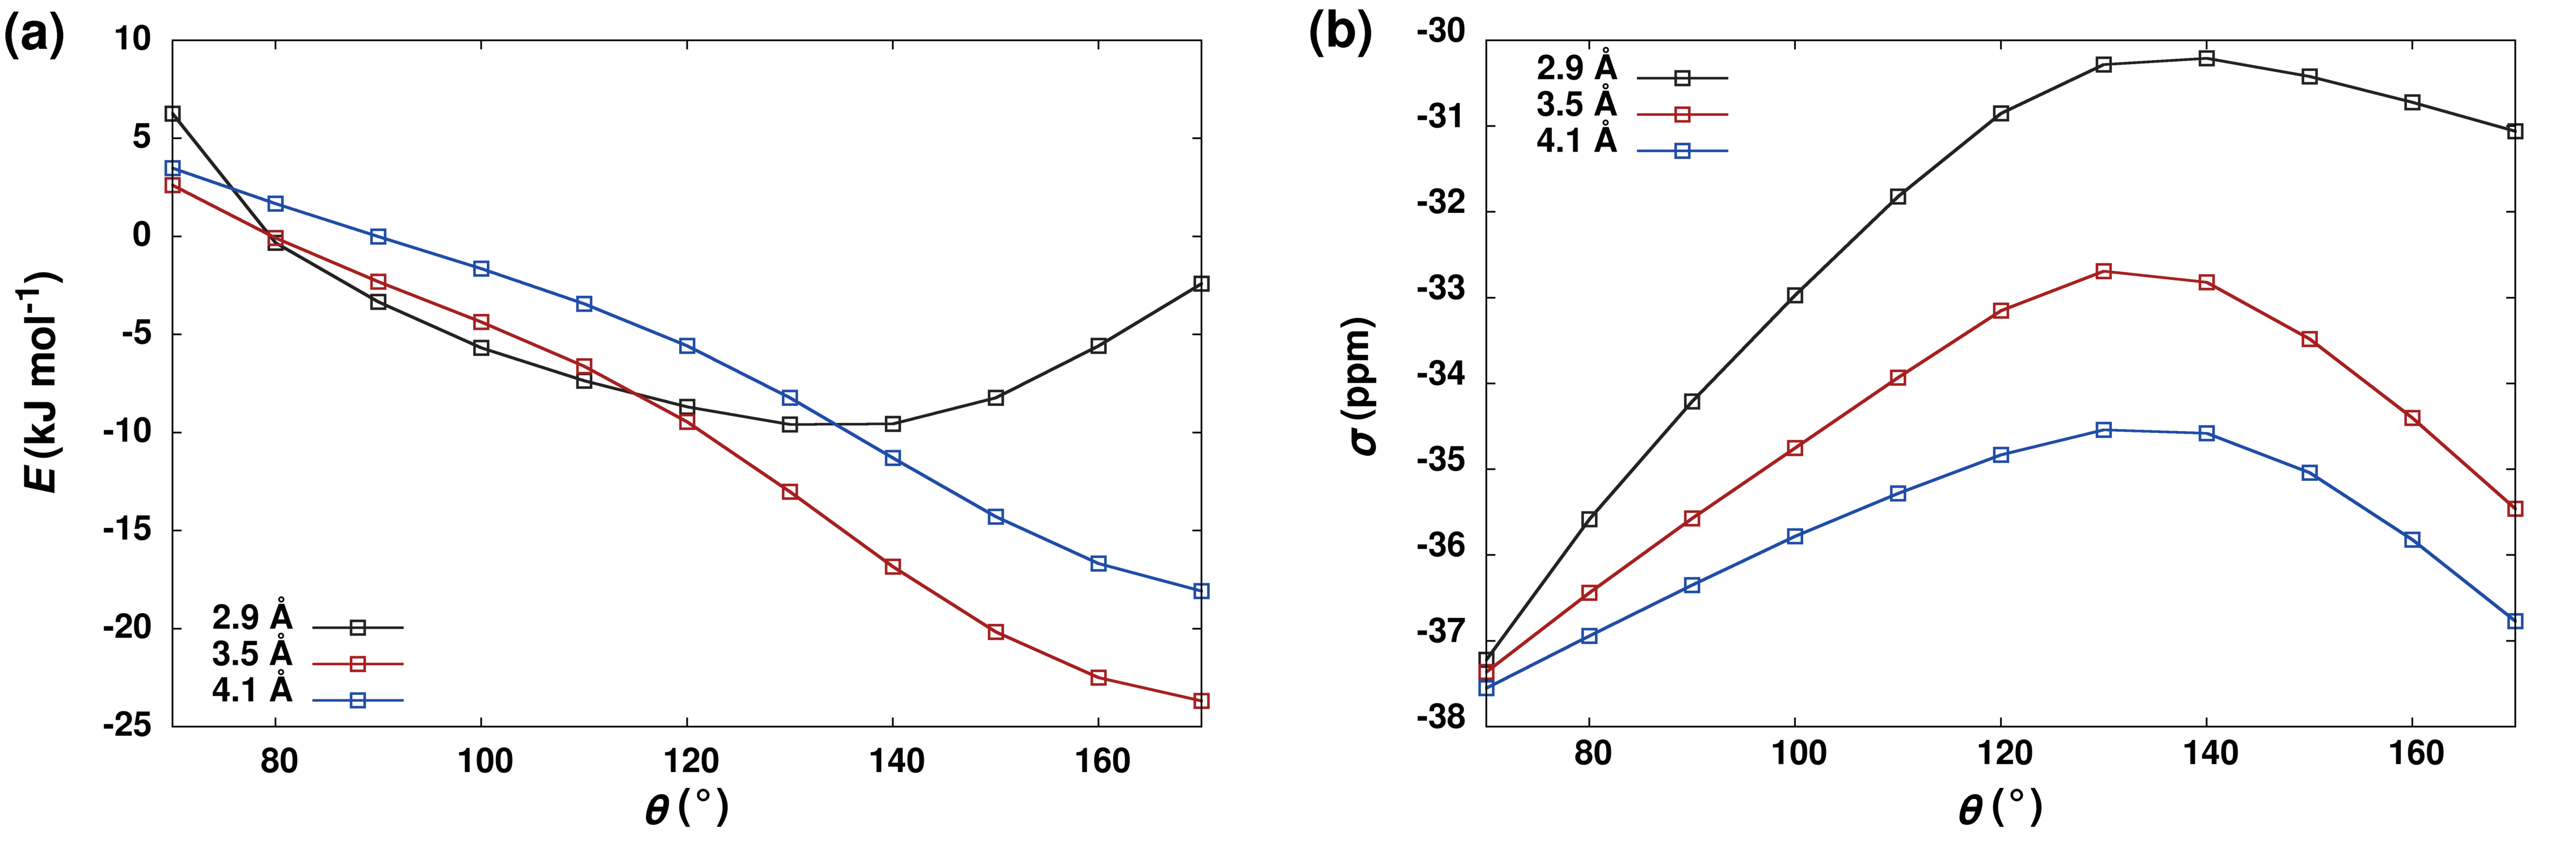
\includegraphics[width=6.5in]{figs/npistar/09.png}
\caption
   [Summary of Quantum Chemical Calculations for `End-On' Dipole Interaction.]
  {{\bf
    Summary of Quantum Chemical Calculations for `End-On' Dipole Interaction.
  }
  \\
  Plots of ({\bf A}) interaction energy and ({\bf B}) carbonyl \cnmr{} chemical
  shielding ($\sigma$) as a function of the angle between the carbonyls
  ($\theta$) for three different distances ($d$) between the donor oxygen
  and acceptor carbon.
}
\end{figure}

\begin{doublespace}
For the sake of completeness, the effect of an `end-on' carbonyl-carbonyl
interaction was examined, using a dimeric cluster in which the `donor' carbonyl
bond was parallel to the `donor' oxygen-`acceptor' carbon vector, resulting in
a possible \nspistar{} interaction. As can be seen in Figure 8.9, for values of
$d$ ranging from 2.9 \r{A} to 4.1 \r{A}, the chemical shielding also follows
the negative of the dipolar interaction energy over the range
$70^\circ < \theta < 120^\circ$, with little evidence of any effect of orbital
overlap on chemical shielding.
\\\\
One other outcome of the calculations is of possible note. While there was
little discernible effect of the proposed \nspistar{} or \npipistar{}
interactions on the shielding of the carbonyl carbon or the length of the
carbonyl bond, substantial pyramidalization of the amide nitrogen was observed
at low values of $d$ and values of $\theta$ close to 90$^\circ$. This would
indicate that the primary effect of the `donor' carbonyl might not be on the
carbonyl $\pi$ bond \emph{per se}, but on its delocalization over the entire
amide group. There was also a substantial lengthening of the carbon-nitrogen
bond -- consistent with a reduced bond order -- accompanied by substantial
changes in the computed \nnmr{} chemical shielding. Thus, while no evidence
was found of effects from \nspistar{} interactions on the \cnmr{} NMR
spectroscopy or the energetics of the system, such interactions might be
detectable in \nnmr{} chemical shifts. Unfortunately, \nnmr{} shifts are known
to be much more dispersed than carbonyl \cnmr{} shifts and are susceptible to
a wide range of influences, so disentangling the interaction in real proteins
might be a Herculean task.
\end{doublespace}

\section{Discussion and Conclusions}

\begin{doublespace}
When the molecular orbitals for the trimeric complex are examined in detail, 
the above results become clear. It is in fact misleading to think of amide 
groups as being dominated by the carbonyl $\pi$ bond. The highest occupied
molecular orbital (HOMO) of the formamide trimer in fact consists almost
entirely of $p_z$ orbitals on the N and O, with wavefunctions of opposite sign.
This is depicted in Figure 8.4A for the Hartree-Fock HOMO of the hydrogen bond
donor (energy = $-0.377$ Ha). The orbital is slightly bonding with respect to
the carbonyl, but the carbonyl carbon overall has very little contribution to
the molecular orbital. The equivalent orbital of the putative acceptor
(Figure 8.4B) has somewhat lower energy ($-0.438$ Ha) but shows remarkably
little mixing with other molecular orbitals, and in particular little mixing
with the $n_\pi$ orbital of the putative \npipistar{} donor (Figure 8.4C). That
orbital has in fact a very similar energy ($-0.465$ Ha), and at other
geometries -- specifically lower values of $\theta$, mixes with the HOMO of
the acceptor. The reason for this is quite simple: because the HOMO has only a
very small contribution for carbonyl carbon orbitals, bringing the $n_\pi$
orbital closer to it has very little effect. The mixing that is present at
smaller values of $\theta$ in fact seems to be partly responsible for the
increased pyramidalization of the nitrogen of the acceptor at those
orientations. We see no evidence of any orbital mixing that could be attributed
to \npipistar{} interactions. Given the weakness of the mixing with orbitals
that are very close in energy to $n_\pi$ it is implausible that substantial
mixing would be observed with an orbital almost a Hartree higher in energy.
\\\\
In conclusion, quantum chemical calculations, experimental carbonyl \cnmr{}
chemical shifts and structural data indicate that a simple electrostatic
dipole-dipole interaction explains the large downfield carbonyl \cnmr{}
chemical shift in an $\alpha$-helix. There is no evidence for a significant
contribution from an \npistar{} interaction to the carbonyl bond. The single
indication of \npistar{} interactions seems to be a substantial lengthening of
the carbon-nitrogen bond and pyramidalization of the nitrogen at $\theta$
angles favorable for these interactions. In fact, such pyramidalization seems
to be a logical consequence of the electronic structure of amides, whose $\pi$
orbitals are delocalized over the whole system.
\end{doublespace}

\bibliographystyle{abbrv}
\bibliography{bworley}



\chapter{Summary and Future Directions}

FIXME \cite{worley:abio2013}.

\bibliographystyle{abbrv}
\bibliography{bworley}



% ============================================================================

\appendix

\listoffigures
\addcontentsline{toc}{chapter}{List of Figures}

\listoftables
\addcontentsline{toc}{chapter}{List of Tables}

\end{document}
